% ============================================================
%  Anexo III - Análisis y Diseño del Sistema
%  DocumentChain - Sistema de Gestión Documental con Blockchain
% ============================================================
\documentclass[11pt, a4paper]{article}

\usepackage{fontspec}
\usepackage[spanish]{babel}
\usepackage{graphicx}
\usepackage{float}
\usepackage{amsmath}
\usepackage{xcolor}
\usepackage[protrusion=true,expansion=false]{microtype}
\usepackage{longtable}
\usepackage{array}
\usepackage{booktabs}
\usepackage{multirow}
\usepackage{caption}
\usepackage{pdflscape}
\usepackage{eso-pic}
\usepackage{tikz}
\usetikzlibrary{calc}
\usepackage[
    colorlinks = true,
    linkcolor  = black,
    urlcolor   = black,
    citecolor  = black
]{hyperref}

\usepackage{geometry}
\geometry{
    left       = 2.5cm,
    right      = 2.5cm,
    top        = 3cm,
    bottom     = 2.5cm,
    headheight = 55pt,
    headsep    = 0.8cm
}

\usepackage{fancyhdr}
\pagestyle{fancy}
\fancyhf{}

\lhead{
\includegraphics[height=1.25cm]{USAL-Logo-3820702873.png}}
\rhead{\shortstack[r]{\fontsize{10}{12}\selectfont\textbf{\tituloInforme}\\[-1pt]\fontsize{10}{12}\selectfont\subtituloInforme}}

\renewcommand{\headrulewidth}{0pt}
\renewcommand{\footrulewidth}{0pt}

\cfoot{%
        \color{gray}\rule[0.5ex]{0.4\textwidth}{0.8pt}%
        \hspace{0.5cm}%
        \textcolor{black}{\textbf{\thepage}}%
        \hspace{0.5cm}%
        \color{gray}\rule[0.5ex]{0.4\textwidth}{0.8pt}%
}

% ============================================================
% SOPORTE ENCABEZADO/PIE EN PÁGINAS APAISADAS (landscape)
% ============================================================
\newif\iflscape\lscapefalse

\let\origlandscape\landscape
\let\origendlandscape\endlandscape
\renewenvironment{landscape}{%
    \origlandscape\lscapetrue\thispagestyle{empty}%
}{%
    \origendlandscape\lscapefalse%
}

\AddToShipoutPictureFG{%
    \iflscape
        \begin{tikzpicture}[remember picture, overlay]
            \node[rotate=90, anchor=center, inner sep=0pt]
                at ([xshift=1.0cm]current page.west)
                {\makebox[\textheight]{%
                    
\includegraphics[height=1.1cm]{USAL-Logo-3820702873.png}\hfill%
                    \shortstack[r]{\fontsize{10}{12}\selectfont\textbf{\tituloInforme}\\[-1pt]\fontsize{10}{12}\selectfont\subtituloInforme}}};
            \node[rotate=90, anchor=center, inner sep=0pt]
                at ([xshift=-1.5cm]current page.east)
                {\color{gray}\rule[0.5ex]{5cm}{0.8pt}%
                 \hspace{0.4cm}\textcolor{black}{\textbf{\thepage}}\hspace{0.4cm}%
                 \color{gray}\rule[0.5ex]{5cm}{0.8pt}};
        \end{tikzpicture}%
    \fi%
}

\newcommand{\tituloInforme}{Anexo III: Análisis y diseño del sistema}
\newcommand{\subtituloInforme}{Sistema de Gestión Documental mediante Blockchain}
\newcommand{\asignatura}{Trabajo de Fin de Grado}
\newcommand{\autorUno}{David Pérez Velasco}
\newcommand{\tutorUno}{Gabriel Villarrubia González}
\newcommand{\tutorDos}{Sergio García González}

\begin{document}

\begin{titlepage}
    \centering
    \vspace*{1.5cm}
    {\scshape\LARGE Universidad de Salamanca \par}
    \vspace{1cm}
    {\scshape\Large Grado en Ingeniería Informática \par}
    \vspace{1.5cm}
    {\huge\bfseries ANEXO III \par}
    \vspace{0.5cm}
    {\Large\bfseries Análisis y Diseño del Sistema \par}
    \vspace{0.3cm}
    {\large\itshape Sistema de Gestión Documental mediante Blockchain \par}
    \vspace{1.8cm}
    
\includegraphics[width=0.28\textwidth]{USAL-Logo-3820702873.png}

    \vspace{2.2cm}

    {\Large\itshape \autorUno \par}
    \vspace{1.5cm}
    {\large Tutores: \par}
    \vspace{0.3cm}
    {\large \tutorUno \par}
    \vspace{0.2cm}
    {\large \tutorDos \par}

    \vspace{2cm}
    {\large Julio 2026}
    \vspace{0.5cm}

    \asignatura
    \vspace{1cm}
\end{titlepage}

\setcounter{page}{2}
\pagestyle{fancy}

\tableofcontents
\newpage

\listoffigures
\newpage

\listoftables
\newpage

% ============================================================
% PARTE A — MODELO DE ANÁLISIS
% ============================================================
\section{Introducción}

En este anexo se documenta la transición desde los requisitos del sistema (Anexo I) hasta la arquitectura final de la solución. El documento se organiza en dos grandes bloques, en coherencia con la normativa CCII-N2016-02. La Parte A recoge el modelo de análisis: modelo del dominio, clases de análisis según el patrón Boundary-Control-Entity (BCE) y los diagramas de secuencia de análisis correspondientes a los 43 casos de uso del catálogo funcional. La Parte B aborda el diseño arquitectónico y procedimental: arquitectura de capas, patrones de diseño, subsistemas, clases de diseño, diagramas de secuencia de realización técnica, diseño de la base de datos y modelo de despliegue.

\section{Modelo de dominio}

El modelo de dominio representa las entidades del negocio, sus atributos y las relaciones entre ellas, abstrayendo los detalles de implementación. La Figura~\ref{fig:class-analysis} muestra el diagrama de clases de análisis del sistema DocumentChain.

\begin{figure}[H]
    \centering
    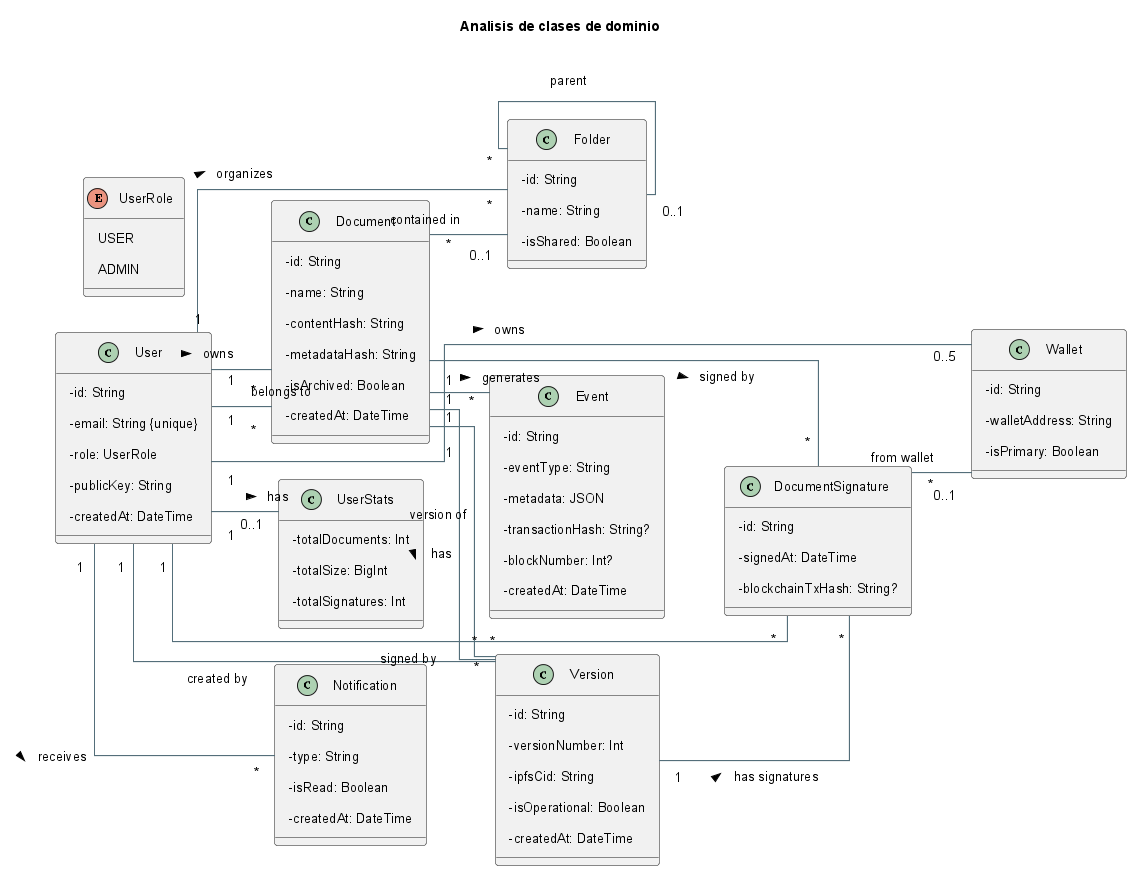
\includegraphics[width=0.9\textwidth]{diagramas/class-analysis.png}
    \caption{Modelo de dominio — Diagrama de clases de análisis}
    \label{fig:class-analysis}
\end{figure}

\section{Clases de análisis BCE}

El patrón Boundary-Control-Entity organiza las clases del sistema en tres categorías: clases de frontera (\textit{Boundary}), que gestionan la interacción con los actores; clases de control (\textit{Control}), que implementan la lógica de negocio; y clases de entidad (\textit{Entity}), que representan los objetos persistentes del dominio. La Figura~\ref{fig:class-analysis-bce} presenta esta clasificación para los siete paquetes funcionales del sistema, y la Tabla~\ref{tab:bce-clasificacion} detalla la asignación de cada clase a su paquete.

\begin{figure}[H]
    \centering
    
\includegraphics[width=0.95\linewidth]{diagramas/class-analysis-bce.png}
    \caption{Clases de análisis BCE}
    \label{fig:class-analysis-bce}
\end{figure}

\begin{table}[H]
\centering
\small
\renewcommand{\arraystretch}{1.3}
\begin{tabular}{|l|l|l|l|}
\hline
\textbf{Paquete funcional} & \textbf{Boundary} & \textbf{Control} & \textbf{Entity} \\
\hline
Acceso y cuenta & Interfaz Registro, Interfaz Login, Interfaz Perfil & Controlador Autenticación, Controlador Usuario & Usuario, Sesión \\
\hline
Wallets & Interfaz Wallet & Controlador Wallet & Wallet \\
\hline
Gestión documental & Interfaz Biblioteca, Interfaz Detalle Documento & Controlador Documento & Documento, Carpeta \\
\hline
Versionado & Interfaz Versiones & Controlador Versión & Versión \\
\hline
Firmas & Interfaz Firma & Controlador Firma & Firma \\
\hline
Compartición & Interfaz Compartición & Controlador Compartición & Permiso \\
\hline
Auditoría y administración & Interfaz Auditoría, Interfaz Administración & Controlador Auditoría, Controlador Administración & EventoAuditoría, Notificación, Estadística, RolSistema \\
\hline
\end{tabular}
\caption{Clasificación BCE por paquete funcional}
\label{tab:bce-clasificacion}
\end{table}


\section{Diagramas de secuencia de análisis (BCE)}

Los diagramas de secuencia de análisis modelan la interacción entre actores y objetos del dominio utilizando el patrón BCE. Cada diagrama representa un caso de uso del catálogo funcional (Anexo I) y emplea el estilo definido en \texttt{\_sequence-bce-style.puml}: actores del catálogo canónico (Usuario no logueado, Usuario logueado, Administrador), nombres en español funcional y ausencia de detalles de infraestructura técnica. Las figuras se presentan agrupadas por paquete funcional.

\subsection{Paquete: Acceso y cuenta (UC-0001 a UC-0014)}

\begin{figure}[H]\centering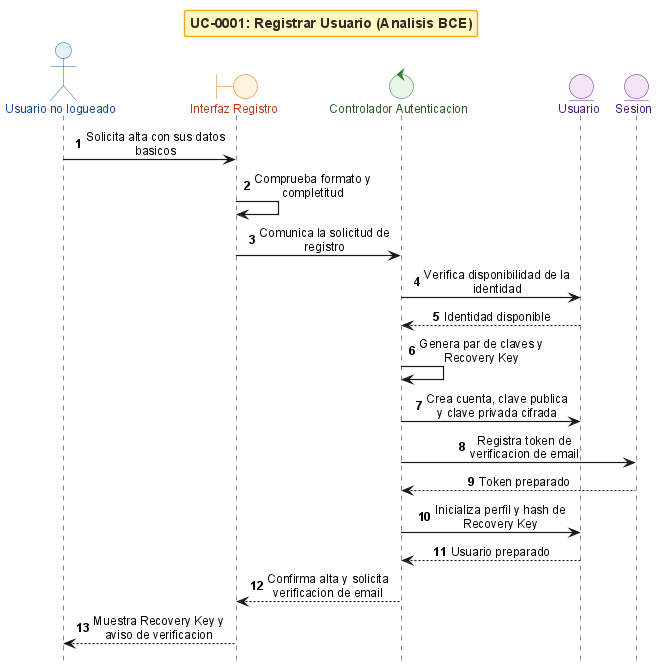
\includegraphics[width=0.92\textwidth]{diagramas/seq-bce-uc0001-register.png}\caption{Análisis BCE — UC-0001: Registrar Usuario}\label{fig:seq-bce-uc0001}\end{figure}
\begin{figure}[H]\centering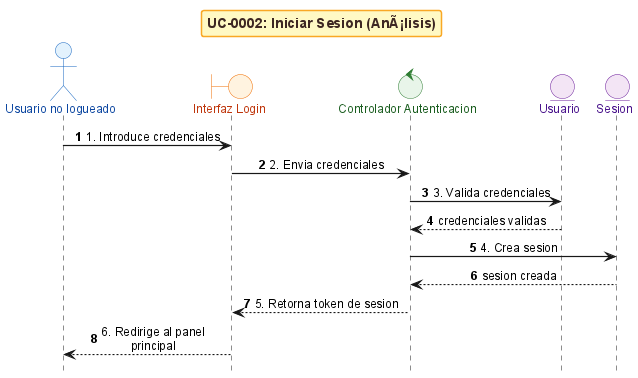
\includegraphics[width=0.92\textwidth]{diagramas/seq-bce-uc0002-login.png}\caption{Análisis BCE — UC-0002: Iniciar Sesión}\label{fig:seq-bce-uc0002}\end{figure}
\begin{figure}[H]\centering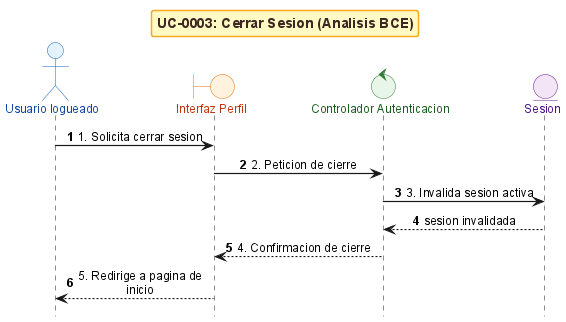
\includegraphics[width=0.85\textwidth]{diagramas/seq-bce-uc0003-logout.png}\caption{Análisis BCE — UC-0003: Cerrar Sesión}\label{fig:seq-bce-uc0003}\end{figure}
\begin{figure}[H]\centering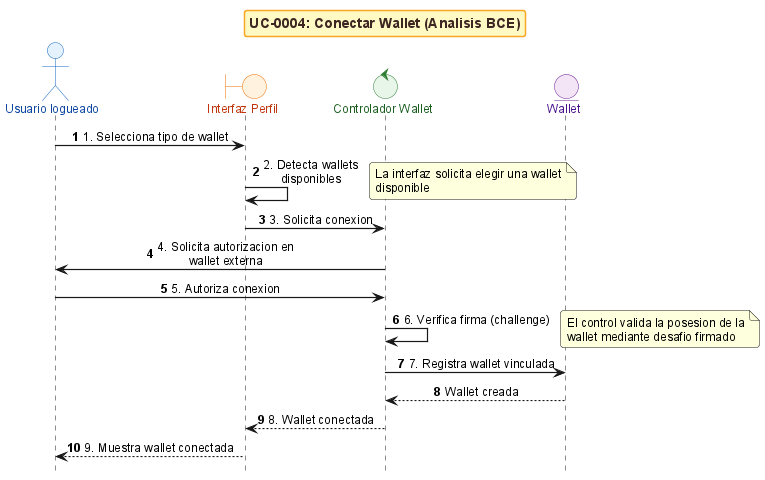
\includegraphics[width=0.92\textwidth]{diagramas/seq-bce-uc0004-wallet.png}\caption{Análisis BCE — UC-0004: Conectar Wallet}\label{fig:seq-bce-uc0004}\end{figure}
\begin{figure}[H]\centering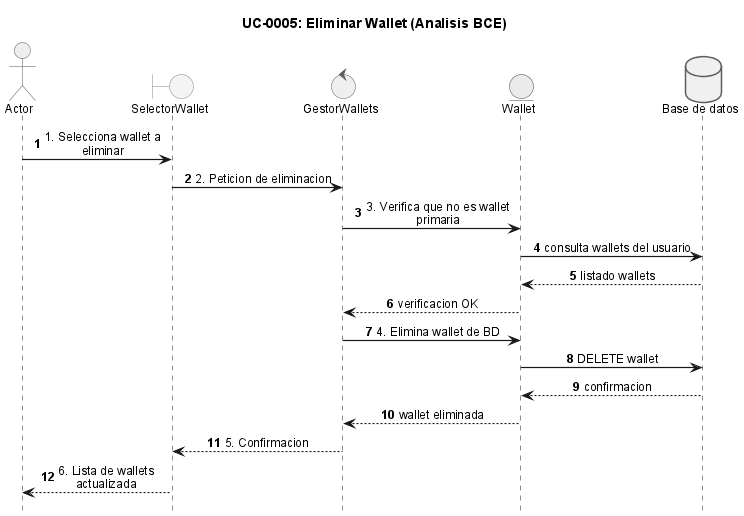
\includegraphics[width=0.85\textwidth]{diagramas/seq-bce-uc0005-delete-wallet.png}\caption{Análisis BCE — UC-0005: Eliminar Wallet}\label{fig:seq-bce-uc0005}\end{figure}
\begin{figure}[H]\centering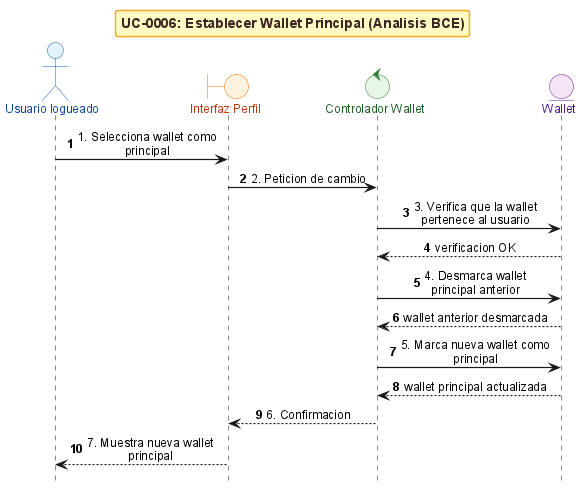
\includegraphics[width=0.88\textwidth]{diagramas/seq-bce-uc0006-primary-wallet.png}\caption{Análisis BCE — UC-0006: Establecer Wallet Principal}\label{fig:seq-bce-uc0006}\end{figure}
\begin{figure}[H]\centering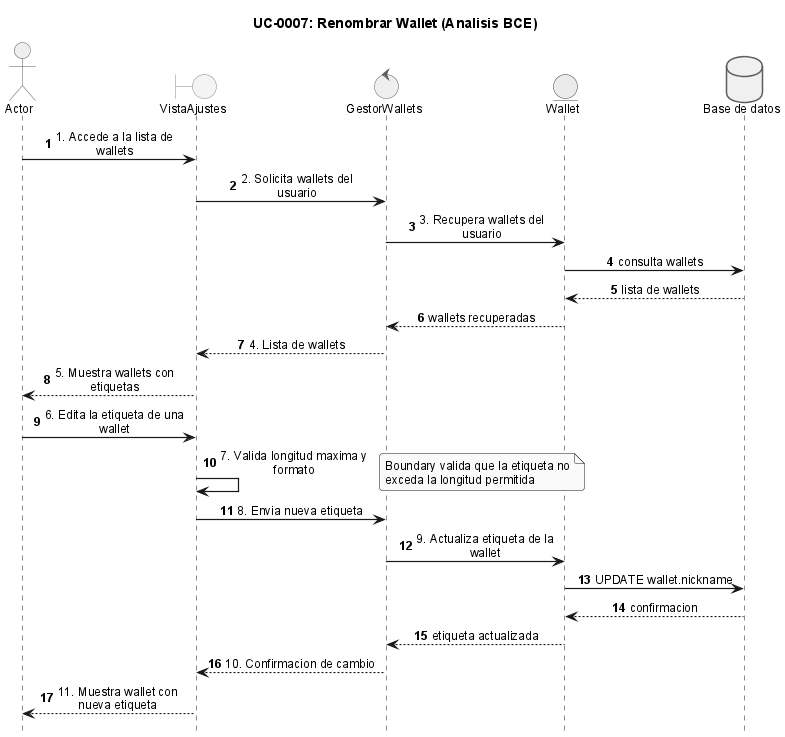
\includegraphics[width=0.92\textwidth]{diagramas/seq-bce-uc0007-rename-wallet.png}\caption{Análisis BCE — UC-0007: Renombrar Wallet}\label{fig:seq-bce-uc0007}\end{figure}
\begin{figure}[H]\centering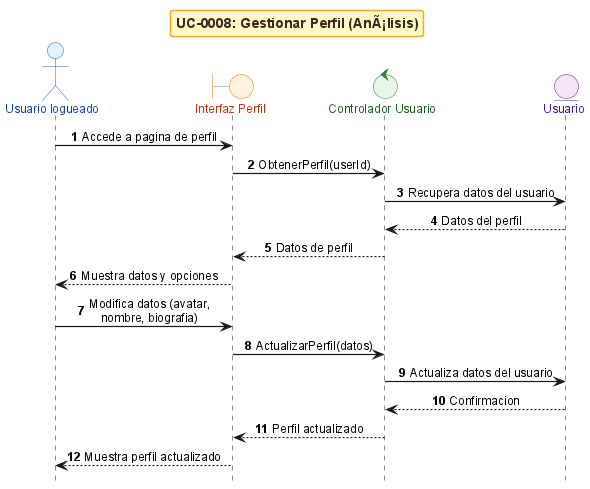
\includegraphics[width=0.92\textwidth]{diagramas/seq-bce-uc0008-profile.png}\caption{Análisis BCE — UC-0008: Gestionar Perfil}\label{fig:seq-bce-uc0008}\end{figure}
\begin{figure}[H]\centering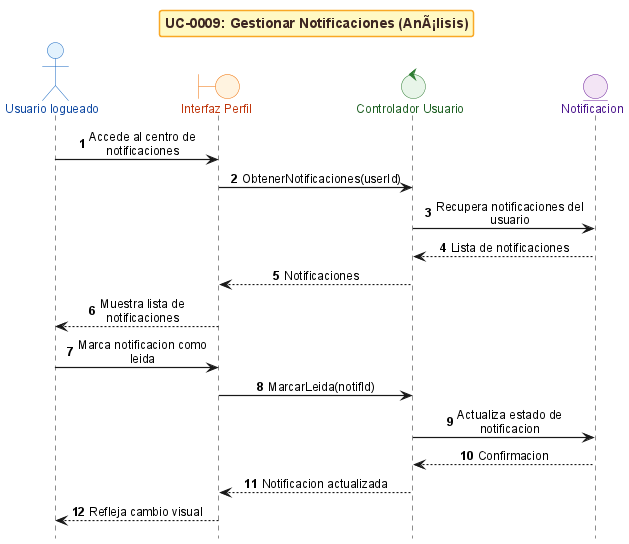
\includegraphics[width=0.92\textwidth]{diagramas/seq-bce-uc0009-notifications.png}\caption{Análisis BCE — UC-0009: Consultar Notificaciones}\label{fig:seq-bce-uc0009}\end{figure}
\begin{figure}[H]\centering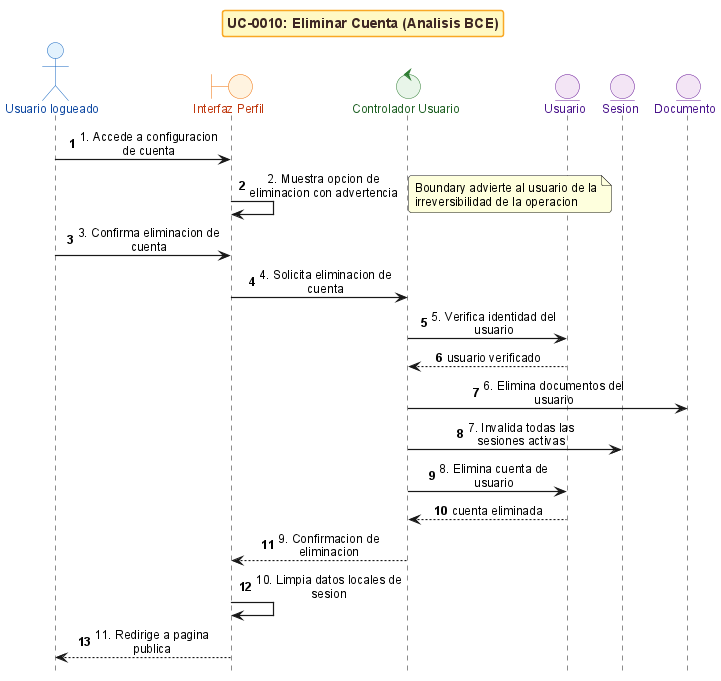
\includegraphics[width=0.92\textwidth]{diagramas/seq-bce-uc0010-delete-account.png}\caption{Análisis BCE — UC-0010: Eliminar Cuenta}\label{fig:seq-bce-uc0010}\end{figure}
\begin{figure}[H]\centering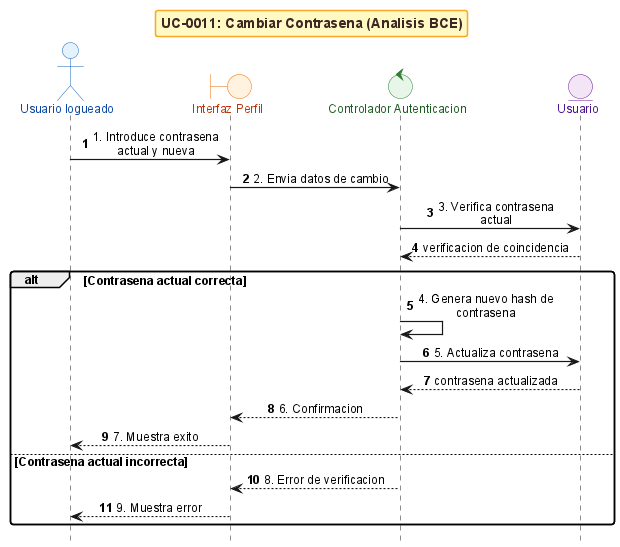
\includegraphics[width=0.88\textwidth]{diagramas/seq-bce-uc0011-change-password.png}\caption{Análisis BCE — UC-0011: Cambiar Contraseña}\label{fig:seq-bce-uc0011}\end{figure}
\begin{figure}[H]\centering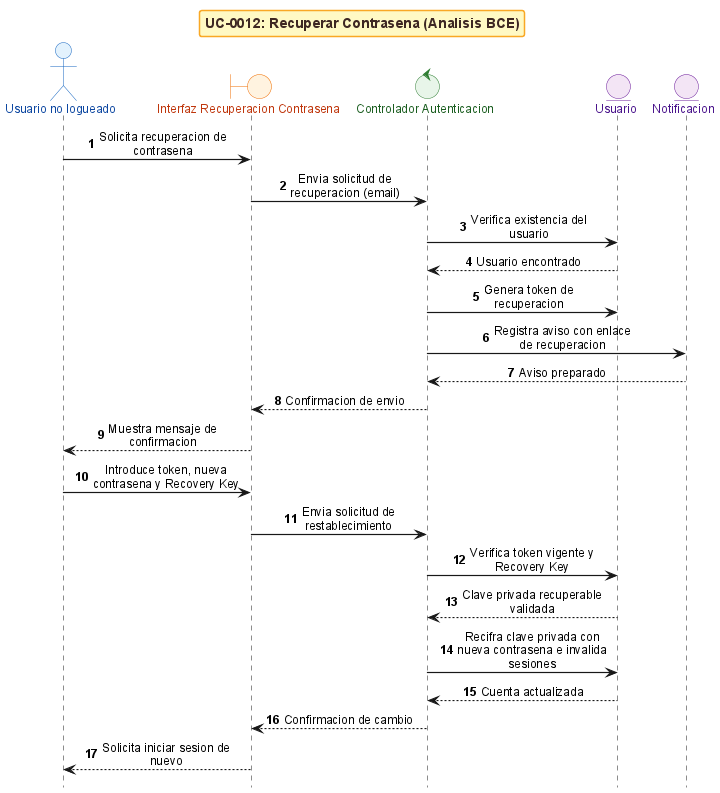
\includegraphics[width=0.90\textwidth]{diagramas/seq-bce-uc0012-recover-password.png}\caption{Análisis BCE — UC-0012: Recuperar Contraseña}\label{fig:seq-bce-uc0012}\end{figure}
\begin{figure}[H]\centering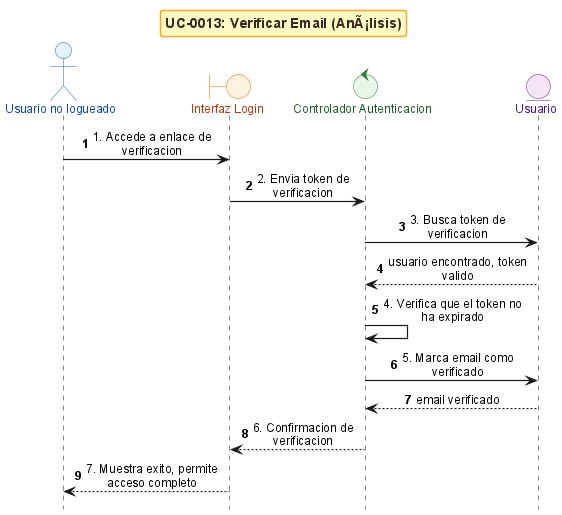
\includegraphics[width=0.88\textwidth]{diagramas/seq-bce-uc0013-verify-email.png}\caption{Análisis BCE — UC-0013: Verificar Email}\label{fig:seq-bce-uc0013}\end{figure}
\begin{figure}[H]\centering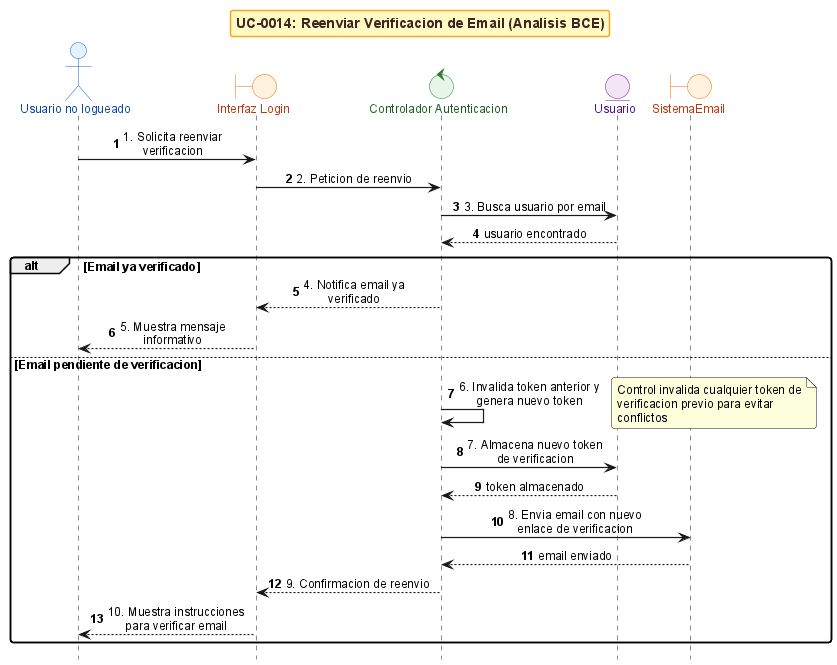
\includegraphics[width=0.92\textwidth]{diagramas/seq-bce-uc0014-resend-verification.png}\caption{Análisis BCE — UC-0014: Reenviar Verificación}\label{fig:seq-bce-uc0014}\end{figure}

\subsection{Paquete: Gestión de documentos (UC-0015 a UC-0025)}

\begin{figure}[H]\centering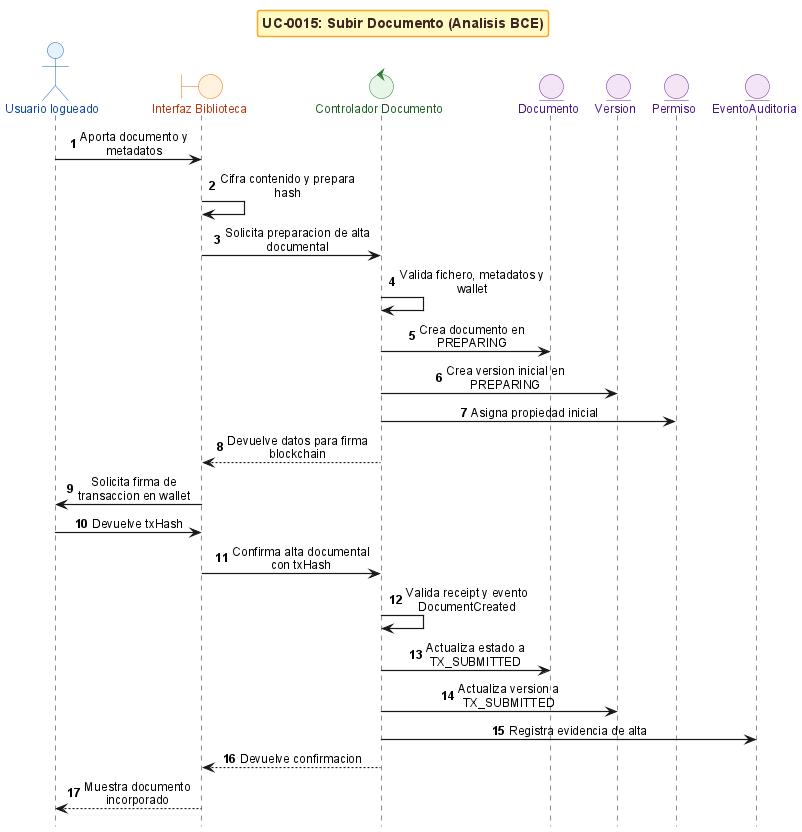
\includegraphics[width=0.92\textwidth]{diagramas/seq-bce-uc0015-upload.png}\caption{Análisis BCE — UC-0015: Subir Documento}\label{fig:seq-bce-uc0015}\end{figure}
\begin{figure}[H]\centering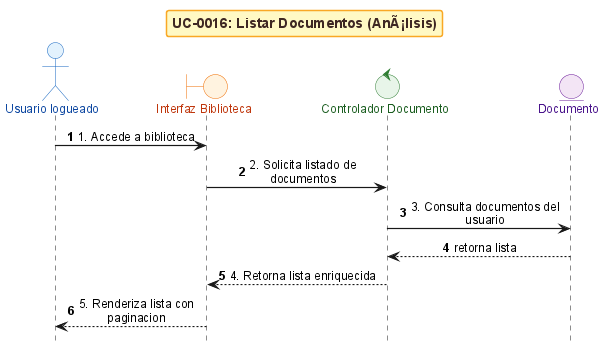
\includegraphics[width=0.92\textwidth]{diagramas/seq-bce-uc0016-list.png}\caption{Análisis BCE — UC-0016: Listar Documentos}\label{fig:seq-bce-uc0016}\end{figure}
\begin{figure}[H]\centering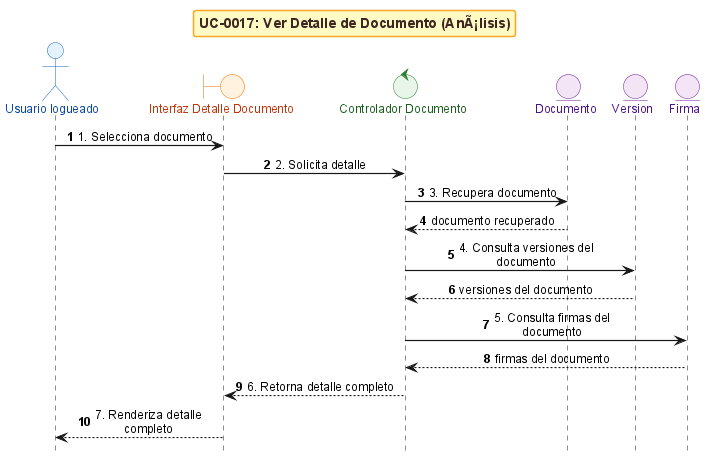
\includegraphics[width=0.92\textwidth]{diagramas/seq-bce-uc0017-detail.png}\caption{Análisis BCE — UC-0017: Ver Detalle}\label{fig:seq-bce-uc0017}\end{figure}
\begin{figure}[H]\centering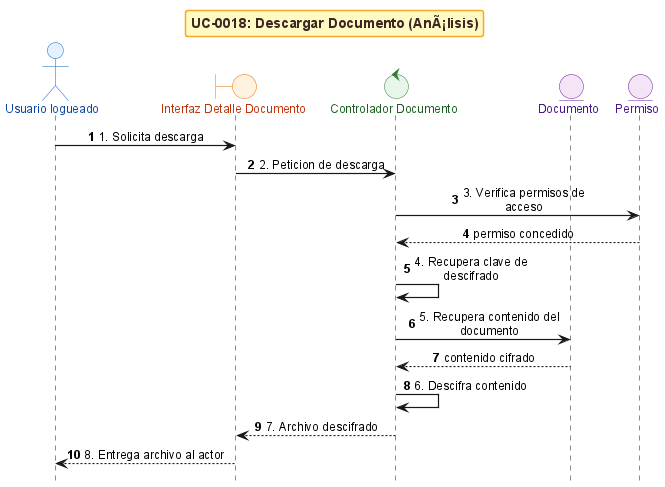
\includegraphics[width=0.92\textwidth]{diagramas/seq-bce-uc0018-download.png}\caption{Análisis BCE — UC-0018: Descargar Documento}\label{fig:seq-bce-uc0018}\end{figure}
\begin{figure}[H]\centering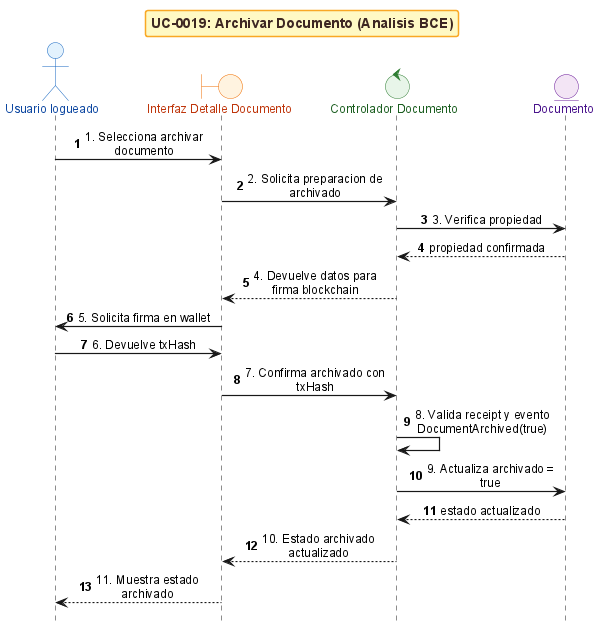
\includegraphics[width=0.92\textwidth]{diagramas/seq-bce-uc0019-archive.png}\caption{Análisis BCE — UC-0019: Archivar Documento}\label{fig:seq-bce-uc0019}\end{figure}
\begin{figure}[H]\centering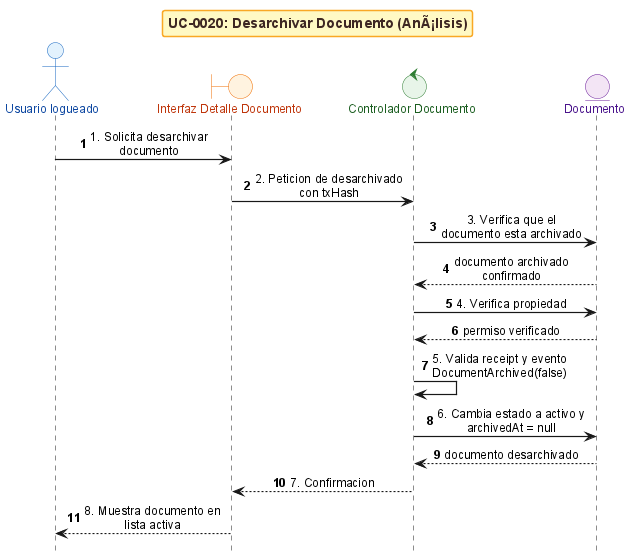
\includegraphics[width=0.90\textwidth]{diagramas/seq-bce-uc0020-unarchive.png}\caption{Análisis BCE — UC-0020: Desarchivar Documento}\label{fig:seq-bce-uc0020}\end{figure}
\begin{figure}[H]\centering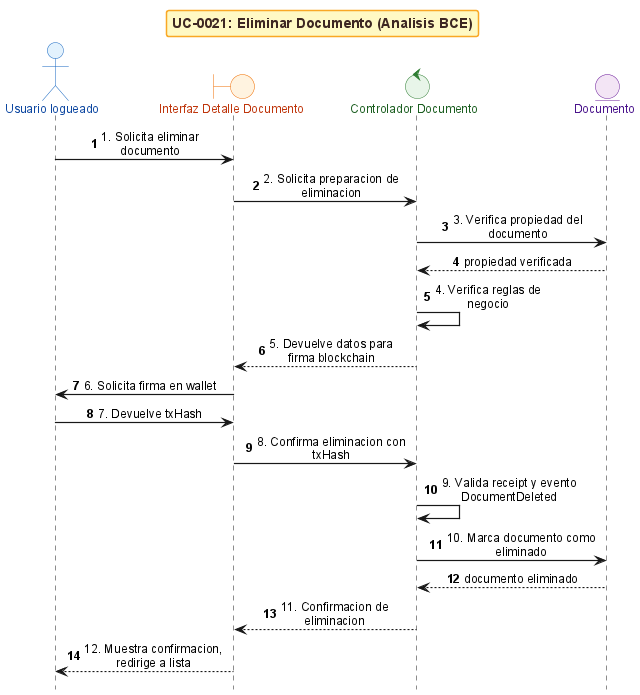
\includegraphics[width=0.92\textwidth]{diagramas/seq-bce-uc0021-delete.png}\caption{Análisis BCE — UC-0021: Eliminar Documento}\label{fig:seq-bce-uc0021}\end{figure}
\begin{figure}[H]\centering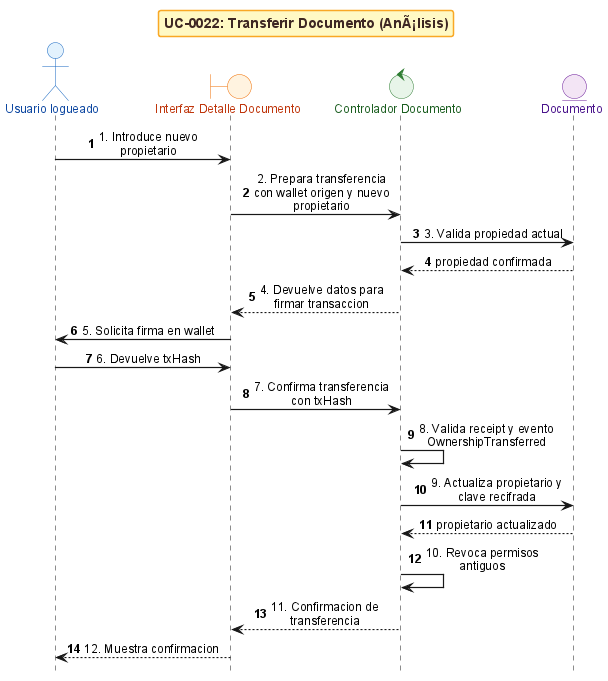
\includegraphics[width=0.92\textwidth]{diagramas/seq-bce-uc0022-transfer.png}\caption{Análisis BCE — UC-0022: Transferir Documento}\label{fig:seq-bce-uc0022}\end{figure}
\begin{figure}[H]\centering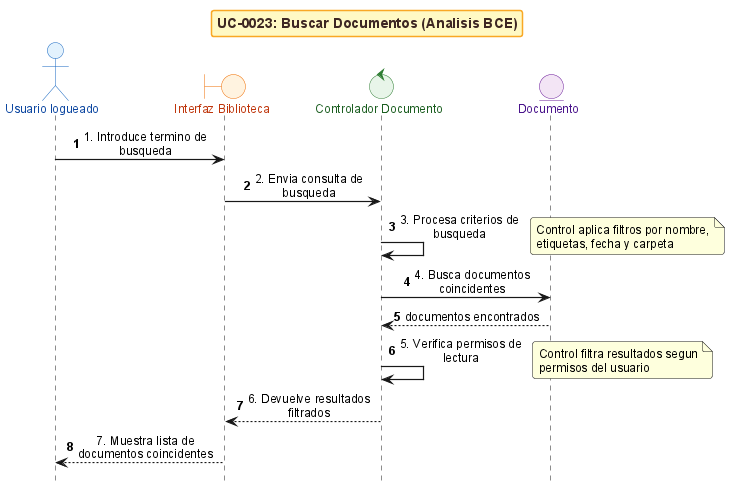
\includegraphics[width=0.90\textwidth]{diagramas/seq-bce-uc0023-search.png}\caption{Análisis BCE — UC-0023: Buscar Documentos}\label{fig:seq-bce-uc0023}\end{figure}
\begin{figure}[H]\centering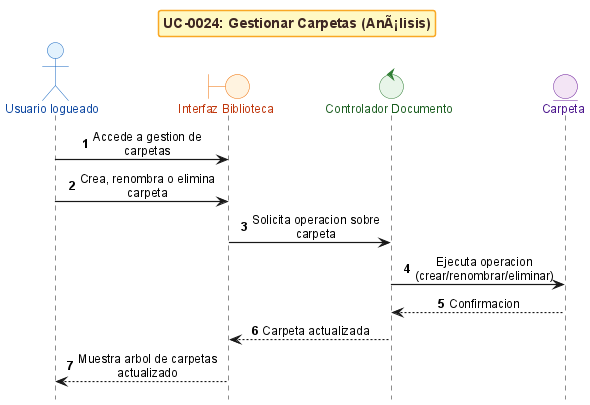
\includegraphics[width=0.90\textwidth]{diagramas/seq-bce-uc0024-manage-folders.png}\caption{Análisis BCE — UC-0024: Gestionar Carpetas}\label{fig:seq-bce-uc0024}\end{figure}
\begin{figure}[H]\centering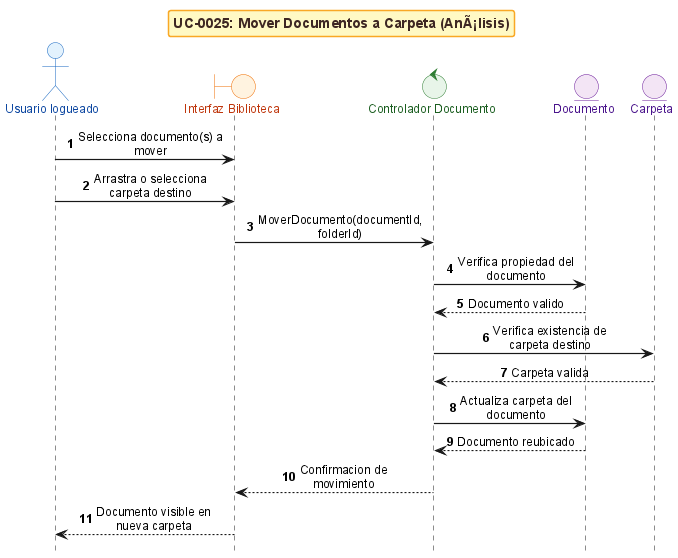
\includegraphics[width=0.90\textwidth]{diagramas/seq-bce-uc0025-move-documents.png}\caption{Análisis BCE — UC-0025: Mover Documentos}\label{fig:seq-bce-uc0025}\end{figure}

\subsection{Paquete: Versionado (UC-0026 a UC-0030)}

\begin{figure}[H]\centering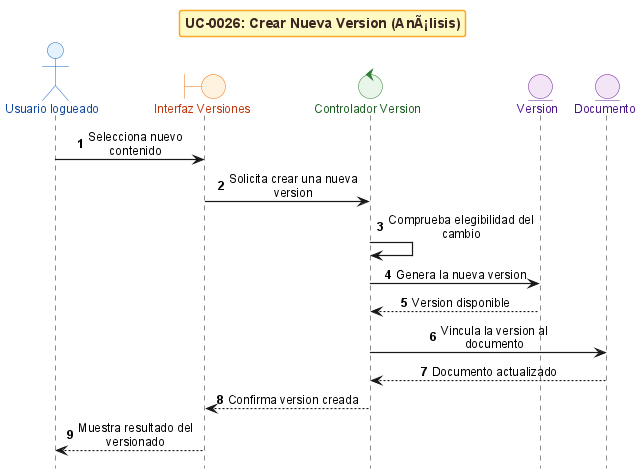
\includegraphics[width=0.92\textwidth]{diagramas/seq-bce-uc0026-version.png}\caption{Análisis BCE — UC-0026: Crear Nueva Versión}\label{fig:seq-bce-uc0026}\end{figure}
\begin{figure}[H]\centering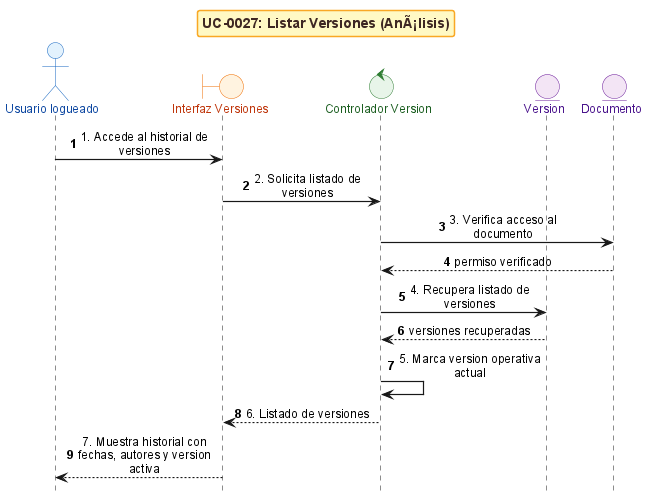
\includegraphics[width=0.88\textwidth]{diagramas/seq-bce-uc0027-list-versions.png}\caption{Análisis BCE — UC-0027: Listar Versiones}\label{fig:seq-bce-uc0027}\end{figure}
\begin{figure}[H]\centering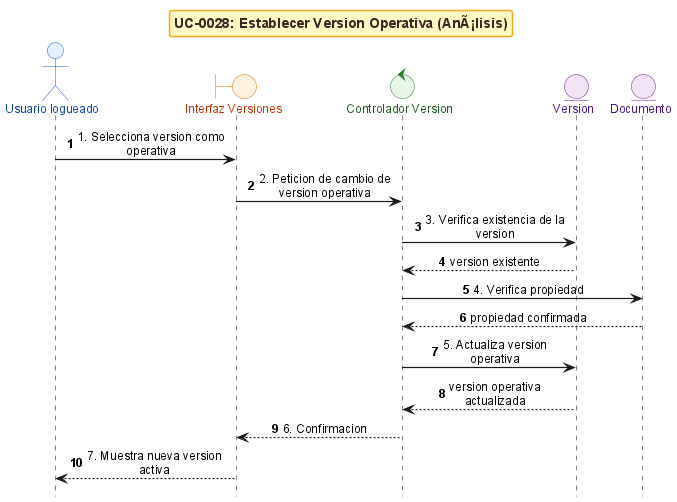
\includegraphics[width=0.92\textwidth]{diagramas/seq-bce-uc0028-operational.png}\caption{Análisis BCE — UC-0028: Establecer Versión Operativa}\label{fig:seq-bce-uc0028}\end{figure}
\begin{figure}[H]\centering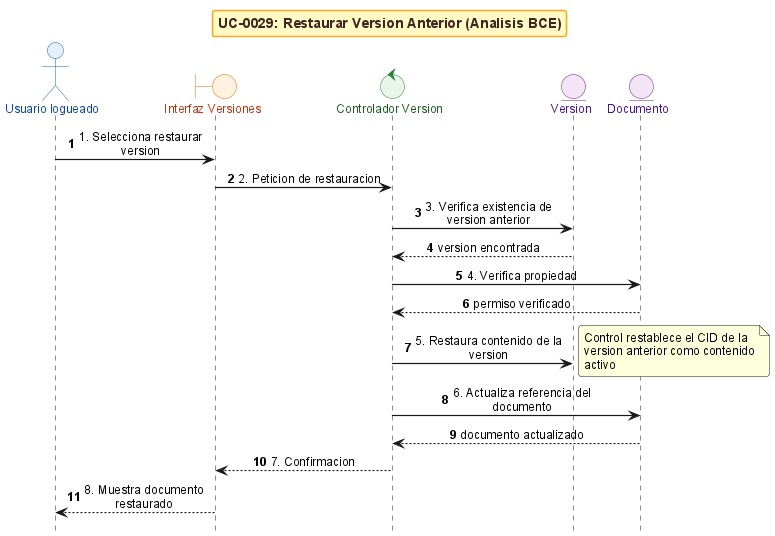
\includegraphics[width=0.92\textwidth]{diagramas/seq-bce-uc0029-restore.png}\caption{Análisis BCE — UC-0029: Restaurar Versión}\label{fig:seq-bce-uc0029}\end{figure}
\begin{figure}[H]\centering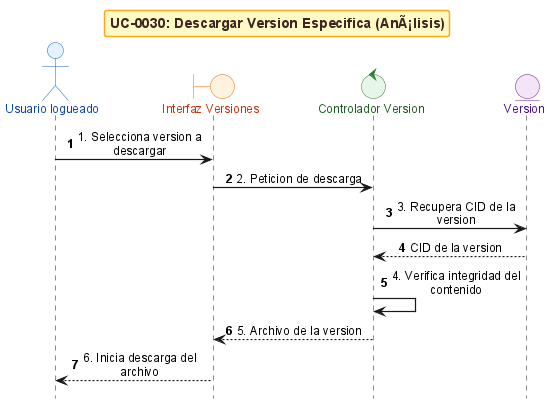
\includegraphics[width=0.90\textwidth]{diagramas/seq-bce-uc0030-download-version.png}\caption{Análisis BCE — UC-0030: Descargar Versión}\label{fig:seq-bce-uc0030}\end{figure}

\subsection{Paquete: Firmas (UC-0031 a UC-0033)}

\begin{figure}[H]\centering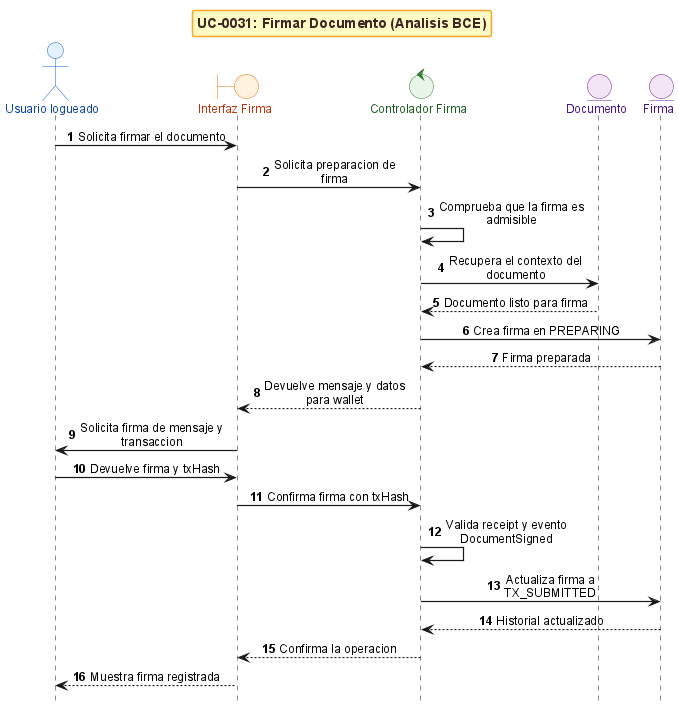
\includegraphics[width=0.92\textwidth]{diagramas/seq-bce-uc0031-sign.png}\caption{Análisis BCE — UC-0031: Firmar Documento}\label{fig:seq-bce-uc0031}\end{figure}
\begin{figure}[H]\centering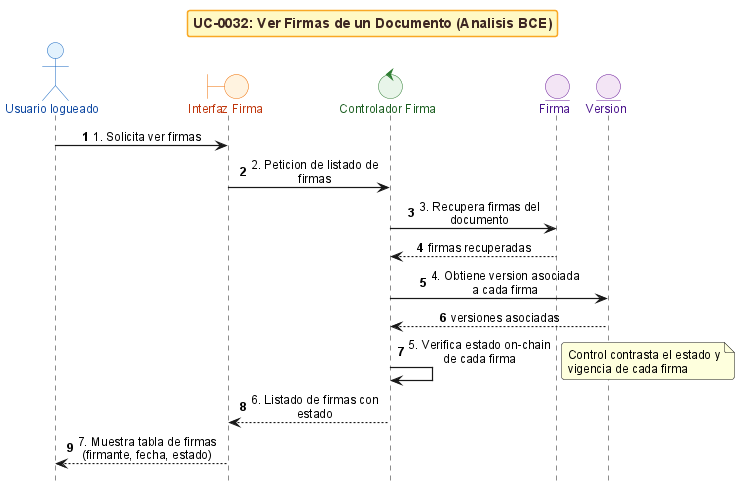
\includegraphics[width=0.92\textwidth]{diagramas/seq-bce-uc0032-view-signatures.png}\caption{Análisis BCE — UC-0032: Ver Firmas}\label{fig:seq-bce-uc0032}\end{figure}
\begin{figure}[H]\centering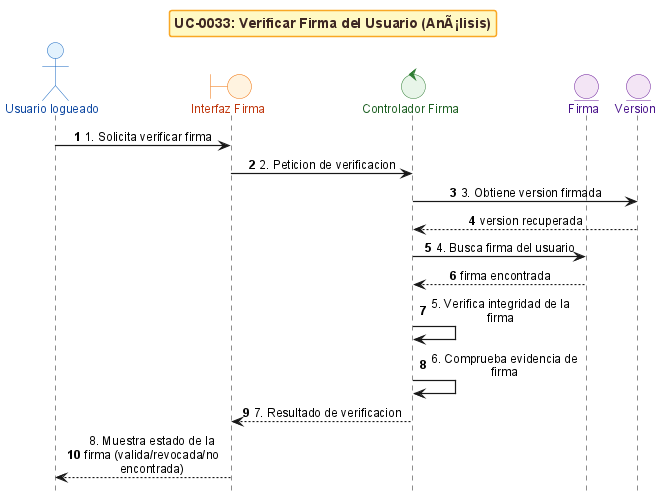
\includegraphics[width=0.92\textwidth]{diagramas/seq-bce-uc0033-verify-signature.png}\caption{Análisis BCE — UC-0033: Verificar Firma}\label{fig:seq-bce-uc0033}\end{figure}

\subsection{Paquete: Compartición (UC-0034 a UC-0036)}

\begin{figure}[H]\centering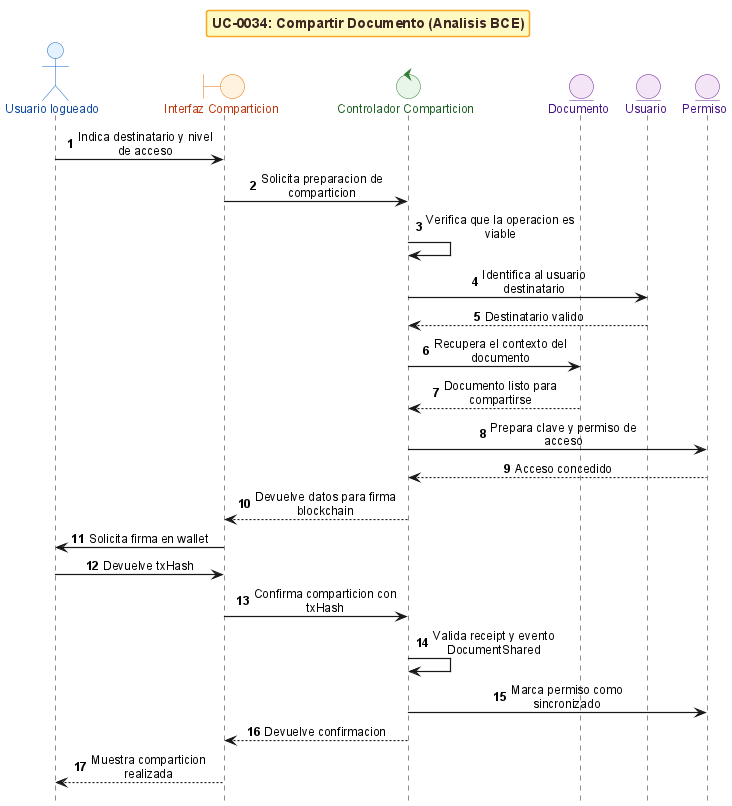
\includegraphics[width=0.92\textwidth]{diagramas/seq-bce-uc0034-share.png}\caption{Análisis BCE — UC-0034: Compartir Documento}\label{fig:seq-bce-uc0034}\end{figure}
\begin{figure}[H]\centering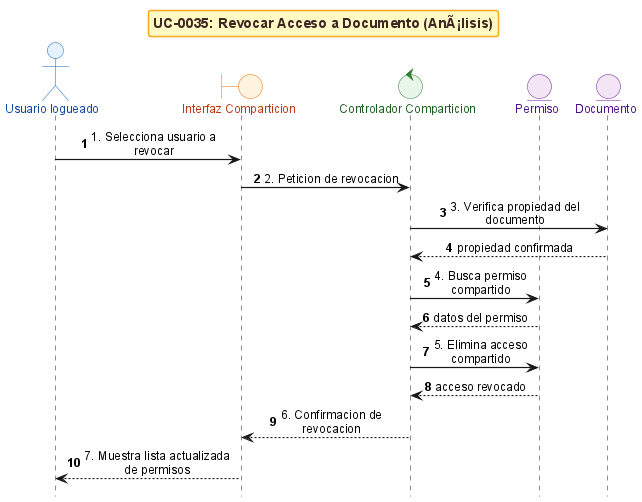
\includegraphics[width=0.92\textwidth]{diagramas/seq-bce-uc0035-revoke.png}\caption{Análisis BCE — UC-0035: Revocar Acceso}\label{fig:seq-bce-uc0035}\end{figure}
\begin{figure}[H]\centering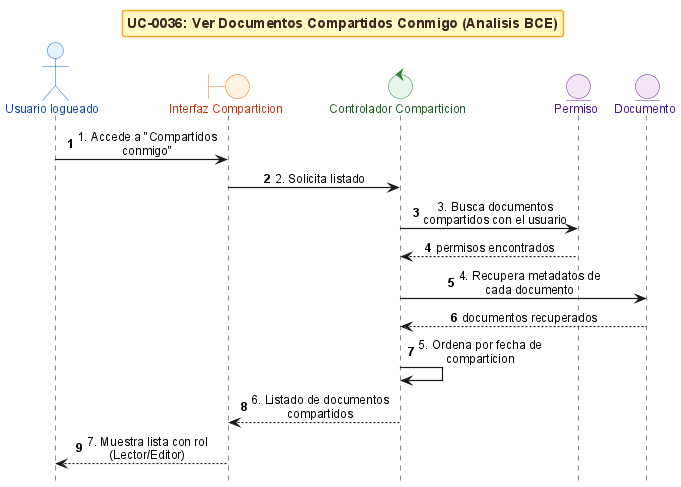
\includegraphics[width=0.92\textwidth]{diagramas/seq-bce-uc0036-shared-with-me.png}\caption{Análisis BCE — UC-0036: Compartidos Conmigo}\label{fig:seq-bce-uc0036}\end{figure}

\subsection{Paquete: Auditoría y verificación (UC-0037 a UC-0041)}

\begin{figure}[H]\centering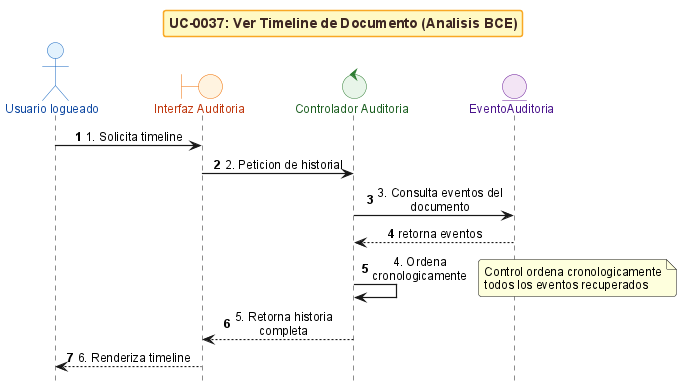
\includegraphics[width=0.92\textwidth]{diagramas/seq-bce-uc0037-timeline.png}\caption{Análisis BCE — UC-0037: Timeline del Documento}\label{fig:seq-bce-uc0037}\end{figure}
\begin{figure}[H]\centering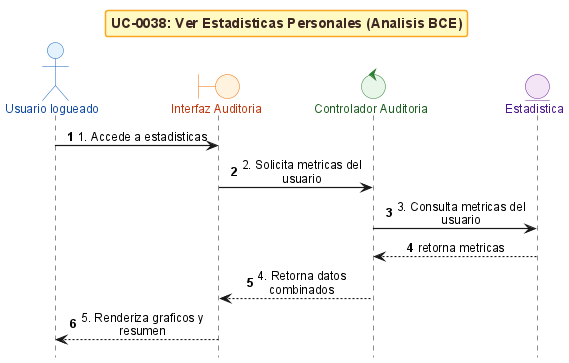
\includegraphics[width=0.92\textwidth]{diagramas/seq-bce-uc0038-stats.png}\caption{Análisis BCE — UC-0038: Estadísticas Personales}\label{fig:seq-bce-uc0038}\end{figure}
\begin{figure}[H]\centering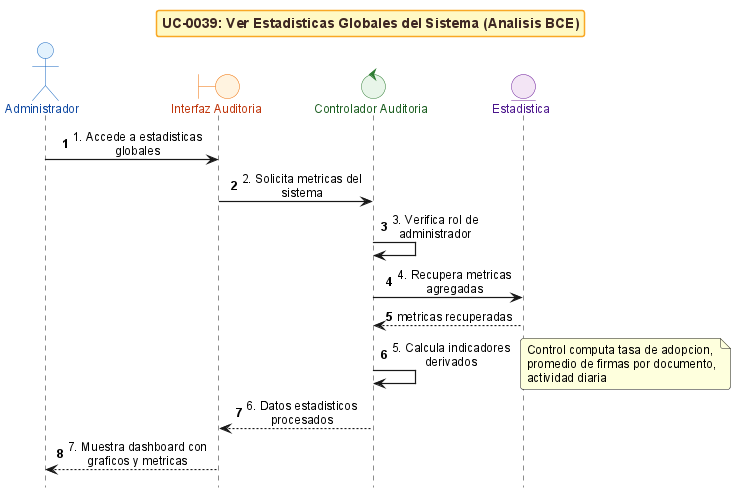
\includegraphics[width=0.92\textwidth]{diagramas/seq-bce-uc0039-global-stats.png}\caption{Análisis BCE — UC-0039: Estadísticas Globales}\label{fig:seq-bce-uc0039}\end{figure}
\begin{figure}[H]\centering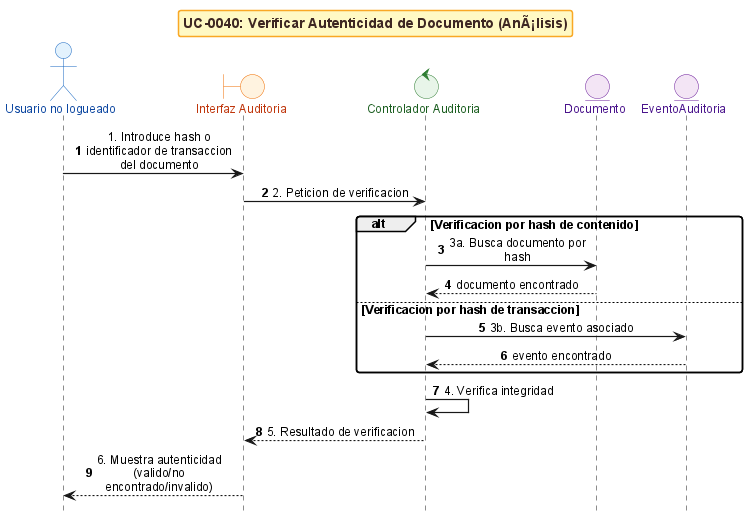
\includegraphics[width=0.92\textwidth]{diagramas/seq-bce-uc0040-verify-authenticity.png}\caption{Análisis BCE — UC-0040: Verificar Autenticidad}\label{fig:seq-bce-uc0040}\end{figure}
\begin{figure}[H]\centering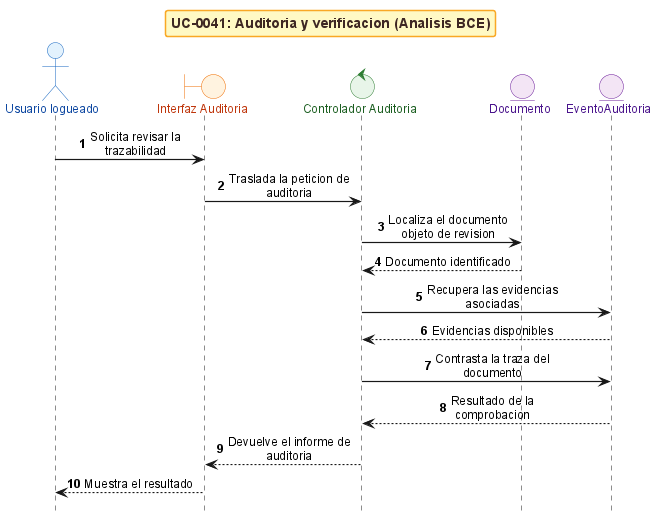
\includegraphics[width=0.92\textwidth]{diagramas/seq-bce-uc0041-audit.png}\caption{Análisis BCE — UC-0041: Auditoría Blockchain}\label{fig:seq-bce-uc0041}\end{figure}

\subsection{Paquete: Administración (UC-0042 a UC-0043)}

\begin{figure}[H]\centering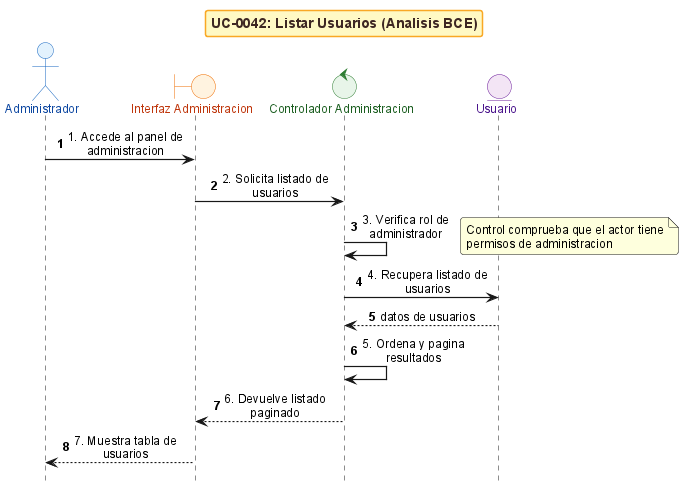
\includegraphics[width=0.88\textwidth]{diagramas/seq-bce-uc0042-list-users.png}\caption{Análisis BCE — UC-0042: Listar Usuarios}\label{fig:seq-bce-uc0042}\end{figure}
\begin{figure}[H]\centering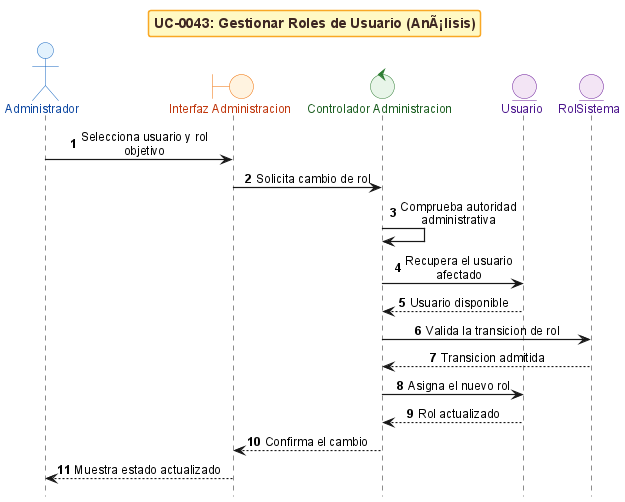
\includegraphics[width=0.90\textwidth]{diagramas/seq-bce-uc0043-manage-roles.png}\caption{Análisis BCE — UC-0043: Gestionar Roles}\label{fig:seq-bce-uc0043}\end{figure}


% ============================================================
% PARTE B — DISEÑO ARQUITECTÓNICO Y PROCEDIMENTAL
% ============================================================

\section{Arquitectura del sistema}

La arquitectura de DocumentChain se organiza en capas funcionales desacopladas. El frontend (React 19 + Vite) consume la API REST del backend (Express 4 + Prisma), que coordina tres capas de persistencia: PostgreSQL para el estado relacional, IPFS (Pinata por defecto, Kubo opcional) para el contenido documental, y una red Ethereum local (Hardhat) para el registro inmutable de operaciones. La Figura~\ref{fig:arquitectura} presenta la vista de capas del sistema.

\begin{figure}[H]
    \centering
    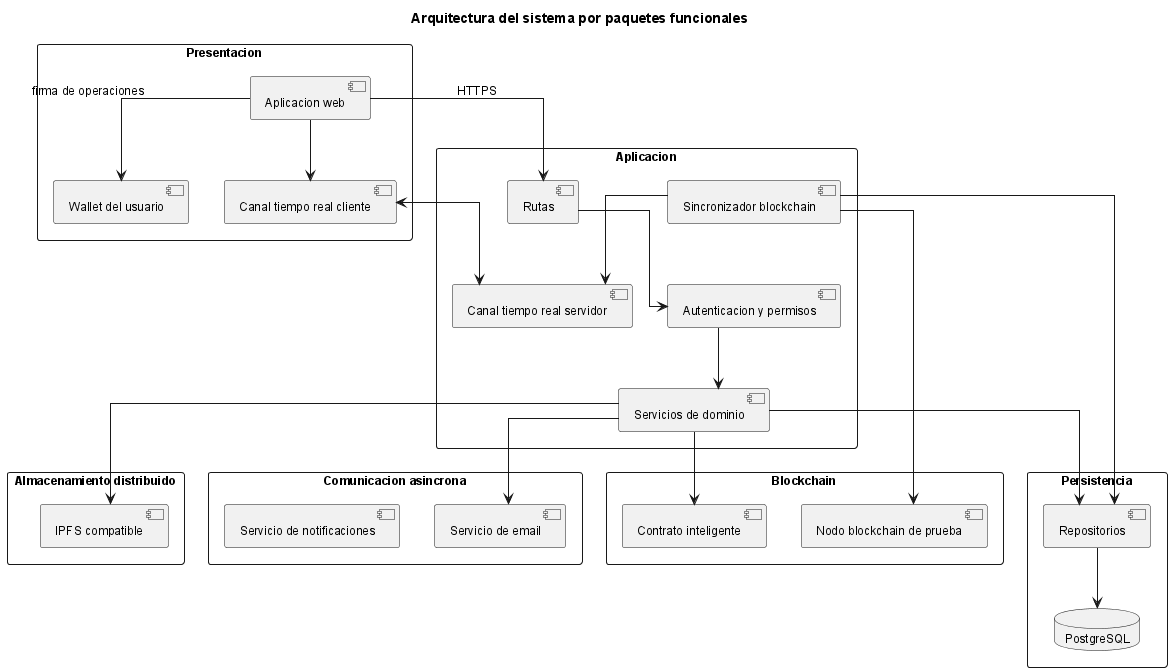
\includegraphics[width=0.95\linewidth]{diagramas/arquitectura.png}
    \caption{Arquitectura del sistema DocumentChain}
    \label{fig:arquitectura}
\end{figure}

\section{Patrones de diseño}

\subsection{Patrón prepare/confirm}

Las operaciones que requieren registro en blockchain siguen el patrón prepare/confirm. En la fase \textit{prepare} el backend valida permisos, procesa el contenido y crea un registro en estado \texttt{PREPARING}. En la fase \textit{confirm} el usuario firma la transacción con su wallet, el backend valida el receipt on-chain verificando el evento esperado, y actualiza el estado a \texttt{TX\_SUBMITTED}. Un proceso de sincronización periódica confirma los bloques y transiciona a \texttt{SYNCED}. La Figura~\ref{fig:prepare-confirm} muestra el flujo de estados de este patrón.

\begin{figure}[H]
    \centering
    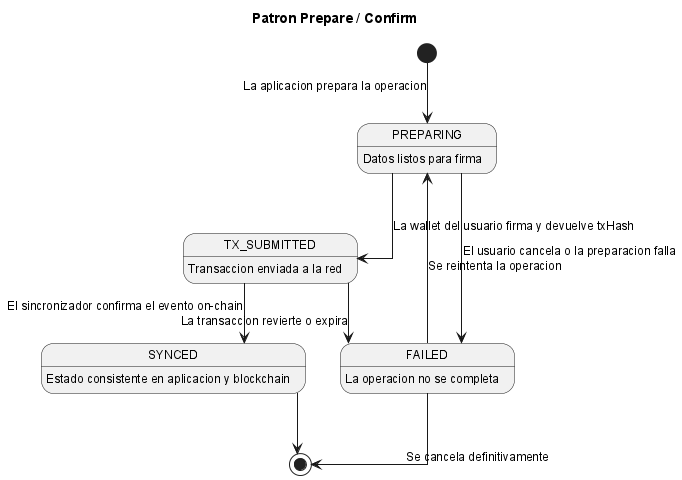
\includegraphics[width=0.9\textwidth]{diagramas/prepare-confirm.png}
    \caption{Patrón prepare/confirm y estados de sincronización}
    \label{fig:prepare-confirm}
\end{figure}

\subsection{Ciclo de vida del documento}

La Figura~\ref{fig:state-lifecycle} recoge los estados por los que transita un documento desde su creación hasta su borrado lógico, incluyendo las transiciones de archivado y los estados de sincronización blockchain.

\begin{figure}[H]
    \centering
    
\includegraphics[width=0.92\textwidth]{diagramas/state-document-lifecycle.png}
    \caption{Ciclo de vida del documento}
    \label{fig:state-lifecycle}
\end{figure}

\section{Subsistemas de diseño}

\subsection{Diagrama de paquetes}

La Figura~\ref{fig:package} descompone el sistema en paquetes funcionales: frontend, backend, smart contracts e infraestructura, mostrando las dependencias entre ellos.

\begin{figure}[H]
    \centering
    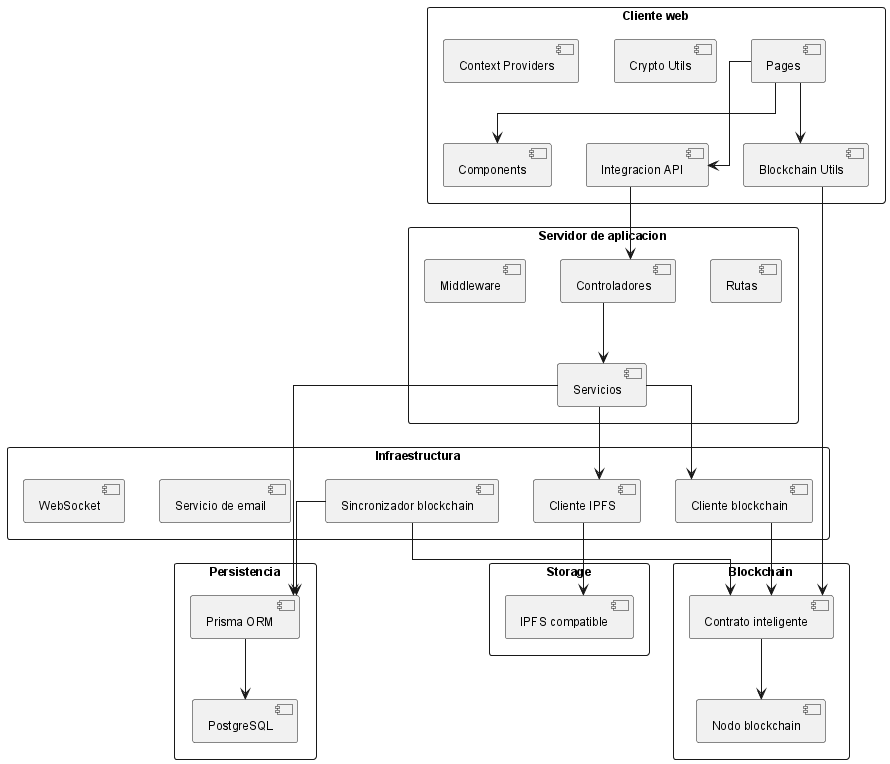
\includegraphics[width=0.9\textwidth]{diagramas/package-diagram.png}
    \caption{Diagrama de paquetes del sistema}
    \label{fig:package}
\end{figure}

\subsection{Diagrama de componentes}

La Figura~\ref{fig:components} detalla los componentes principales de cada capa y sus interfaces de comunicación: API REST entre frontend y backend, JSON-RPC para la interacción con el nodo blockchain, y el protocolo IPFS para el almacenamiento de contenido.

\begin{figure}[H]
    \centering
    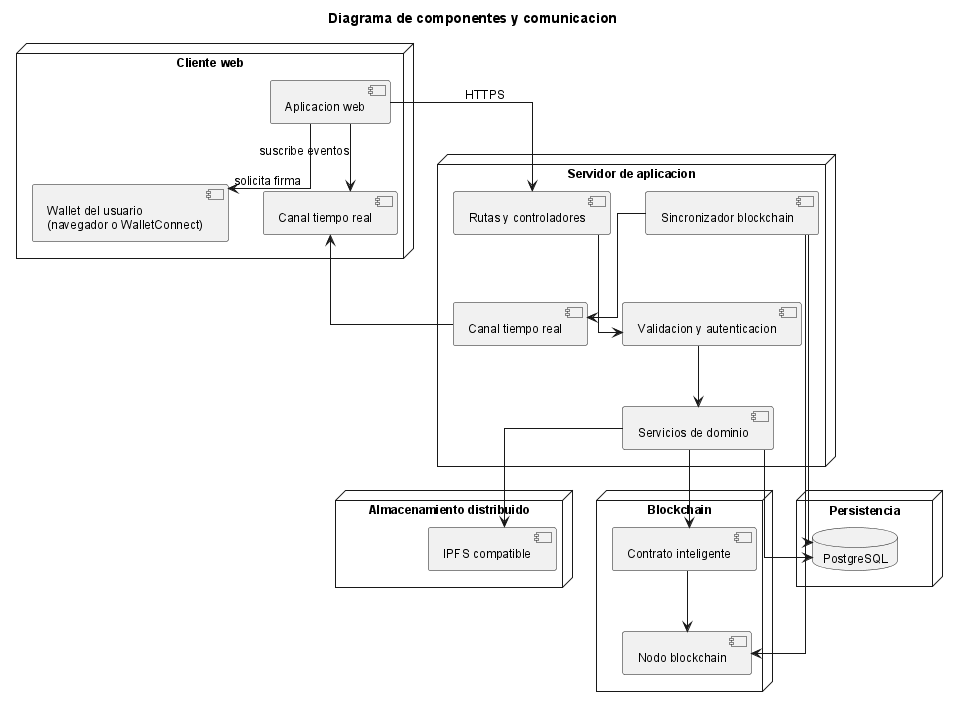
\includegraphics[width=0.76\linewidth]{diagramas/components.png}
    \caption{Diagrama de componentes}
    \label{fig:components}
\end{figure}

\subsection{Clases de diseño}

La Figura~\ref{fig:class-design} presenta el diagrama de clases de diseño, donde se reflejan las clases del backend con sus atributos y métodos principales, las relaciones de herencia y composición, y los servicios que coordinan la lógica de negocio.

\begin{figure}[H]
    \centering
    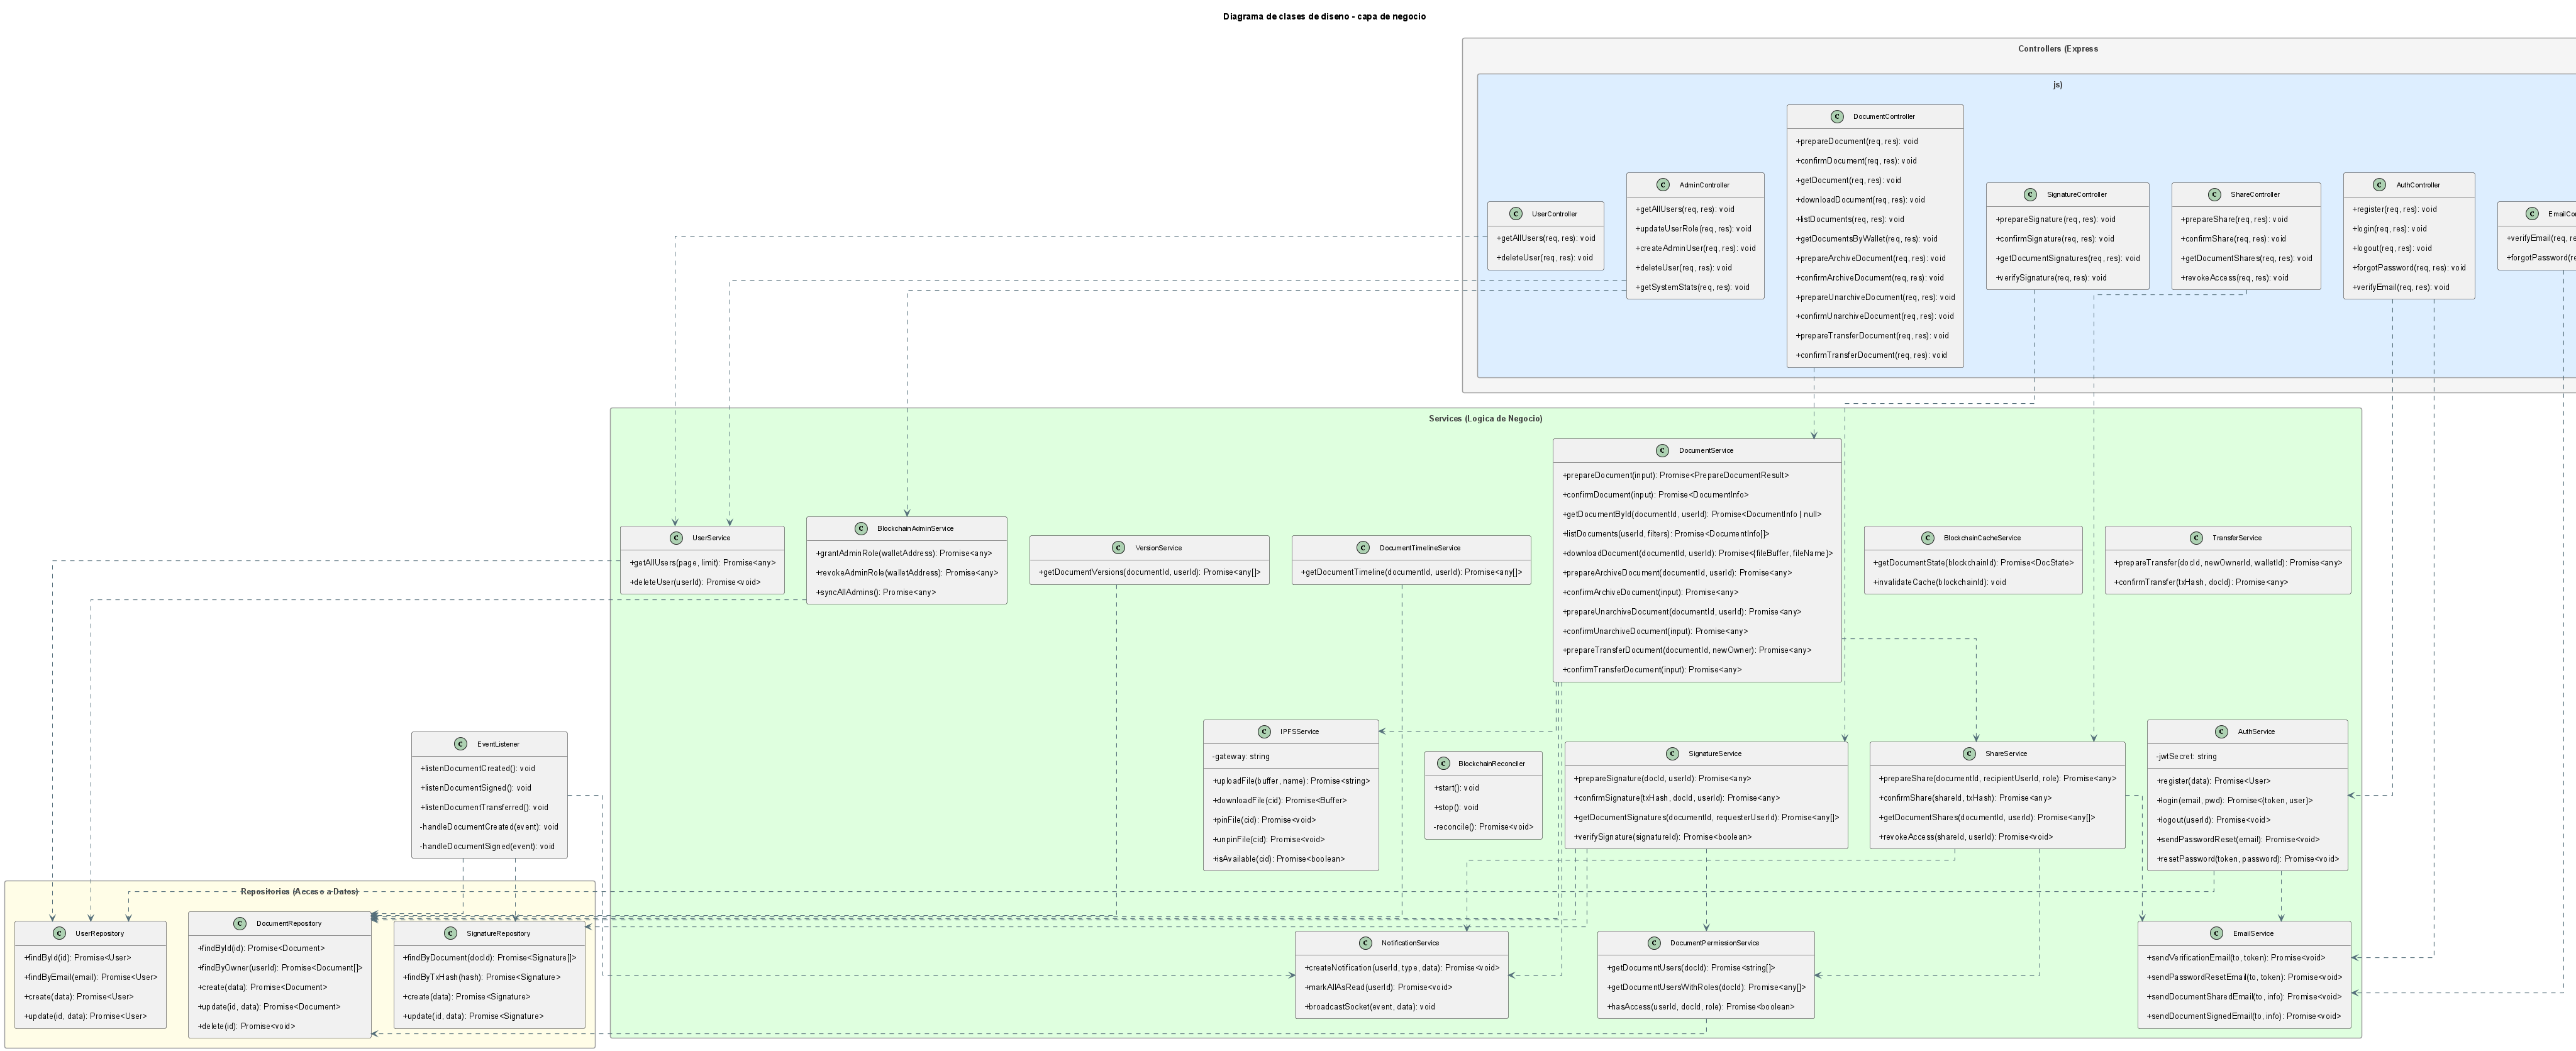
\includegraphics[width=0.95\linewidth]{diagramas/class-design.png}
    \caption{Diagrama de clases de diseño}
    \label{fig:class-design}
\end{figure}


\section{Diagramas de secuencia de diseño}

Los diagramas de secuencia de diseño muestran la implementación real de cada caso de uso, con los componentes técnicos del sistema: páginas React, endpoints REST, servicios del backend, capa de acceso a datos, adaptador IPFS y el contrato \texttt{DocumentRegistry}. A diferencia de los diagramas BCE de análisis, aquí cada objeto representa una clase o componente concreto del código.

\subsection{Gestión de cuenta y acceso}

\begin{figure}[H]\centering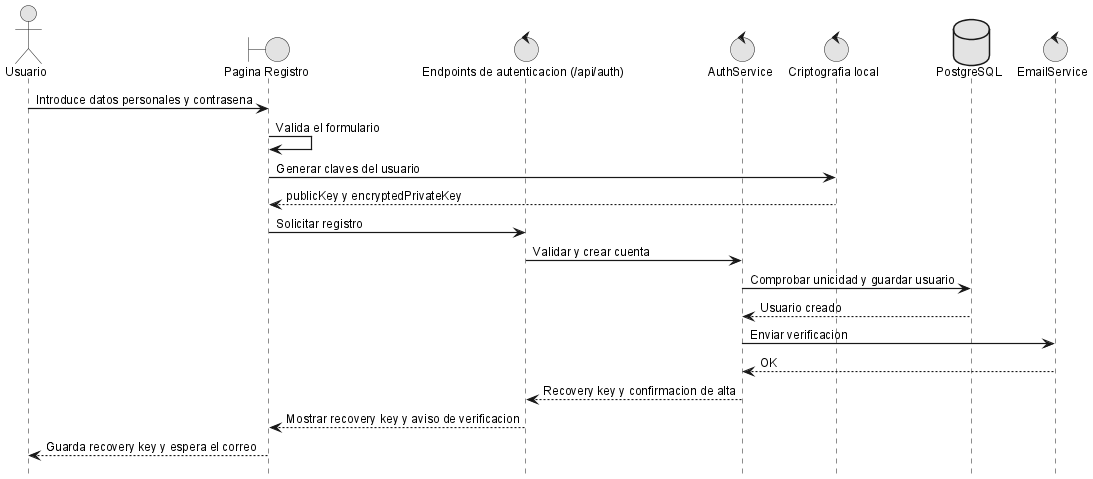
\includegraphics[width=0.9\textwidth]{diagramas/seq-register.png}\caption{Secuencia de diseño — UC-0001: Registrar Usuario}\label{fig:seq-register}\end{figure}
\begin{figure}[H]\centering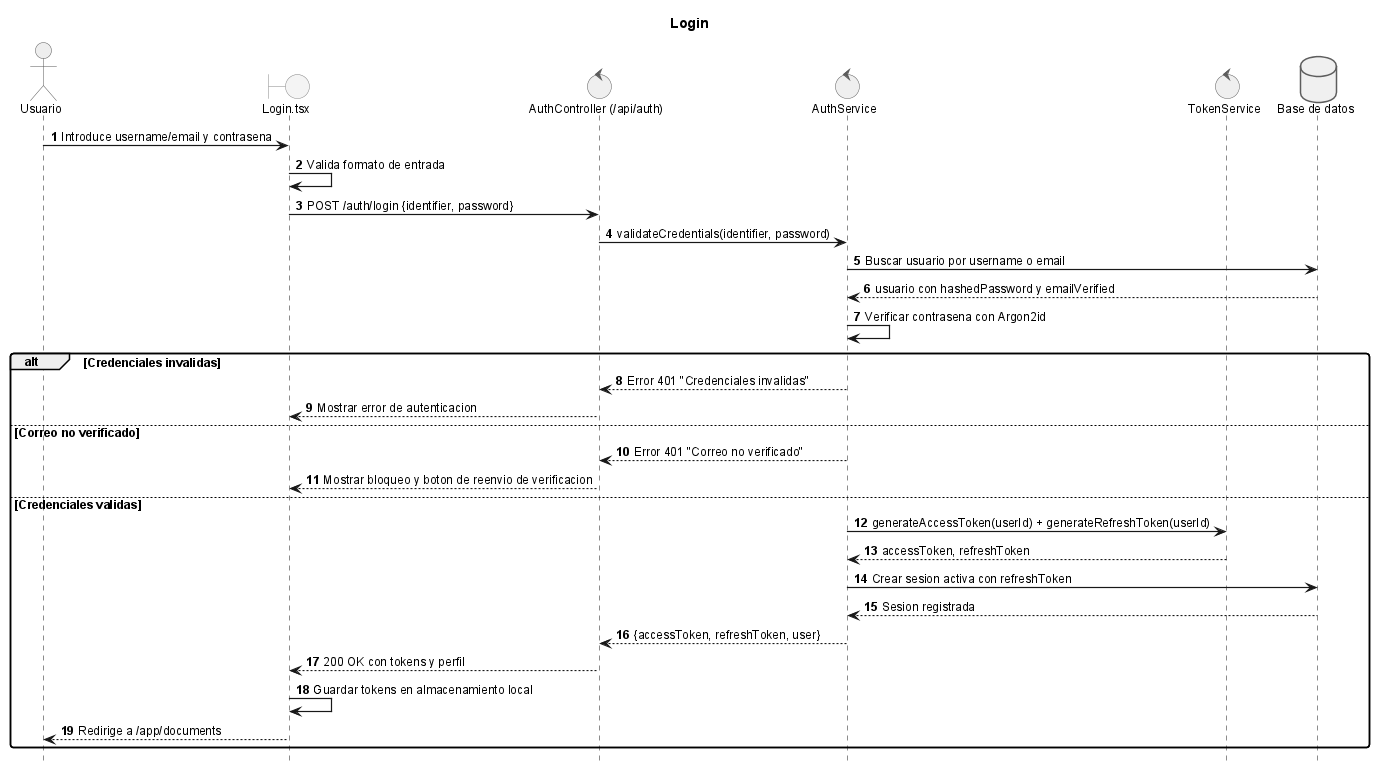
\includegraphics[width=0.9\textwidth]{diagramas/seq-login.png}\caption{Secuencia de diseño — UC-0002: Iniciar Sesión}\label{fig:seq-login}\end{figure}
\begin{figure}[H]\centering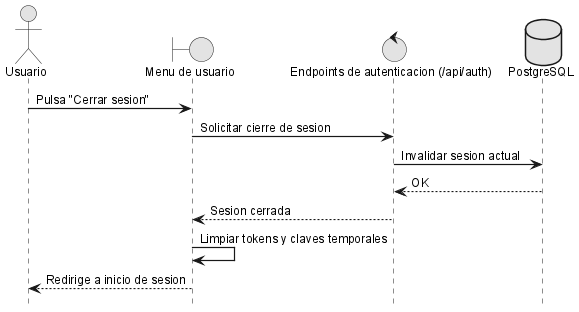
\includegraphics[width=0.9\textwidth]{diagramas/seq-logout.png}\caption{Secuencia de diseño — UC-0003: Cerrar Sesión}\label{fig:seq-logout}\end{figure}
\begin{figure}[H]\centering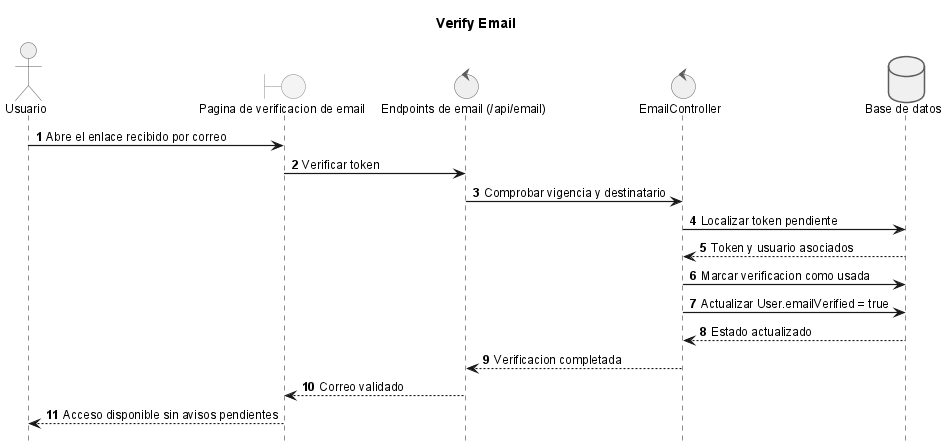
\includegraphics[width=0.9\textwidth]{diagramas/seq-verify-email.png}\caption{Secuencia de diseño — UC-0013: Verificar Email}\label{fig:seq-verify-email}\end{figure}
\begin{figure}[H]\centering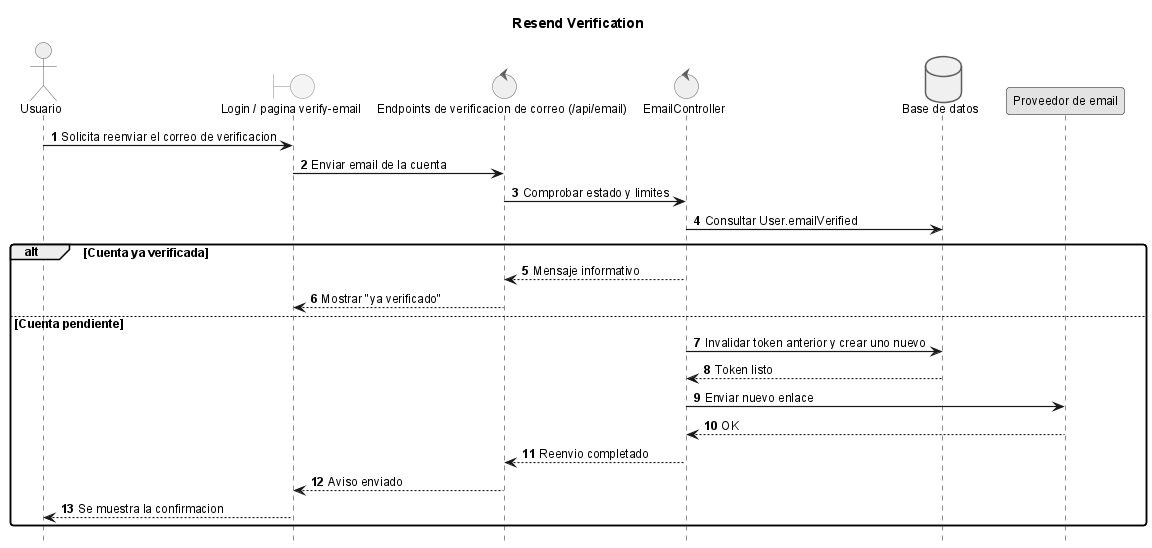
\includegraphics[width=0.9\textwidth]{diagramas/seq-resend-verification.png}\caption{Secuencia de diseño — UC-0014: Reenviar Verificación}\label{fig:seq-resend-verification}\end{figure}
\begin{figure}[H]\centering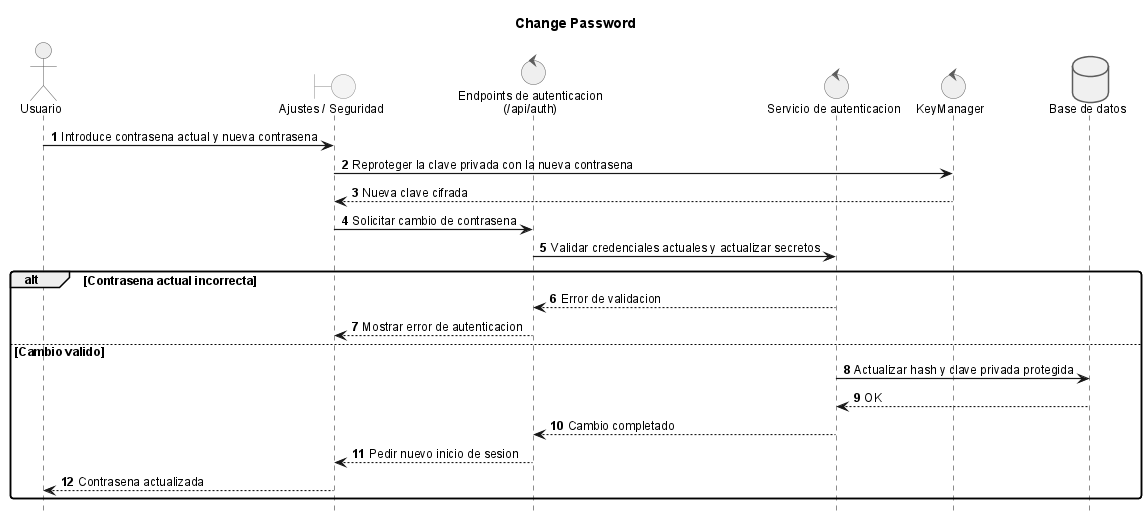
\includegraphics[width=0.9\textwidth]{diagramas/seq-change-password.png}\caption{Secuencia de diseño — UC-0011: Cambiar Contraseña}\label{fig:seq-change-password}\end{figure}
\begin{figure}[H]\centering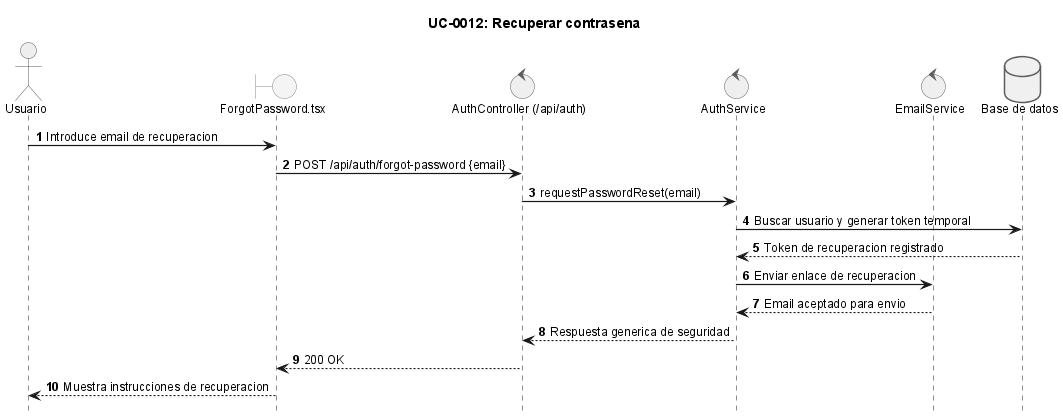
\includegraphics[width=0.9\textwidth]{diagramas/seq-recover-password.png}\caption{Secuencia de diseño — UC-0012: Recuperar Contraseña}\label{fig:seq-recover-password}\end{figure}
\begin{figure}[H]\centering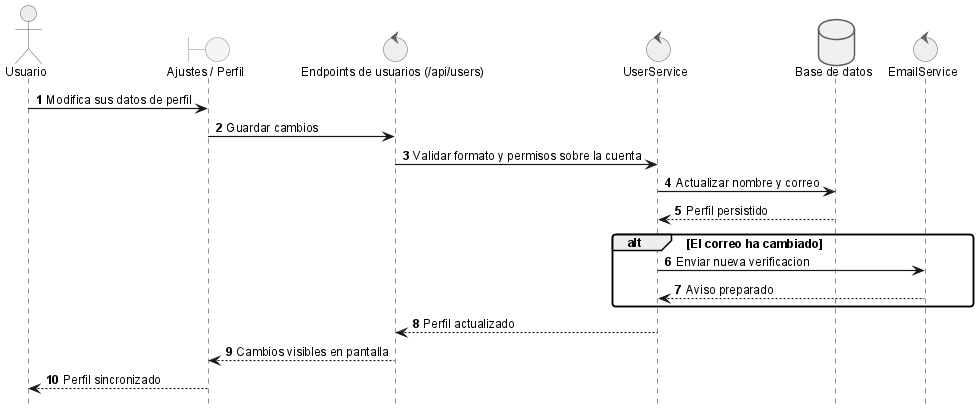
\includegraphics[width=0.9\textwidth]{diagramas/seq-profile.png}\caption{Secuencia de diseño — UC-0008: Gestionar Perfil}\label{fig:seq-profile}\end{figure}
\begin{figure}[H]\centering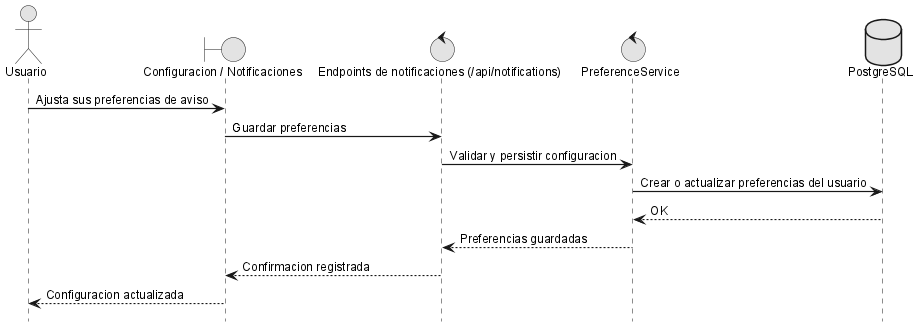
\includegraphics[width=0.9\textwidth]{diagramas/seq-preferences.png}\caption{Secuencia de diseño — Preferencias de cuenta}\label{fig:seq-preferences}\end{figure}
\begin{figure}[H]\centering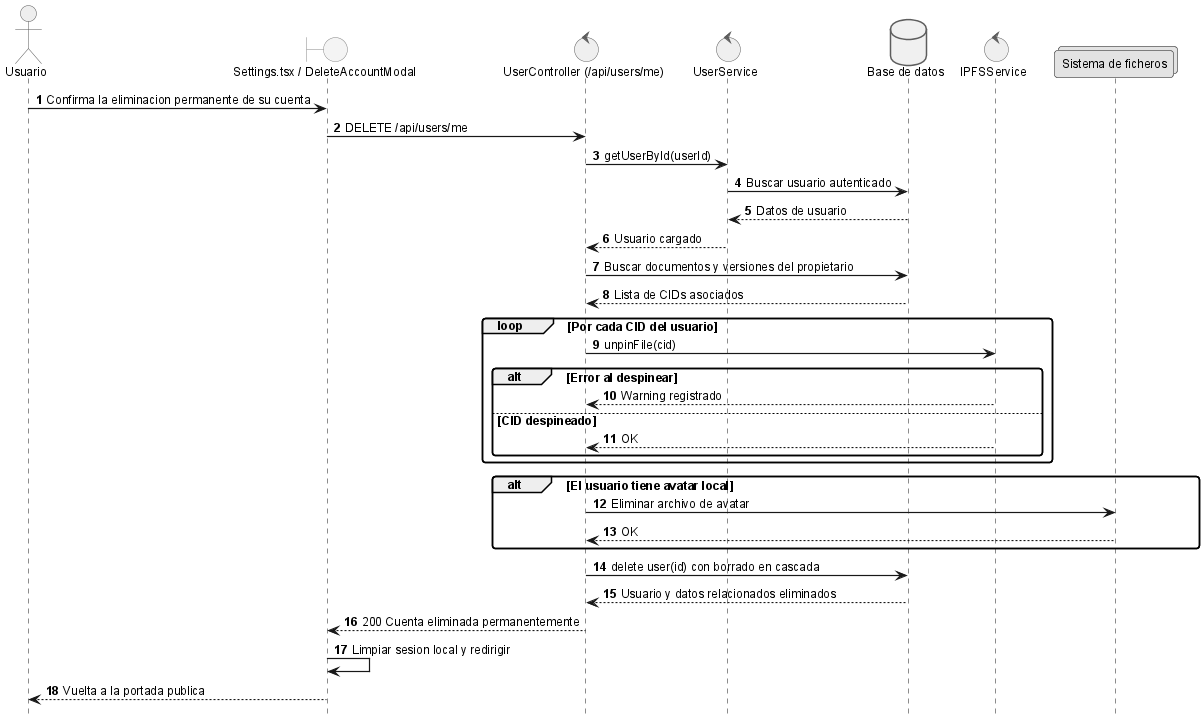
\includegraphics[width=0.9\textwidth]{diagramas/seq-delete-account.png}\caption{Secuencia de diseño — UC-0010: Eliminar Cuenta}\label{fig:seq-delete-account}\end{figure}
\begin{figure}[H]\centering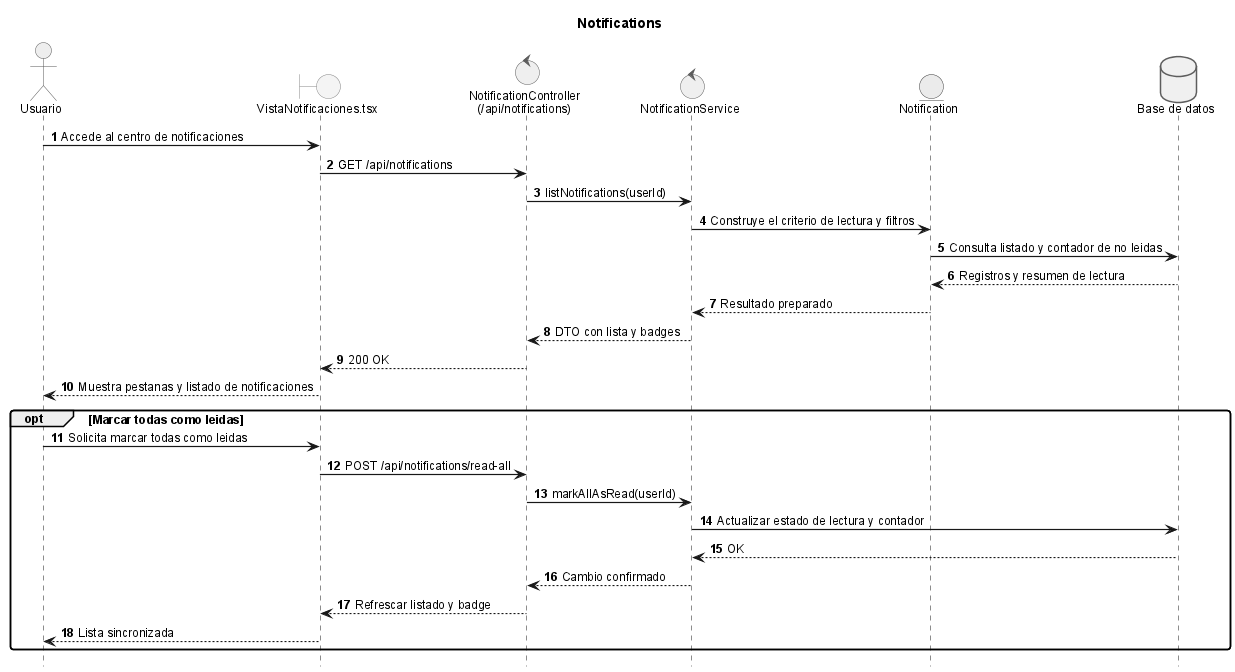
\includegraphics[width=0.9\textwidth]{diagramas/seq-notifications.png}\caption{Secuencia de diseño — UC-0009: Consultar Notificaciones}\label{fig:seq-notifications}\end{figure}

\subsection{Gestión de wallets}

\begin{figure}[H]\centering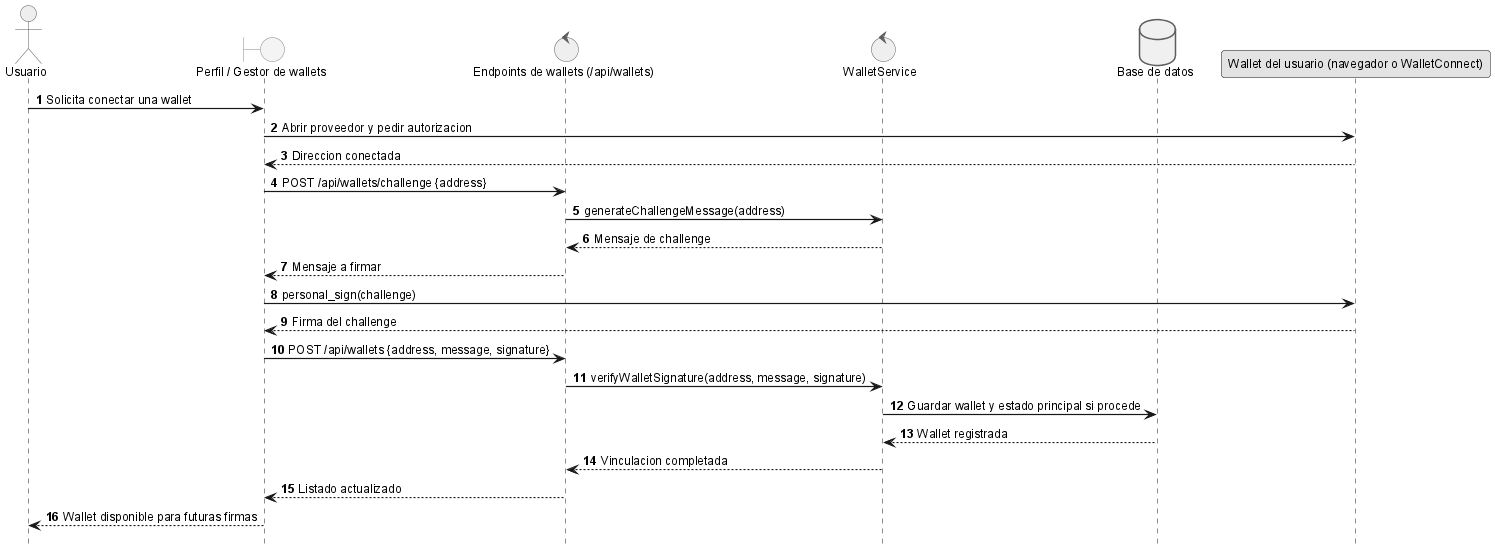
\includegraphics[width=0.9\textwidth]{diagramas/seq-connect-wallet.png}\caption{Secuencia de diseño — UC-0004: Conectar Wallet}\label{fig:seq-connect-wallet}\end{figure}
\begin{figure}[H]\centering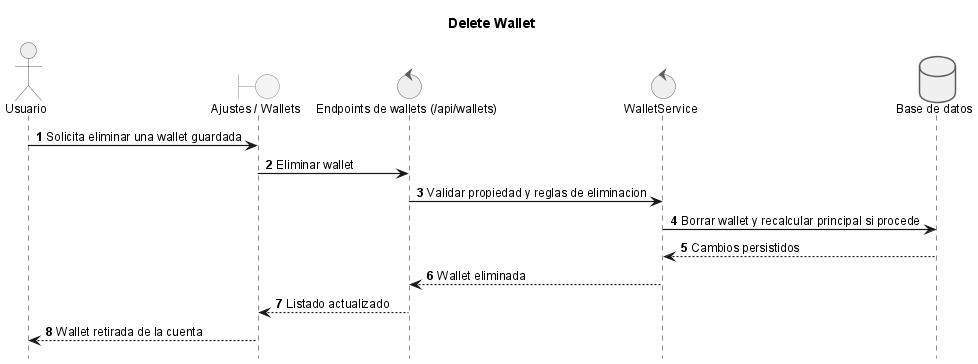
\includegraphics[width=0.9\textwidth]{diagramas/seq-delete-wallet.png}\caption{Secuencia de diseño — UC-0005: Eliminar Wallet}\label{fig:seq-delete-wallet}\end{figure}
\begin{figure}[H]\centering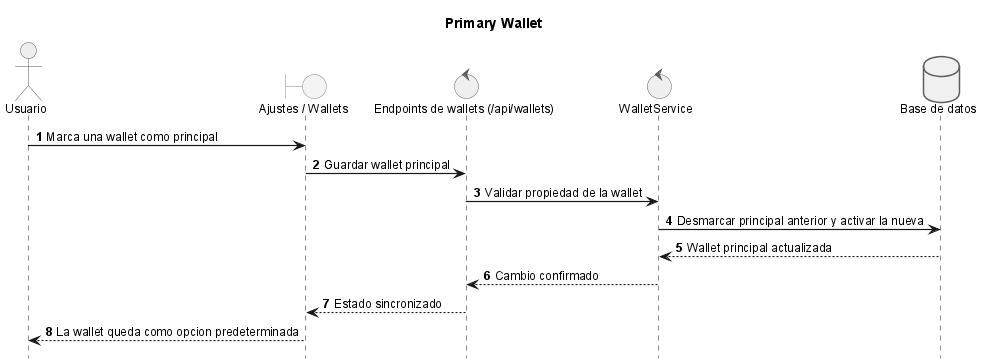
\includegraphics[width=0.9\textwidth]{diagramas/seq-primary-wallet.png}\caption{Secuencia de diseño — UC-0006: Wallet Principal}\label{fig:seq-primary-wallet}\end{figure}
\begin{figure}[H]\centering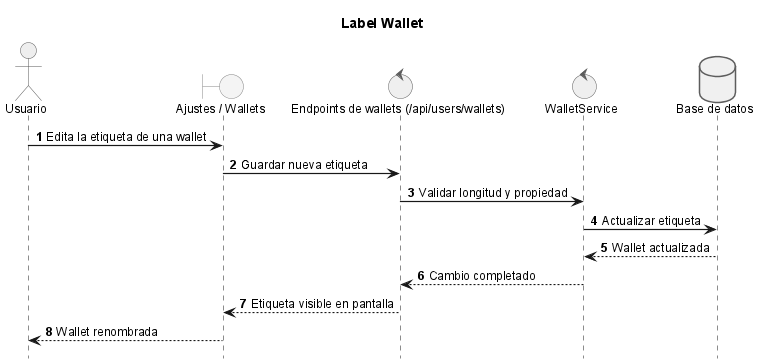
\includegraphics[width=0.9\textwidth]{diagramas/seq-label-wallet.png}\caption{Secuencia de diseño — UC-0007: Renombrar Wallet}\label{fig:seq-label-wallet}\end{figure}

\subsection{Gestión de documentos}

\begin{figure}[H]\centering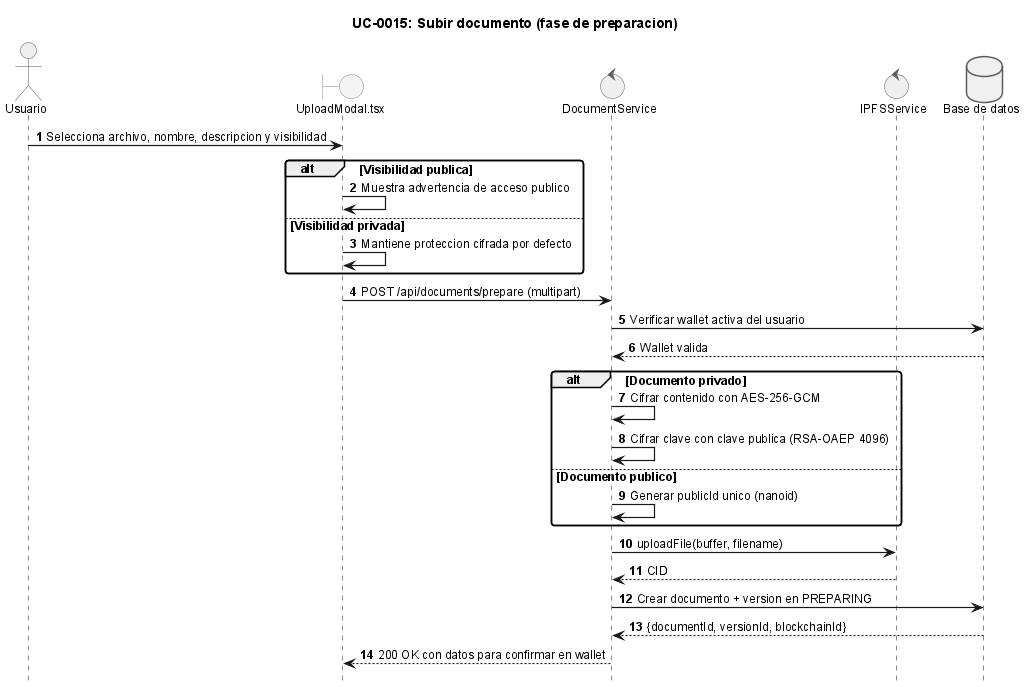
\includegraphics[width=0.9\textwidth]{diagramas/seq-upload-prepare.png}\caption{Secuencia de diseño — UC-0015: Subir Documento (prepare)}\label{fig:seq-upload-prepare}\end{figure}
\begin{figure}[H]\centering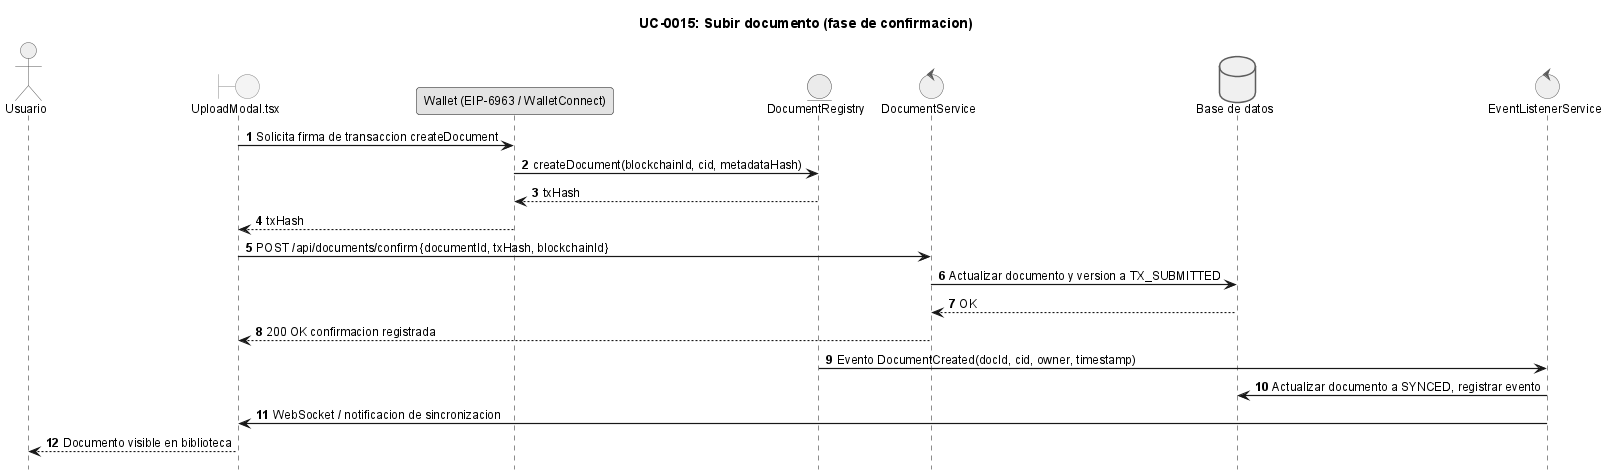
\includegraphics[width=0.9\textwidth]{diagramas/seq-upload-confirm.png}\caption{Secuencia de diseño — UC-0015: Subir Documento (confirm)}\label{fig:seq-upload-confirm}\end{figure}
\begin{figure}[H]\centering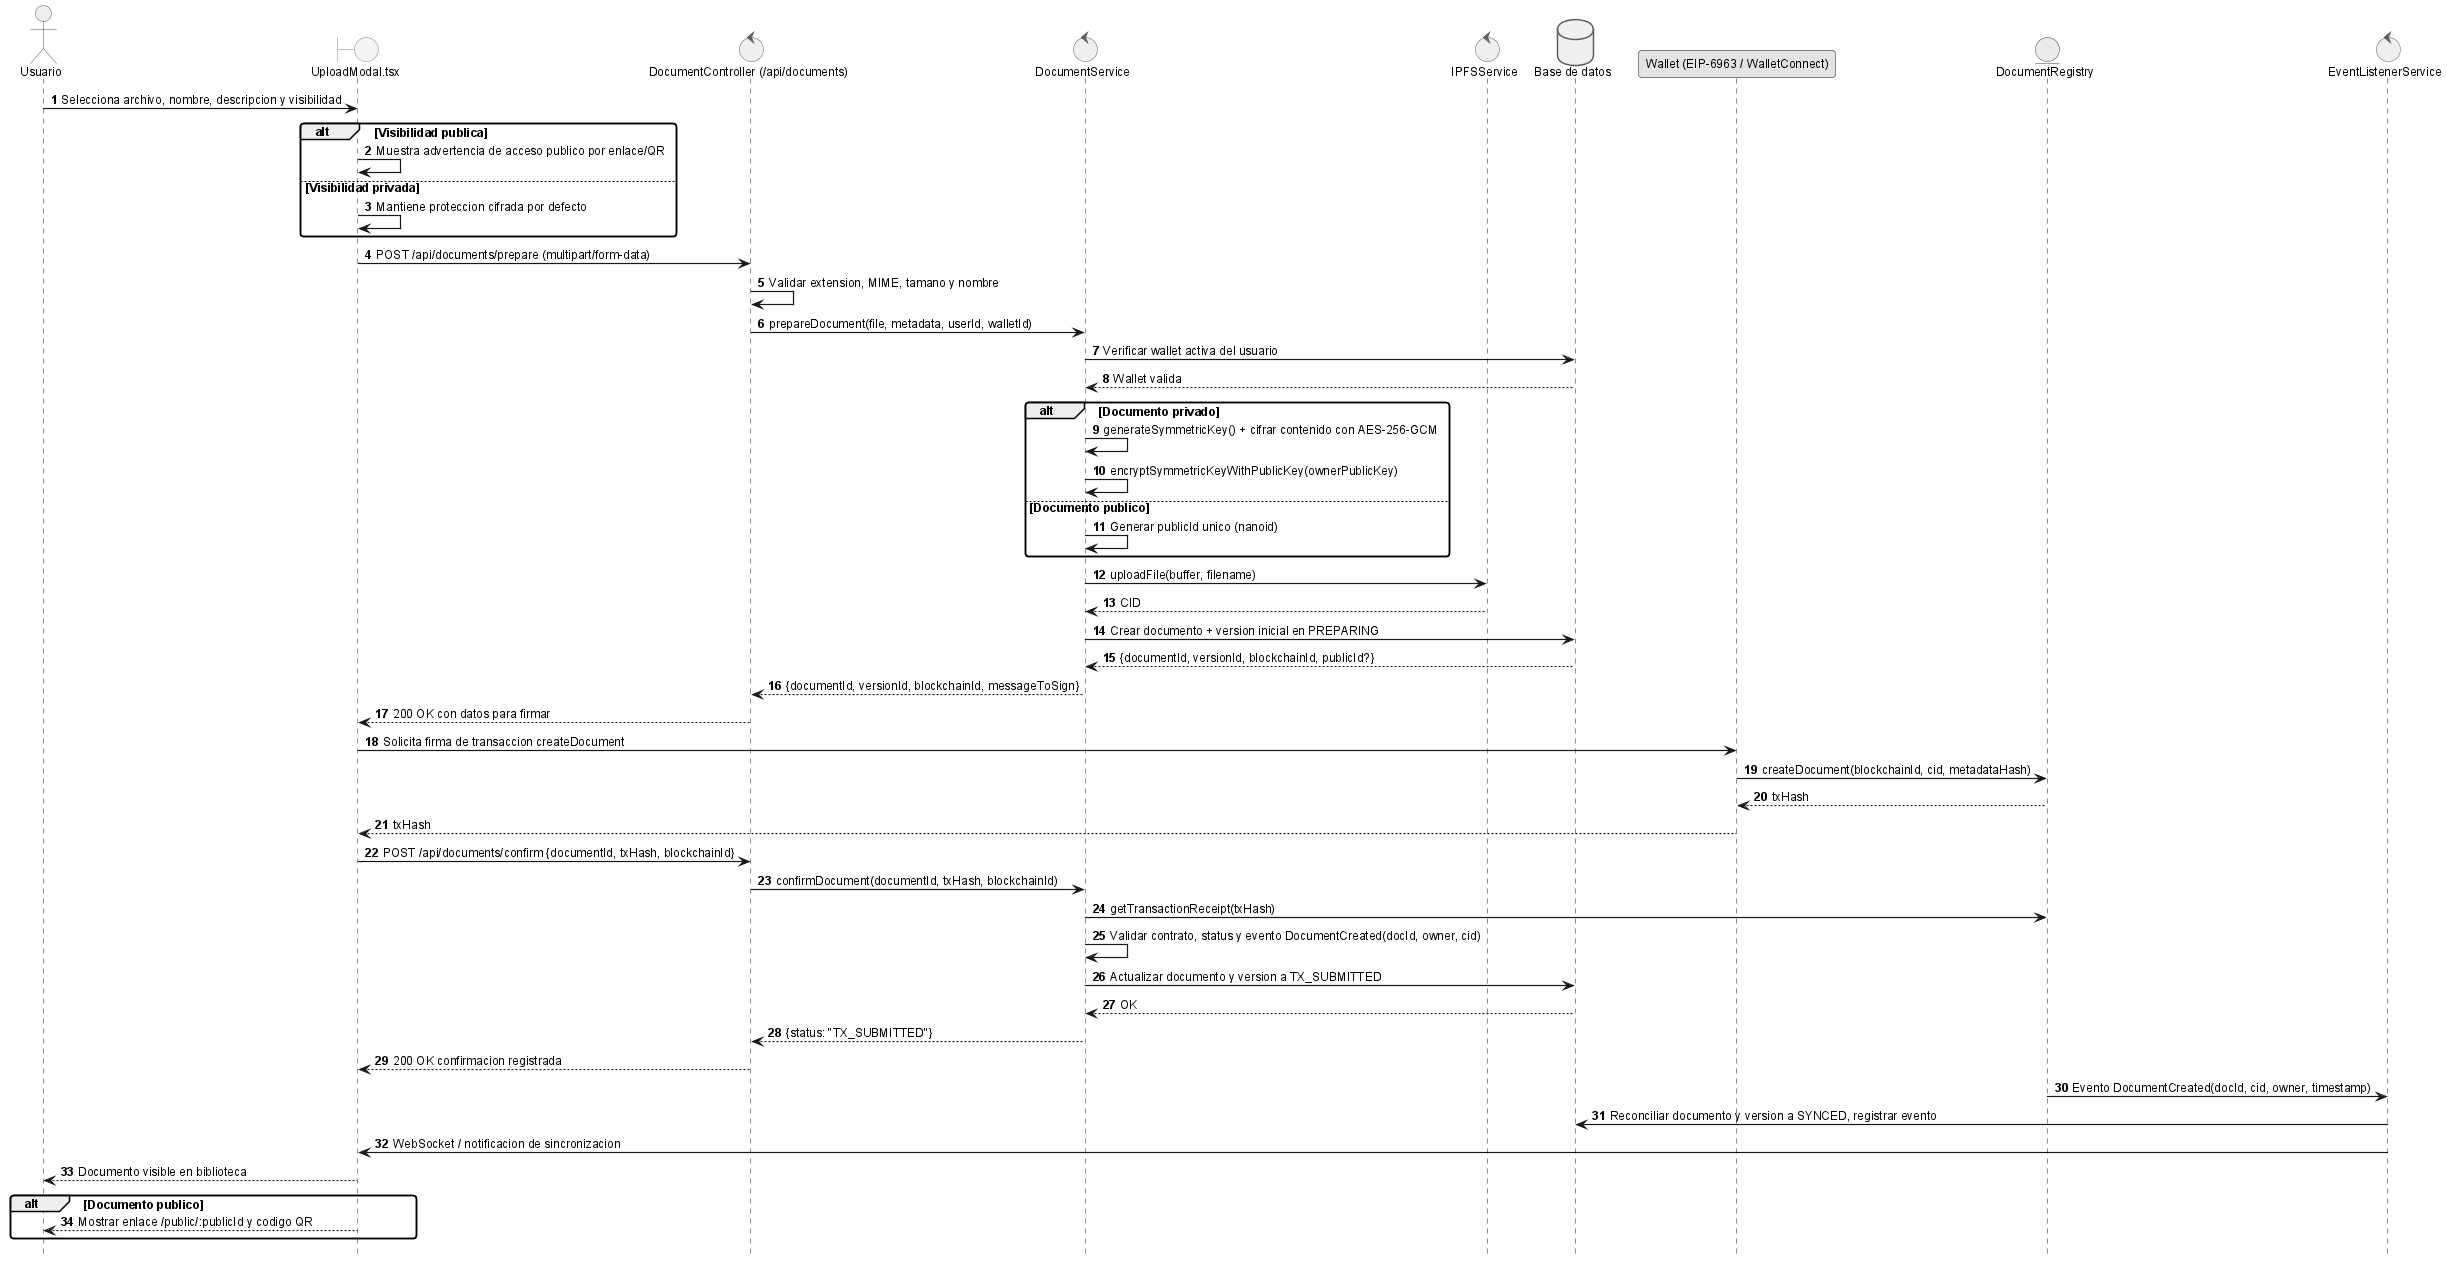
\includegraphics[width=0.9\textwidth]{diagramas/seq-upload.png}\caption{Secuencia de diseño — UC-0015: Subir Documento (flujo completo)}\label{fig:seq-upload}\end{figure}
\begin{figure}[H]\centering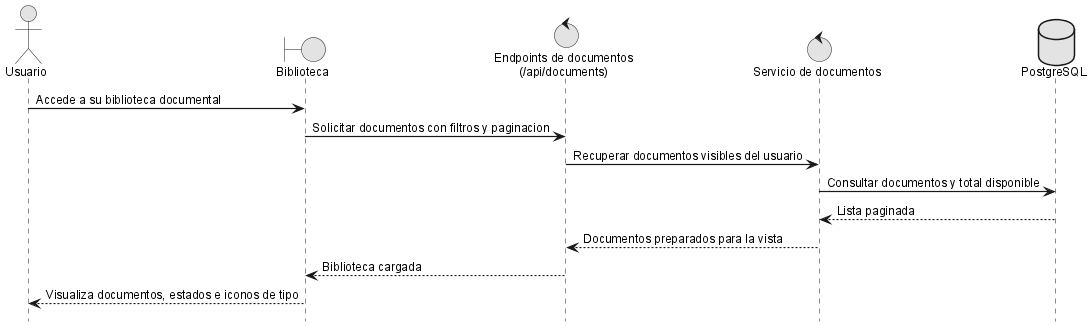
\includegraphics[width=0.9\textwidth]{diagramas/seq-list-documents.png}\caption{Secuencia de diseño — UC-0016: Listar Documentos}\label{fig:seq-list-documents}\end{figure}
\begin{figure}[H]\centering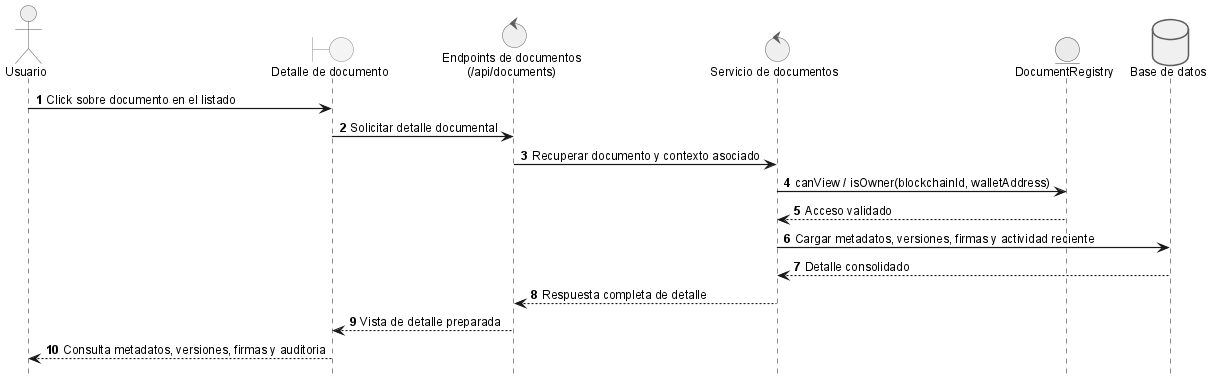
\includegraphics[width=0.9\textwidth]{diagramas/seq-doc-detail.png}\caption{Secuencia de diseño — UC-0017: Ver Detalle}\label{fig:seq-doc-detail}\end{figure}
\begin{figure}[H]\centering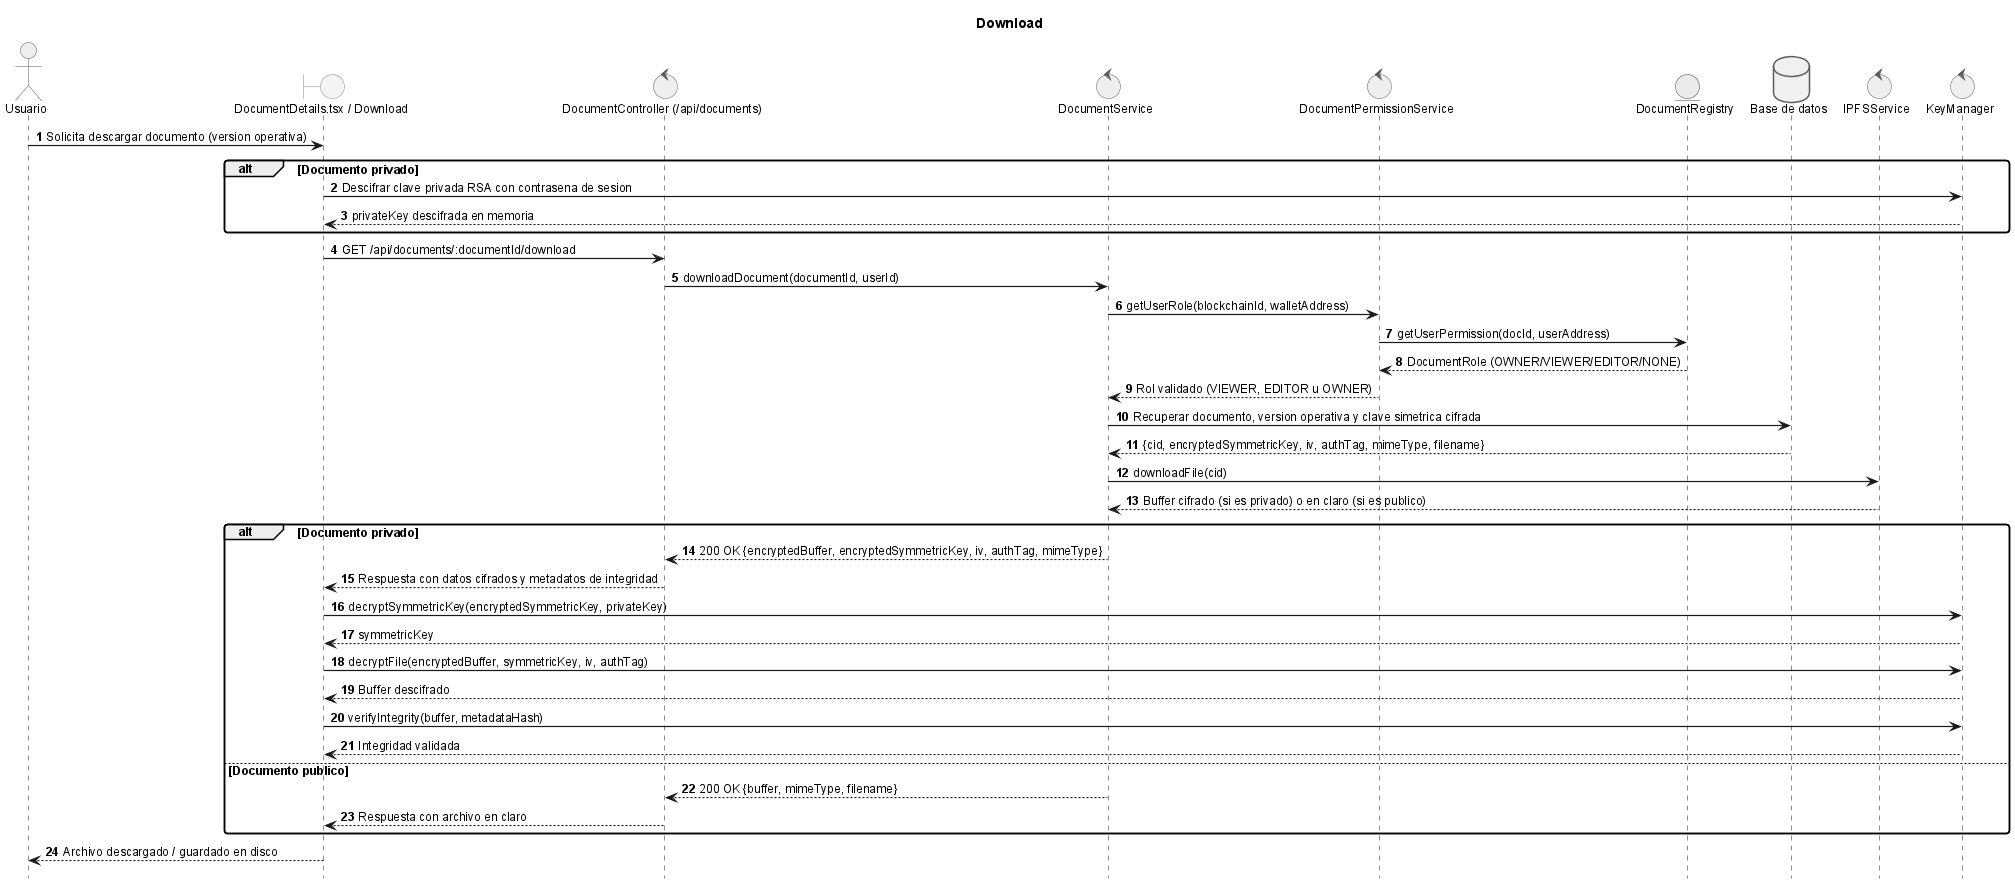
\includegraphics[width=0.9\textwidth]{diagramas/seq-download.png}\caption{Secuencia de diseño — UC-0018: Descargar Documento}\label{fig:seq-download}\end{figure}
\begin{figure}[H]\centering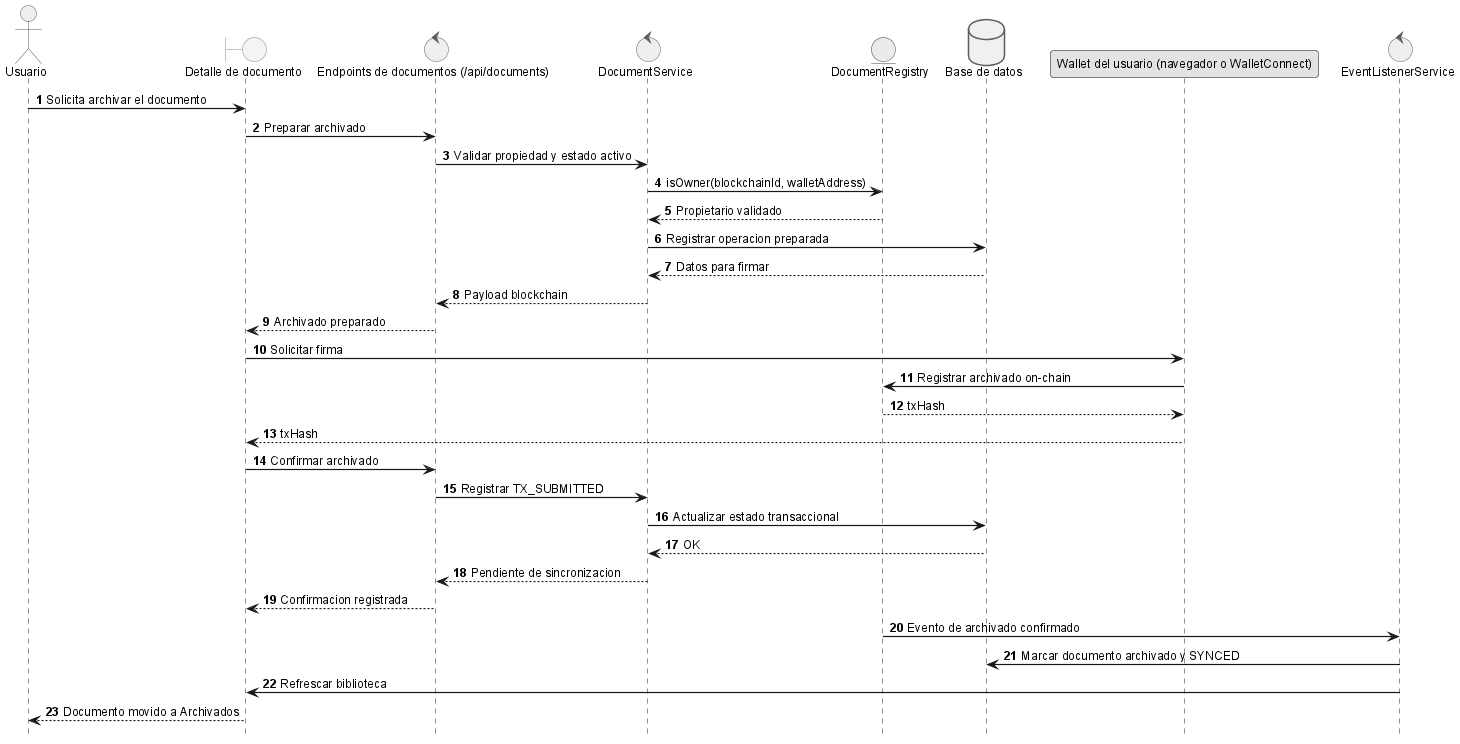
\includegraphics[width=0.9\textwidth]{diagramas/seq-archive.png}\caption{Secuencia de diseño — UC-0019: Archivar Documento}\label{fig:seq-archive}\end{figure}
\begin{figure}[H]\centering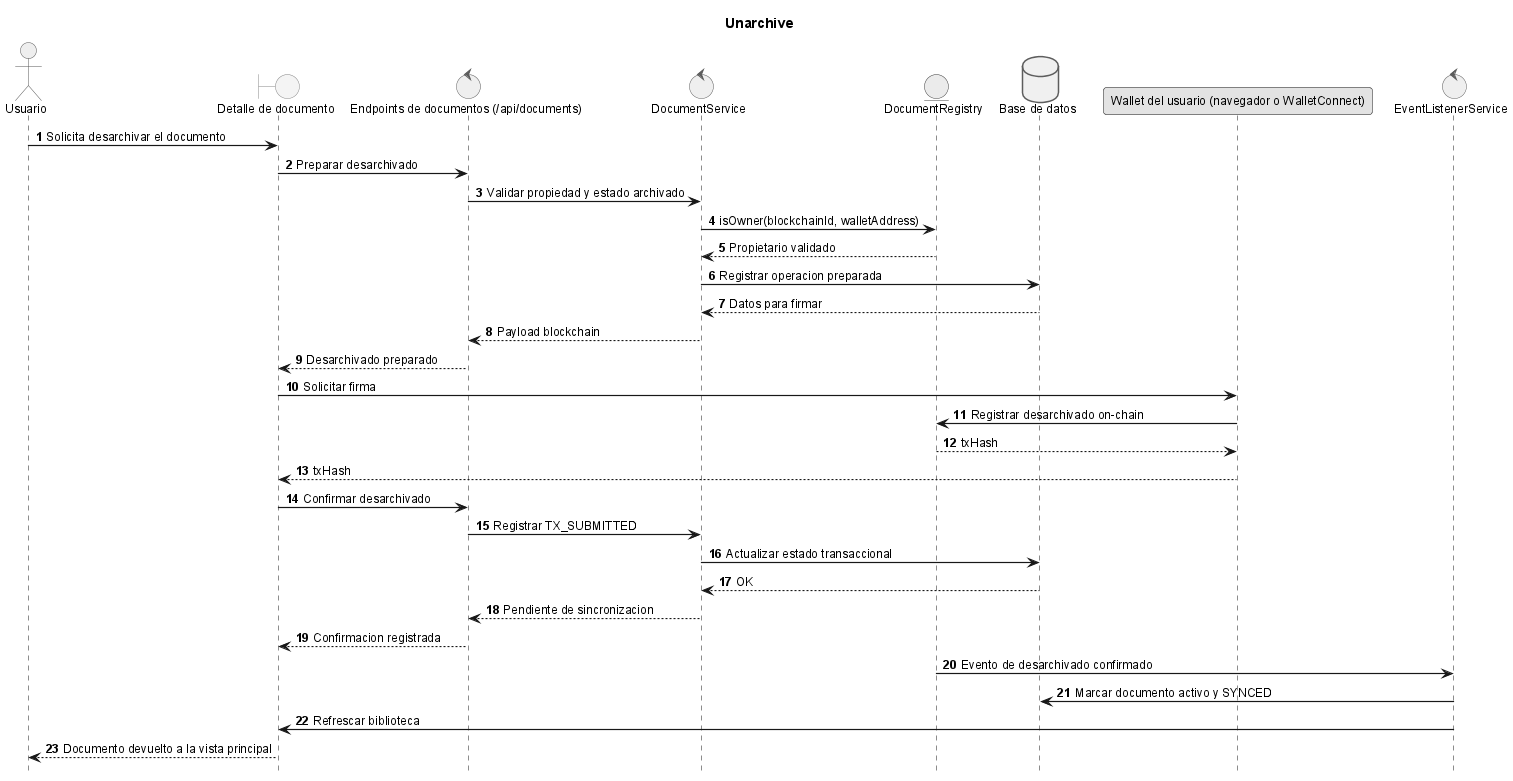
\includegraphics[width=0.9\textwidth]{diagramas/seq-unarchive.png}\caption{Secuencia de diseño — UC-0020: Desarchivar Documento}\label{fig:seq-unarchive}\end{figure}
\begin{figure}[H]\centering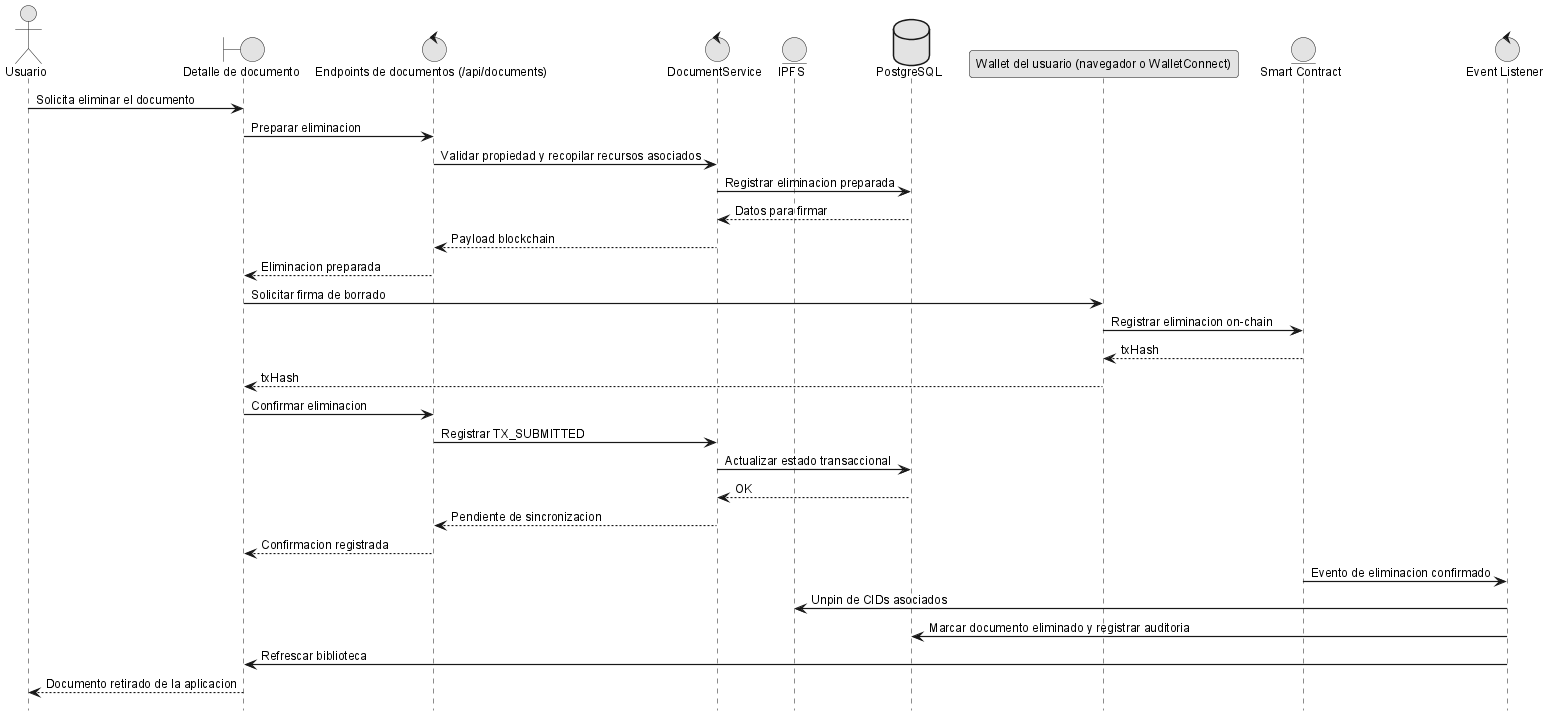
\includegraphics[width=0.9\textwidth]{diagramas/seq-delete.png}\caption{Secuencia de diseño — UC-0021: Eliminar Documento}\label{fig:seq-delete}\end{figure}
\begin{figure}[H]\centering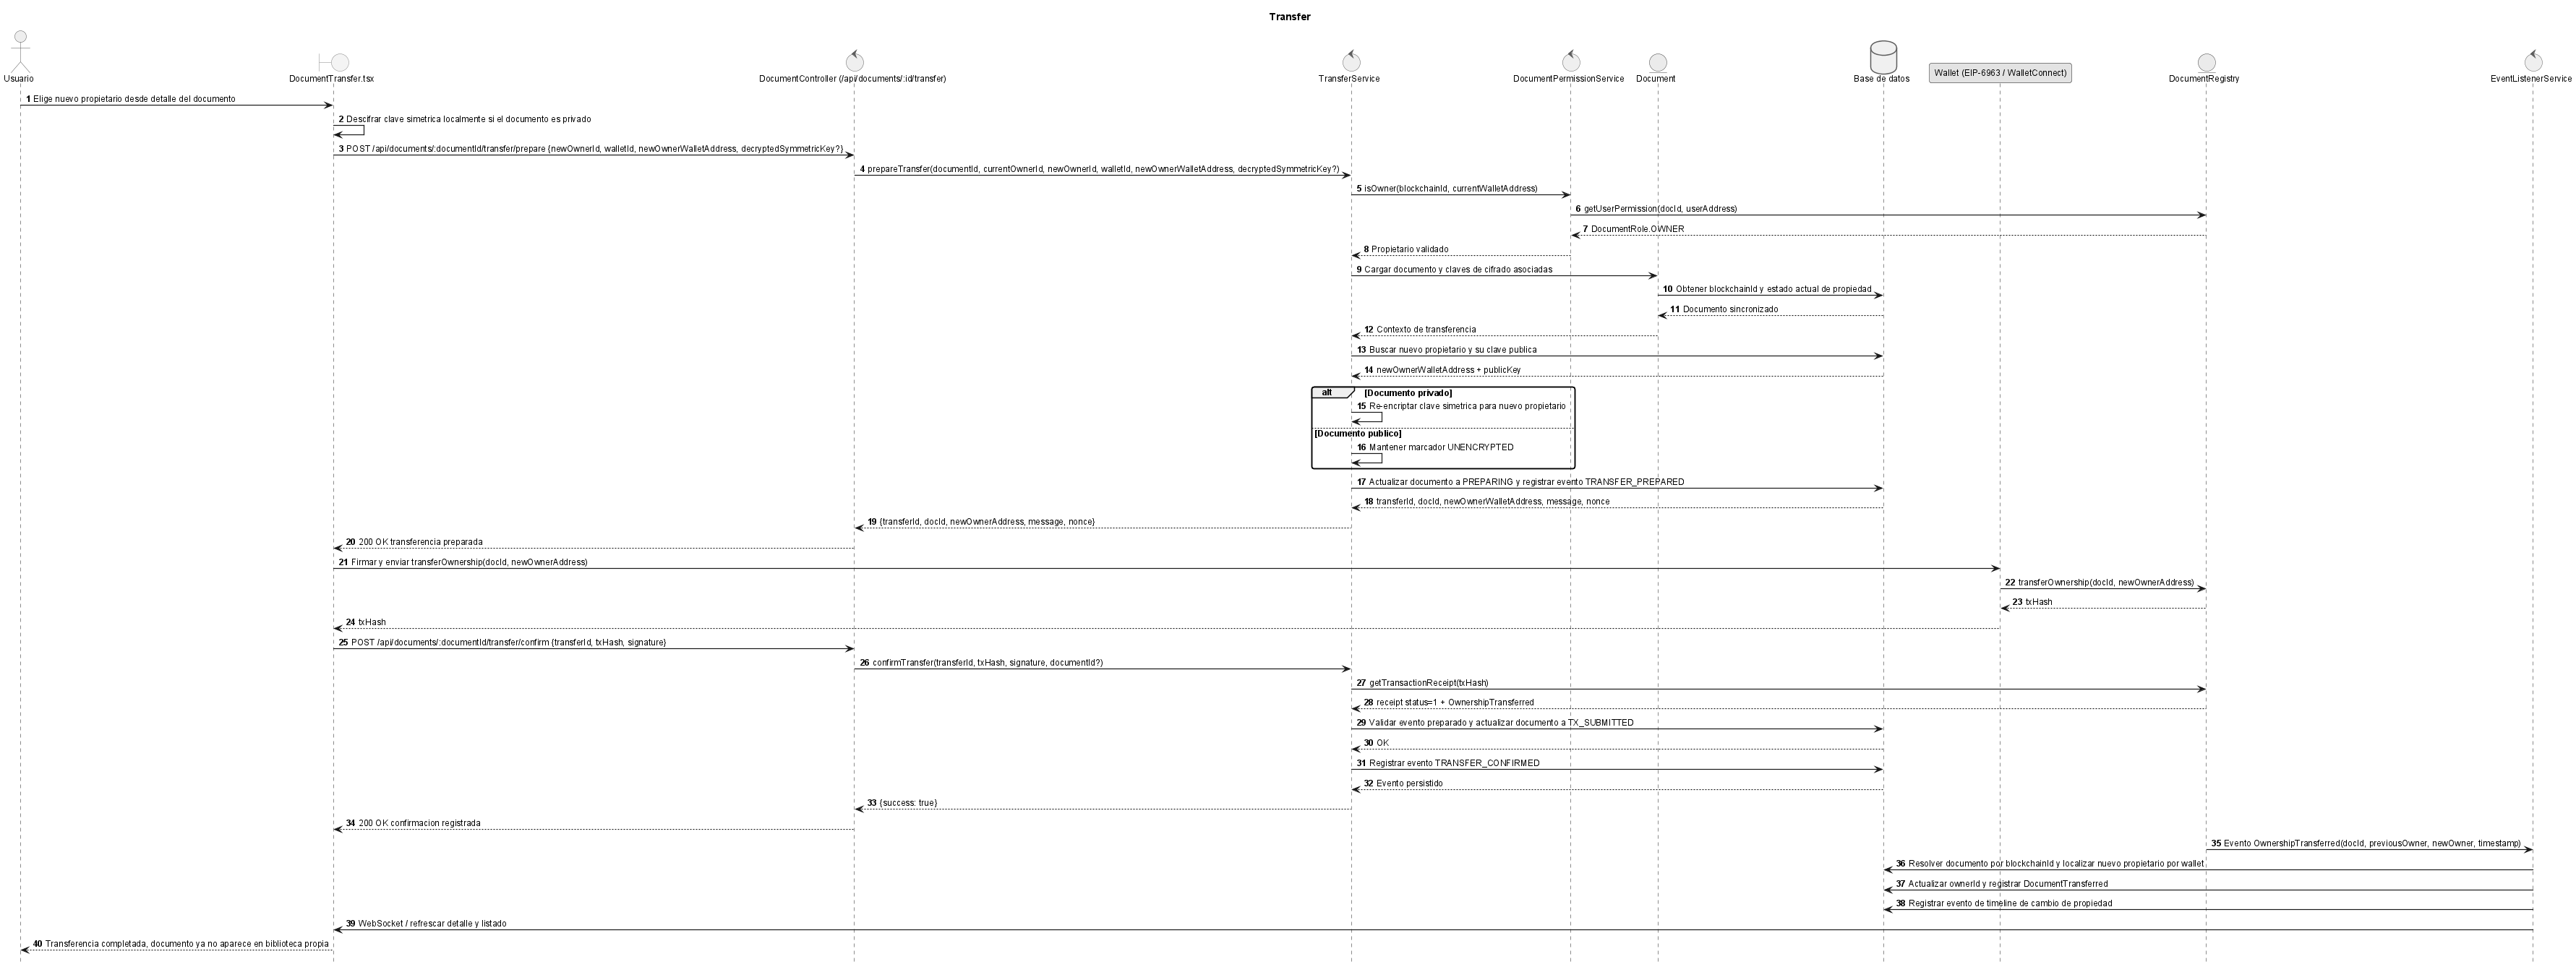
\includegraphics[width=0.9\textwidth]{diagramas/seq-transfer.png}\caption{Secuencia de diseño — UC-0022: Transferir Documento}\label{fig:seq-transfer}\end{figure}
\begin{figure}[H]\centering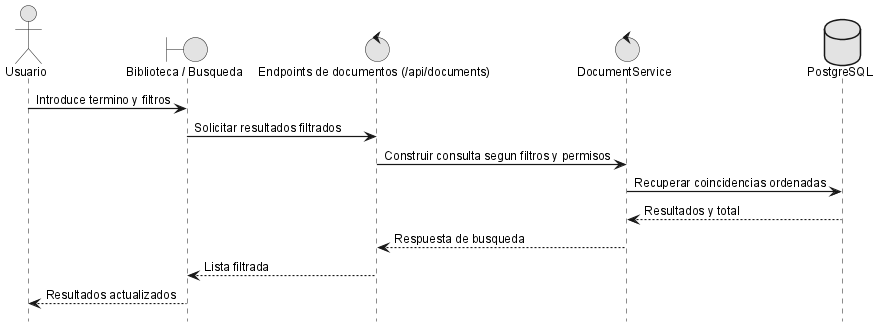
\includegraphics[width=0.9\textwidth]{diagramas/seq-search.png}\caption{Secuencia de diseño — UC-0023: Buscar Documentos}\label{fig:seq-search}\end{figure}
\begin{figure}[H]\centering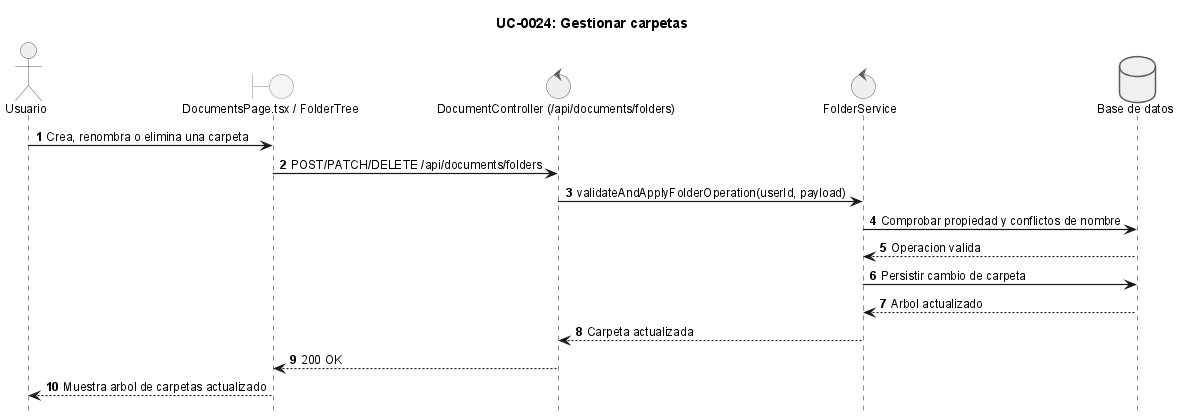
\includegraphics[width=0.9\textwidth]{diagramas/seq-manage-folders.png}\caption{Secuencia de diseño — UC-0024: Gestionar Carpetas}\label{fig:seq-manage-folders}\end{figure}
\begin{figure}[H]\centering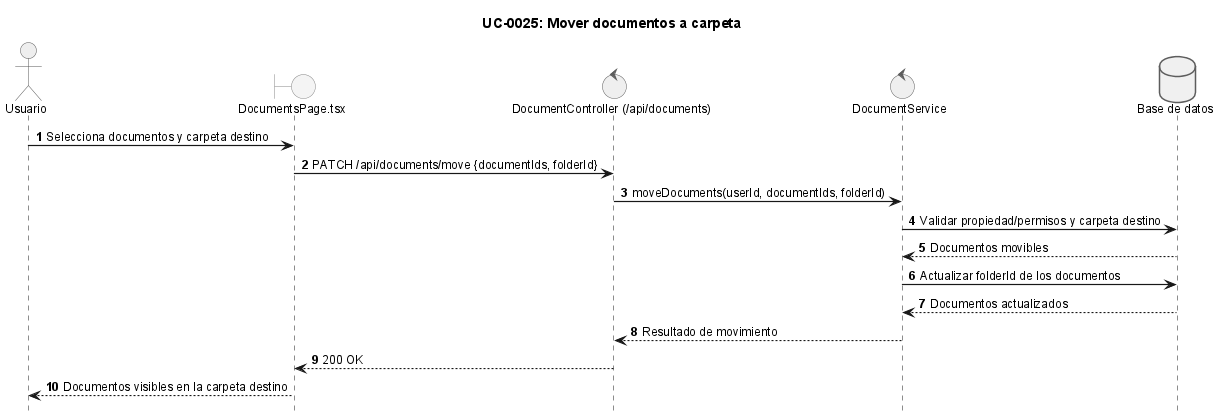
\includegraphics[width=0.9\textwidth]{diagramas/seq-move-documents.png}\caption{Secuencia de diseño — UC-0025: Mover Documentos}\label{fig:seq-move-documents}\end{figure}

\subsection{Versiones}

\begin{figure}[H]\centering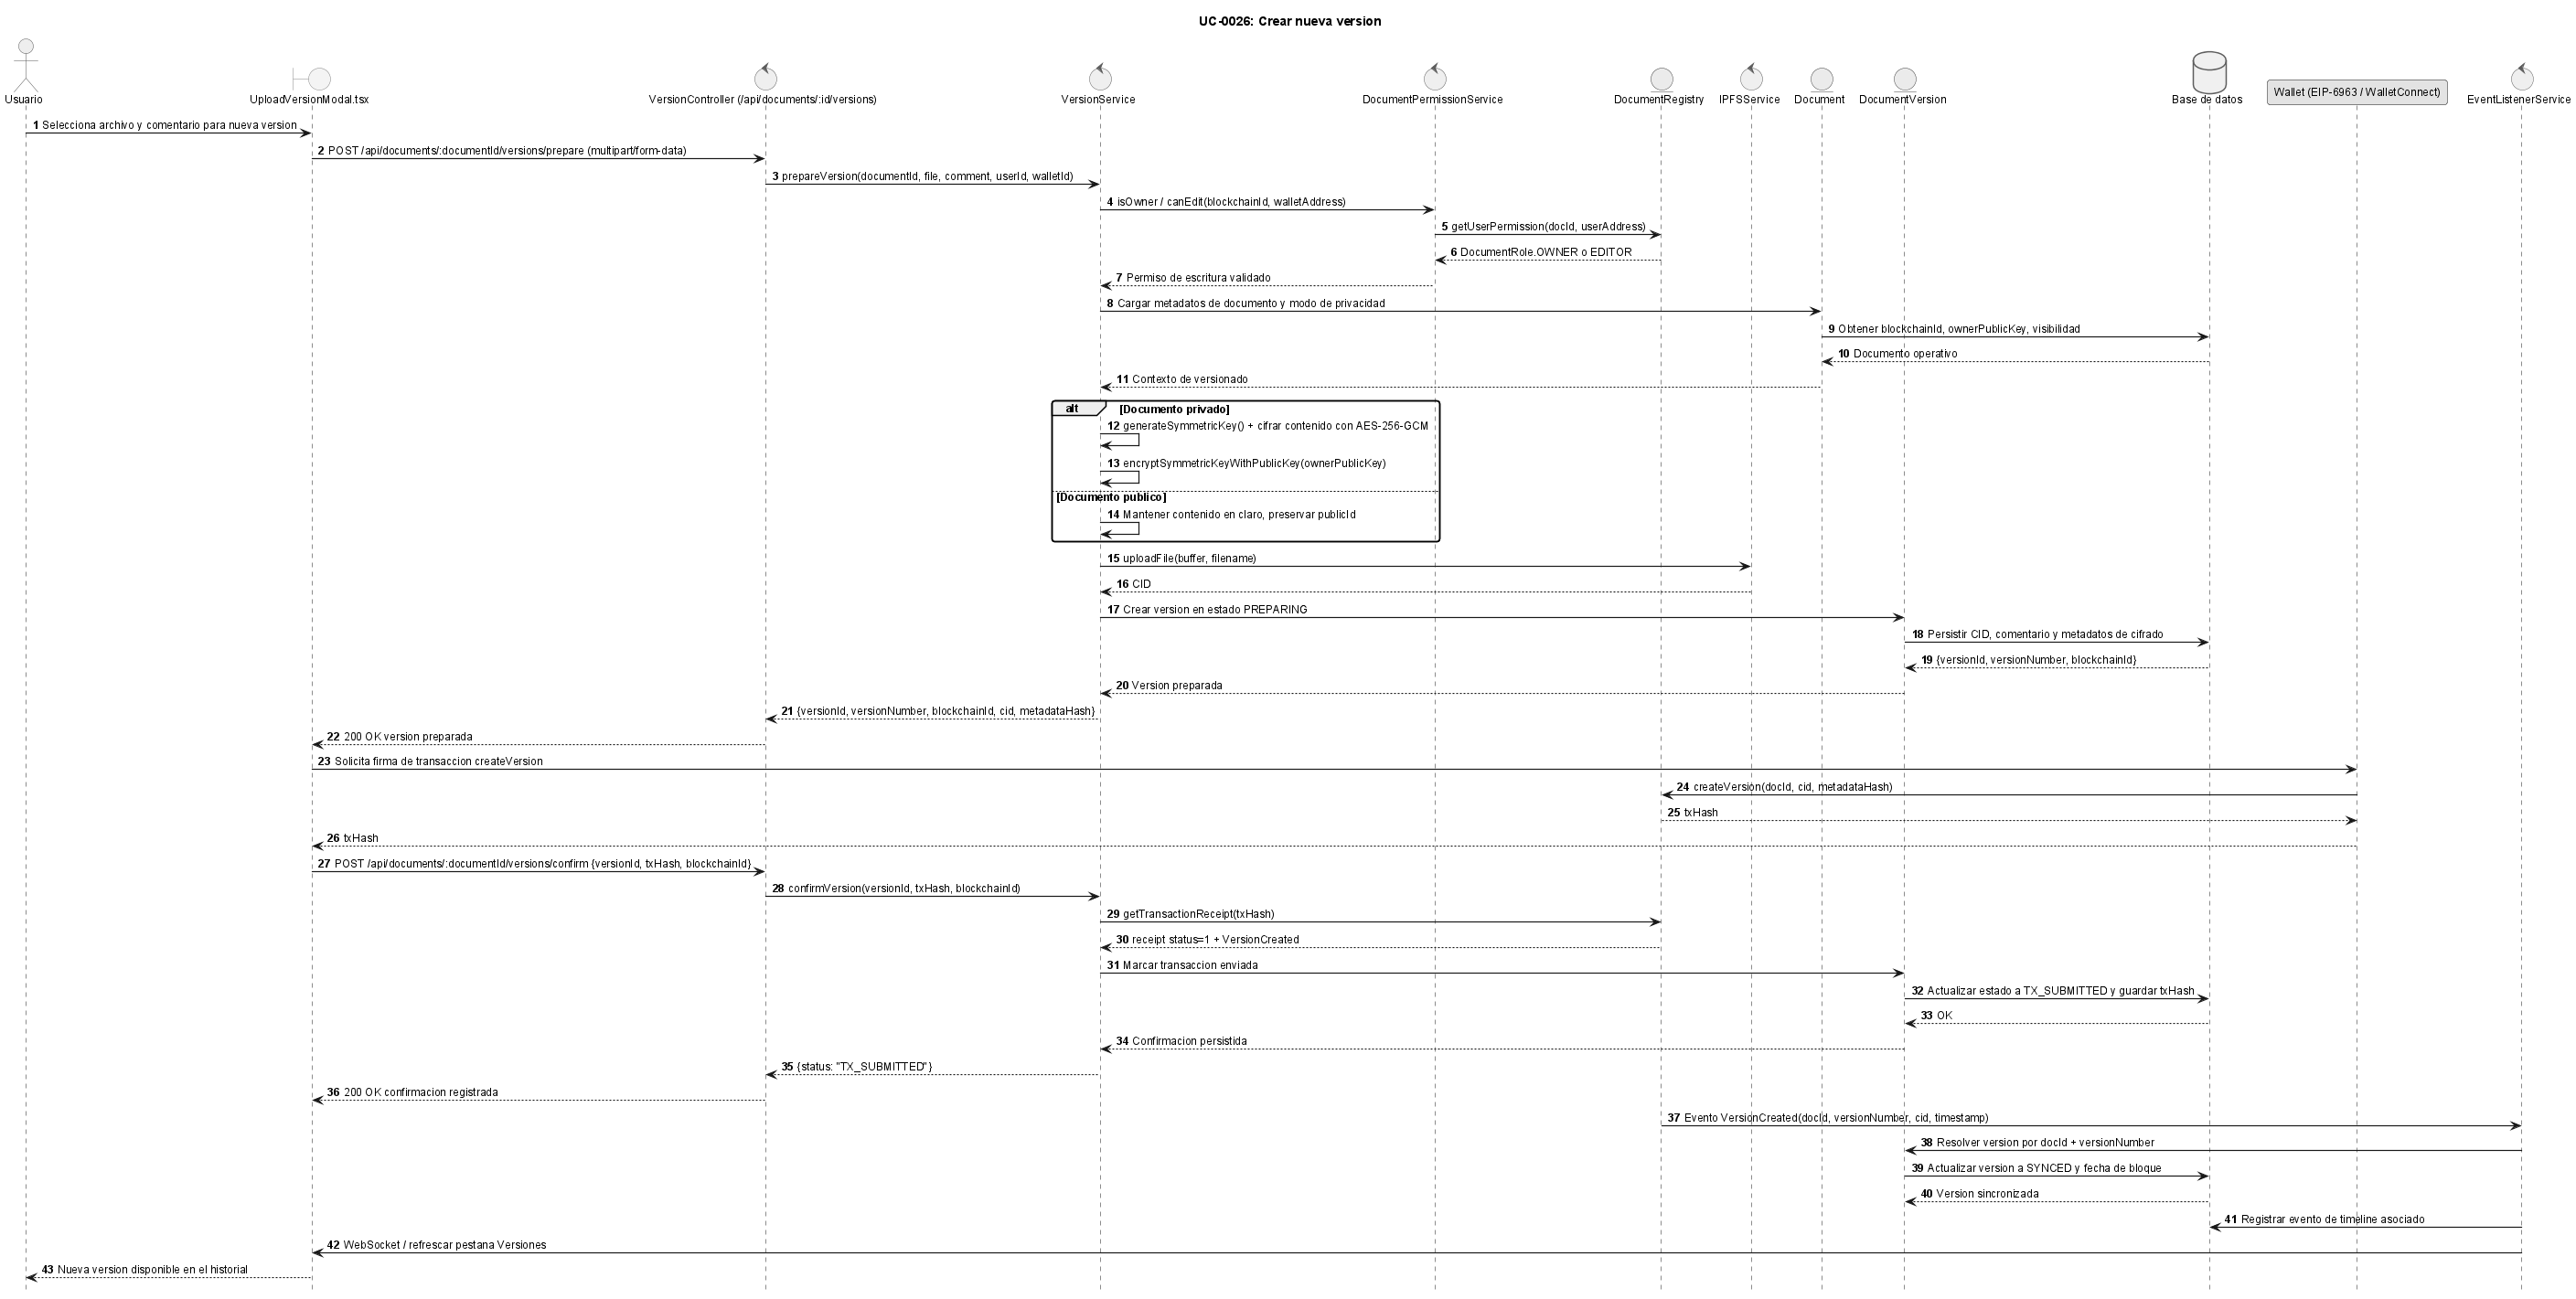
\includegraphics[width=0.9\textwidth]{diagramas/seq-version.png}\caption{Secuencia de diseño — UC-0026: Crear Nueva Versión}\label{fig:seq-version}\end{figure}
\begin{figure}[H]\centering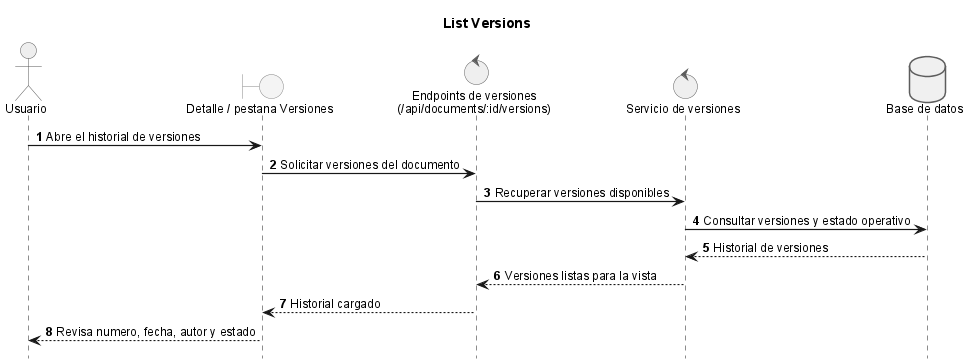
\includegraphics[width=0.9\textwidth]{diagramas/seq-list-versions.png}\caption{Secuencia de diseño — UC-0027: Listar Versiones}\label{fig:seq-list-versions}\end{figure}
\begin{figure}[H]\centering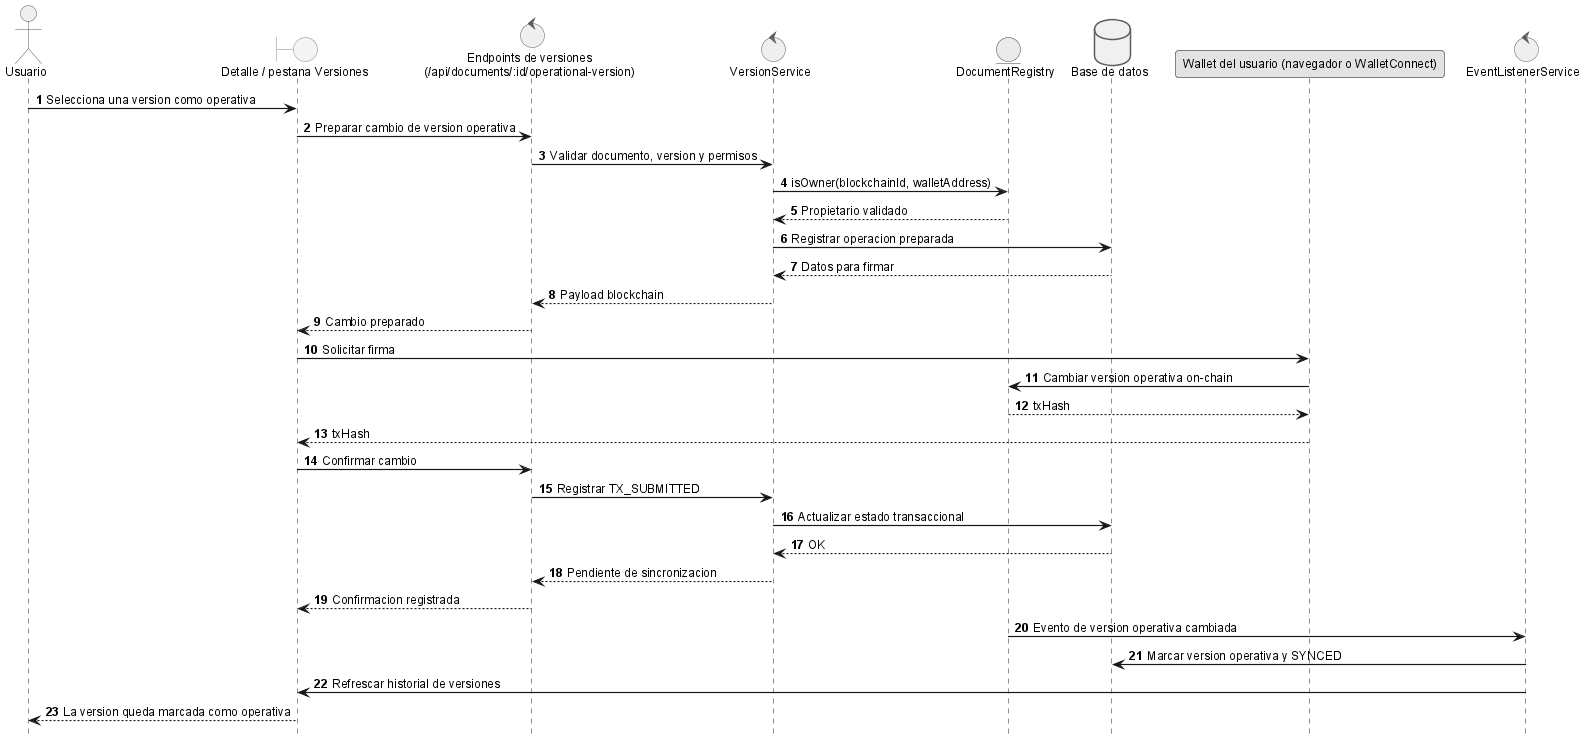
\includegraphics[width=0.9\textwidth]{diagramas/seq-activate-version.png}\caption{Secuencia de diseño — UC-0028: Versión Operativa}\label{fig:seq-activate-version}\end{figure}
\begin{figure}[H]\centering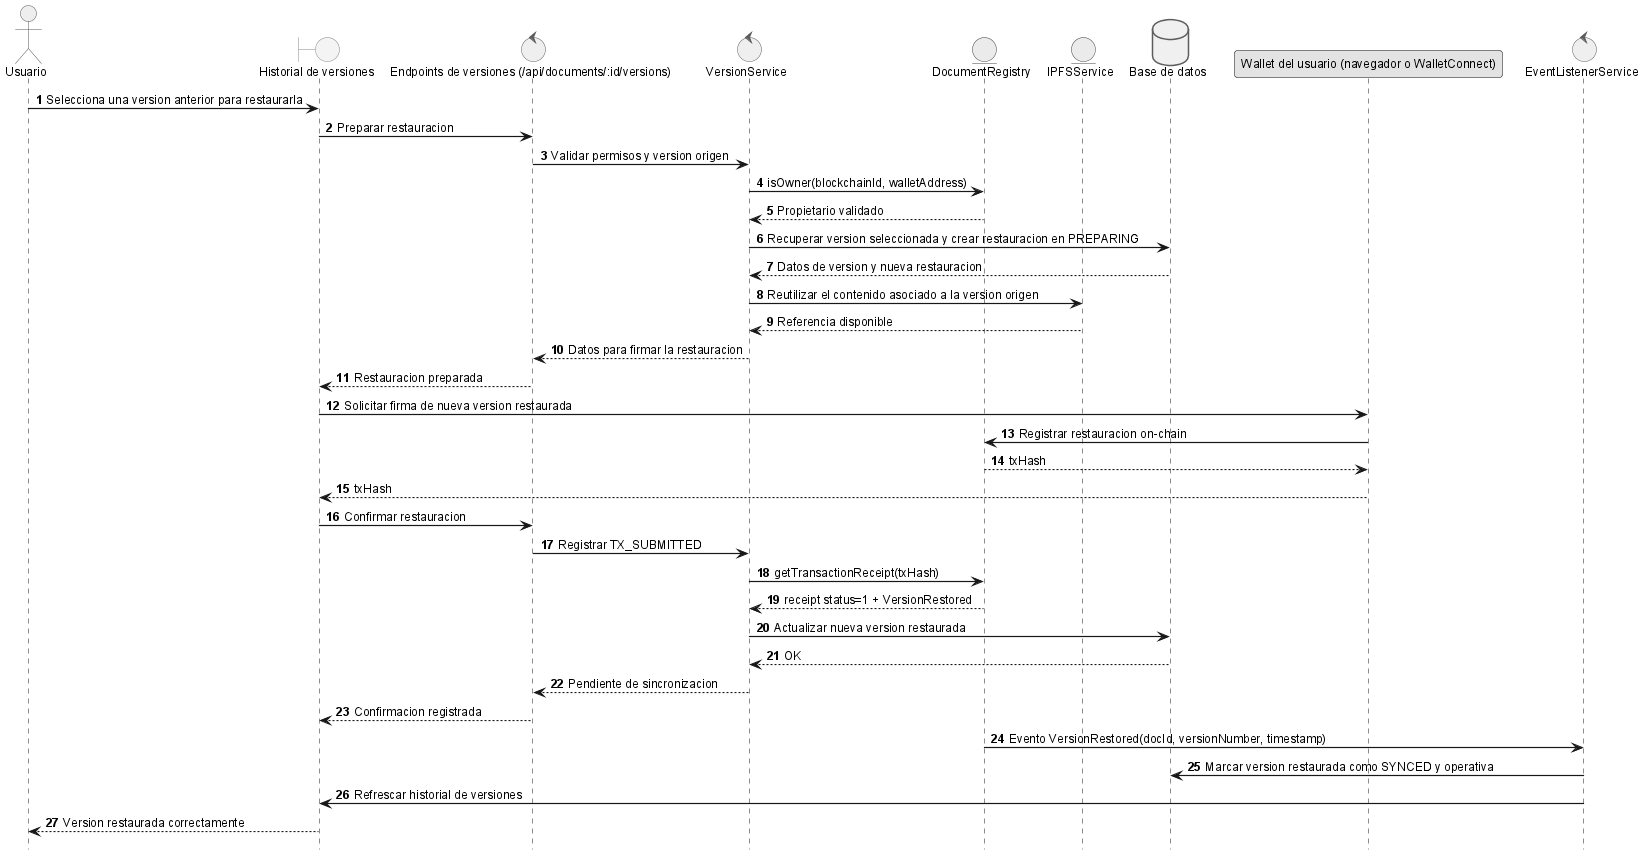
\includegraphics[width=0.9\textwidth]{diagramas/seq-restore-version.png}\caption{Secuencia de diseño — UC-0029: Restaurar Versión}\label{fig:seq-restore-version}\end{figure}
\begin{figure}[H]\centering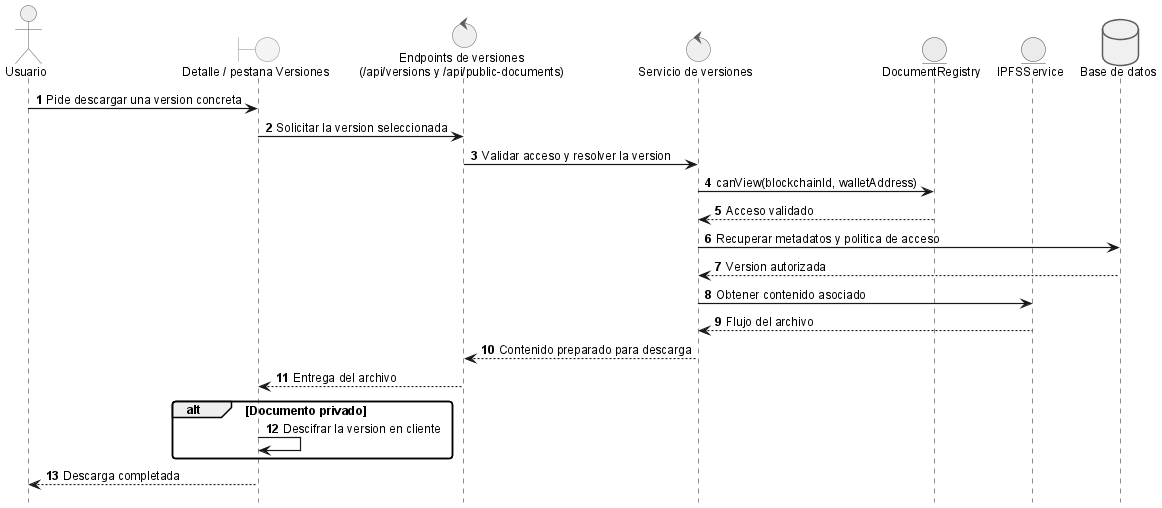
\includegraphics[width=0.9\textwidth]{diagramas/seq-download-version.png}\caption{Secuencia de diseño — UC-0030: Descargar Versión}\label{fig:seq-download-version}\end{figure}

\subsection{Firmas digitales}

\begin{figure}[H]\centering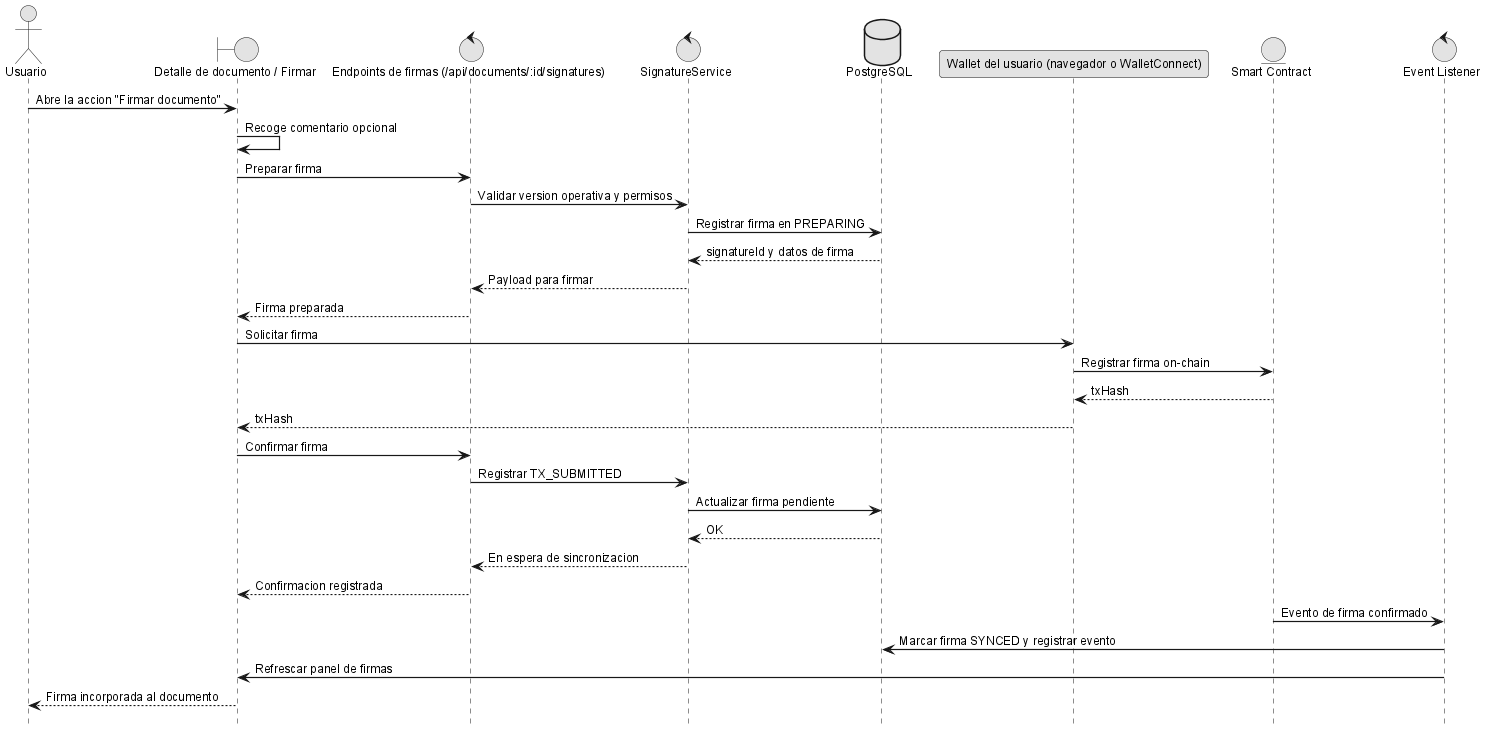
\includegraphics[width=0.9\textwidth]{diagramas/seq-sign.png}\caption{Secuencia de diseño — UC-0031: Firmar Documento}\label{fig:seq-sign}\end{figure}
\begin{figure}[H]\centering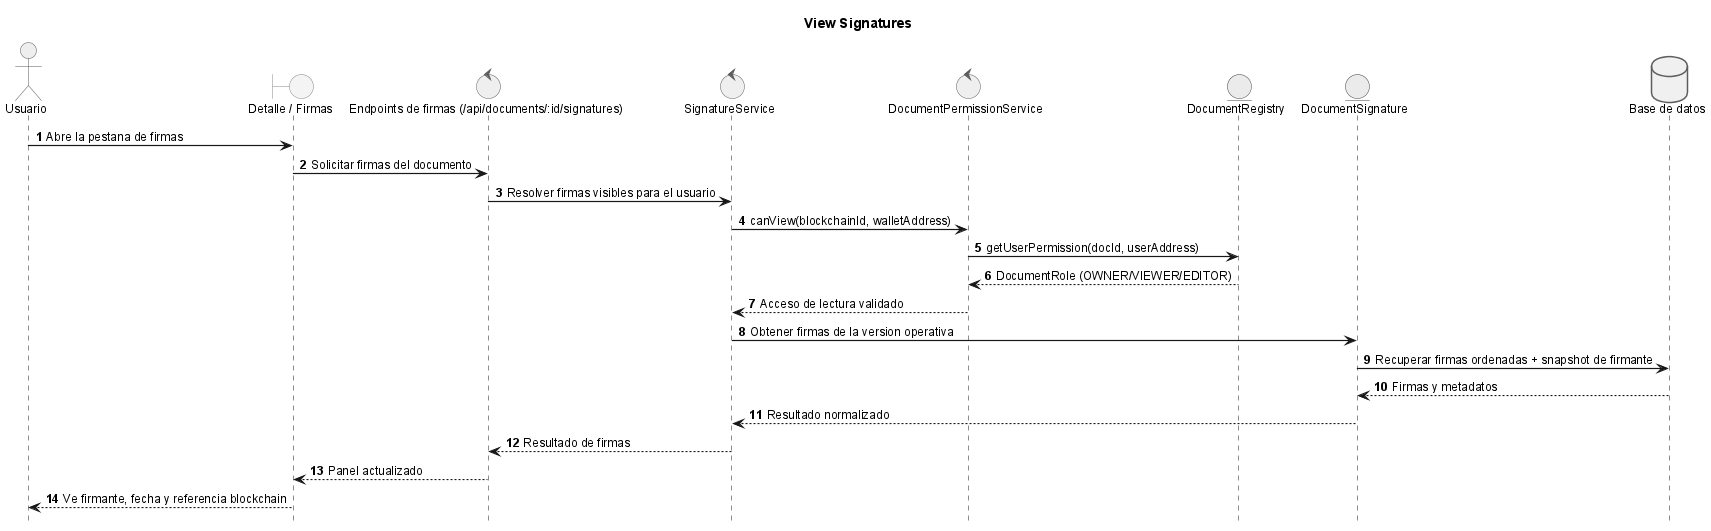
\includegraphics[width=0.9\textwidth]{diagramas/seq-view-signatures.png}\caption{Secuencia de diseño — UC-0032: Ver Firmas}\label{fig:seq-view-signatures}\end{figure}
\begin{figure}[H]\centering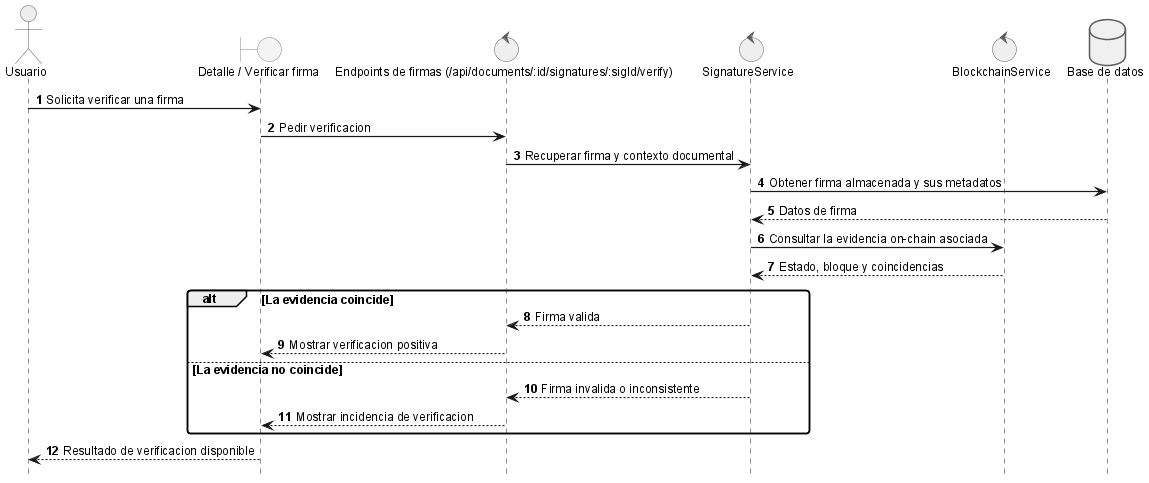
\includegraphics[width=0.9\textwidth]{diagramas/seq-verify-signature.png}\caption{Secuencia de diseño — UC-0033: Verificar Firma}\label{fig:seq-verify-signature}\end{figure}

\subsection{Compartición}

\begin{figure}[H]\centering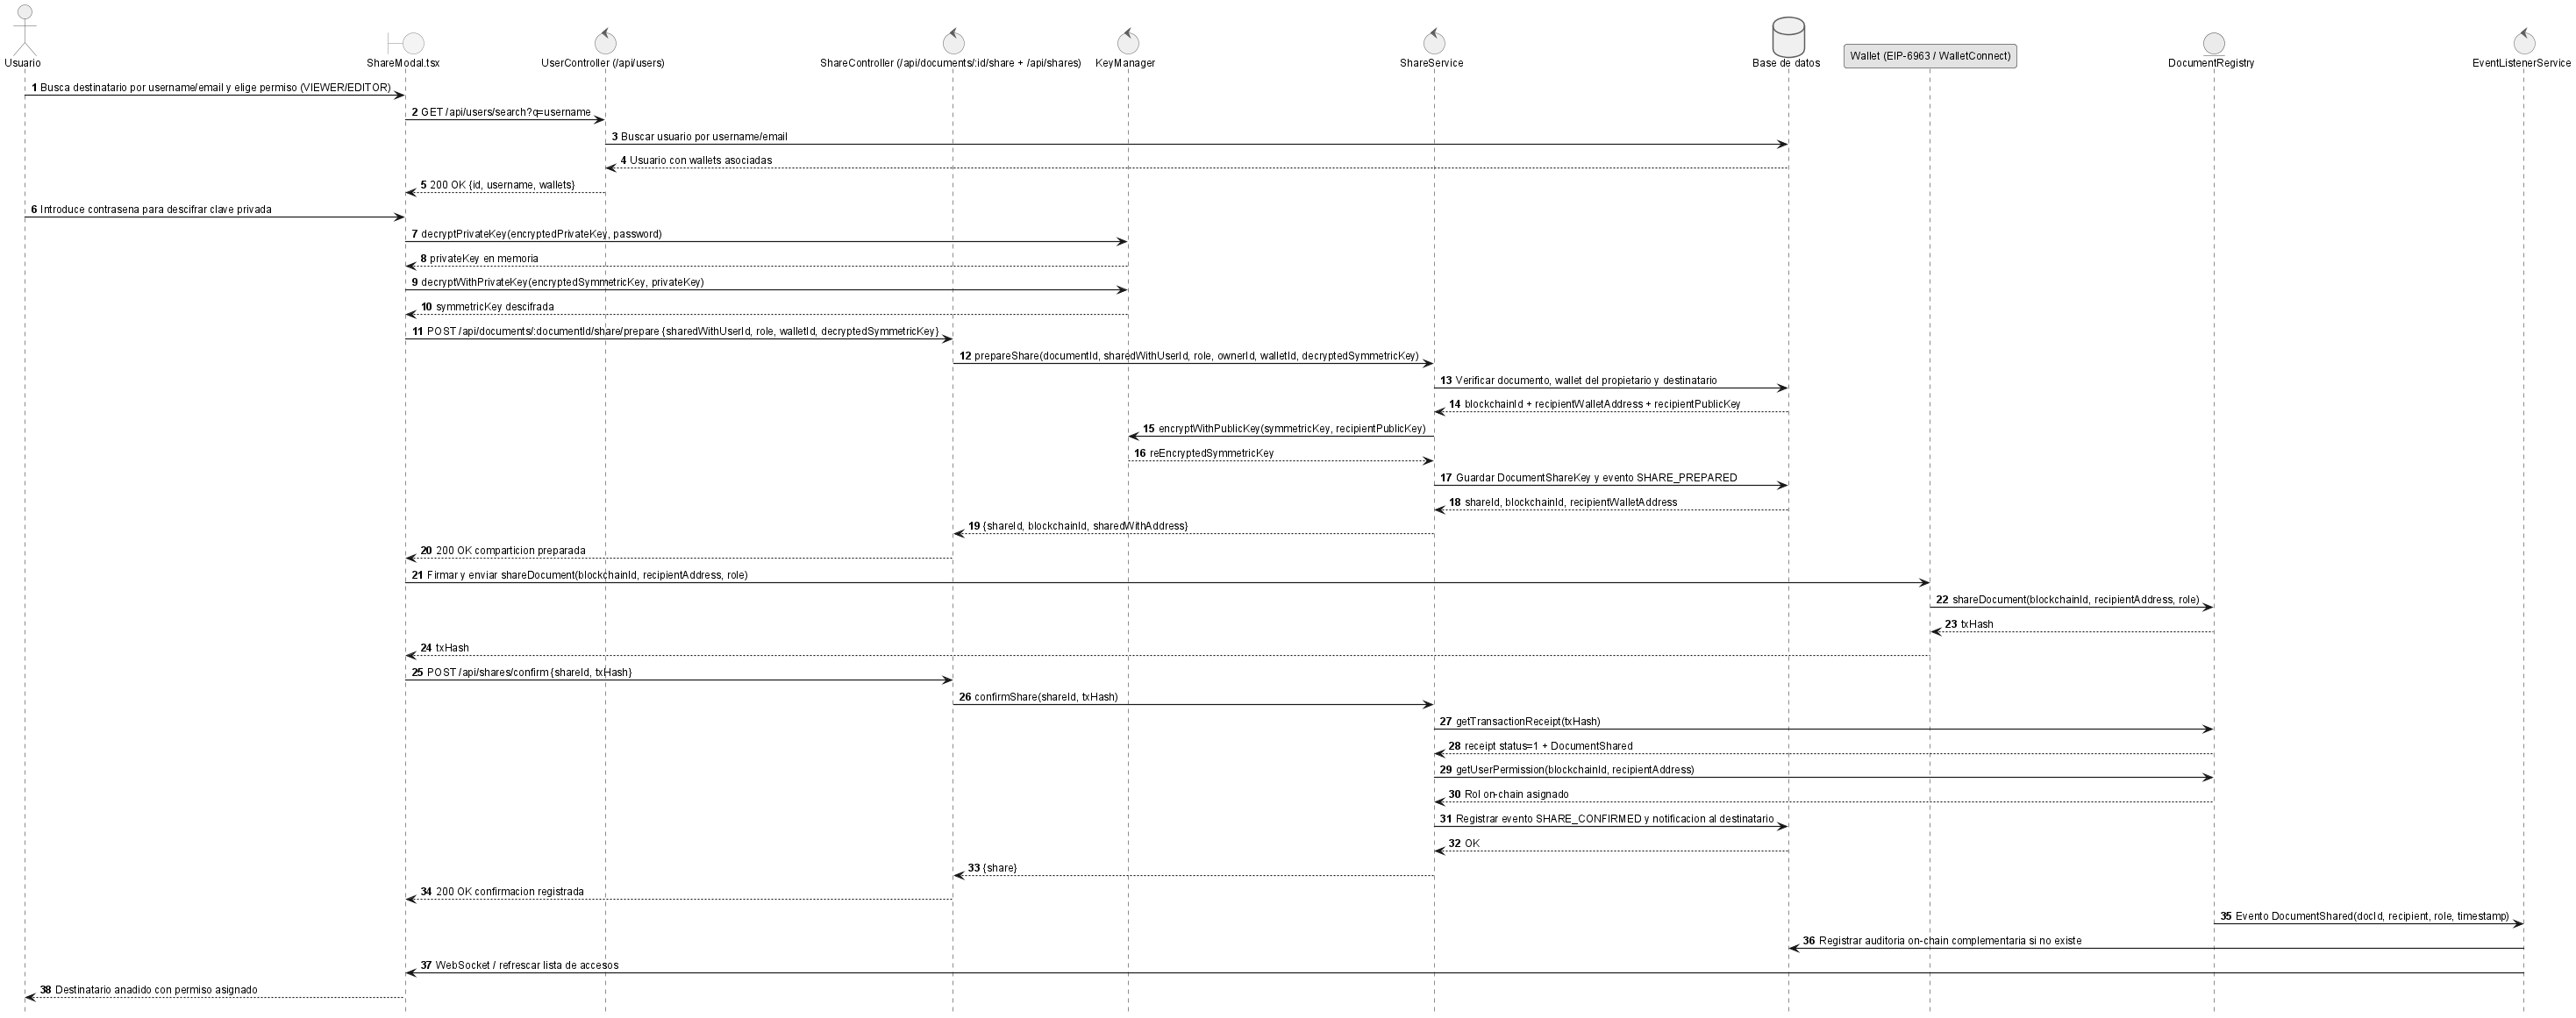
\includegraphics[width=0.9\textwidth]{diagramas/seq-share.png}\caption{Secuencia de diseño — UC-0034: Compartir Documento}\label{fig:seq-share}\end{figure}
\begin{figure}[H]\centering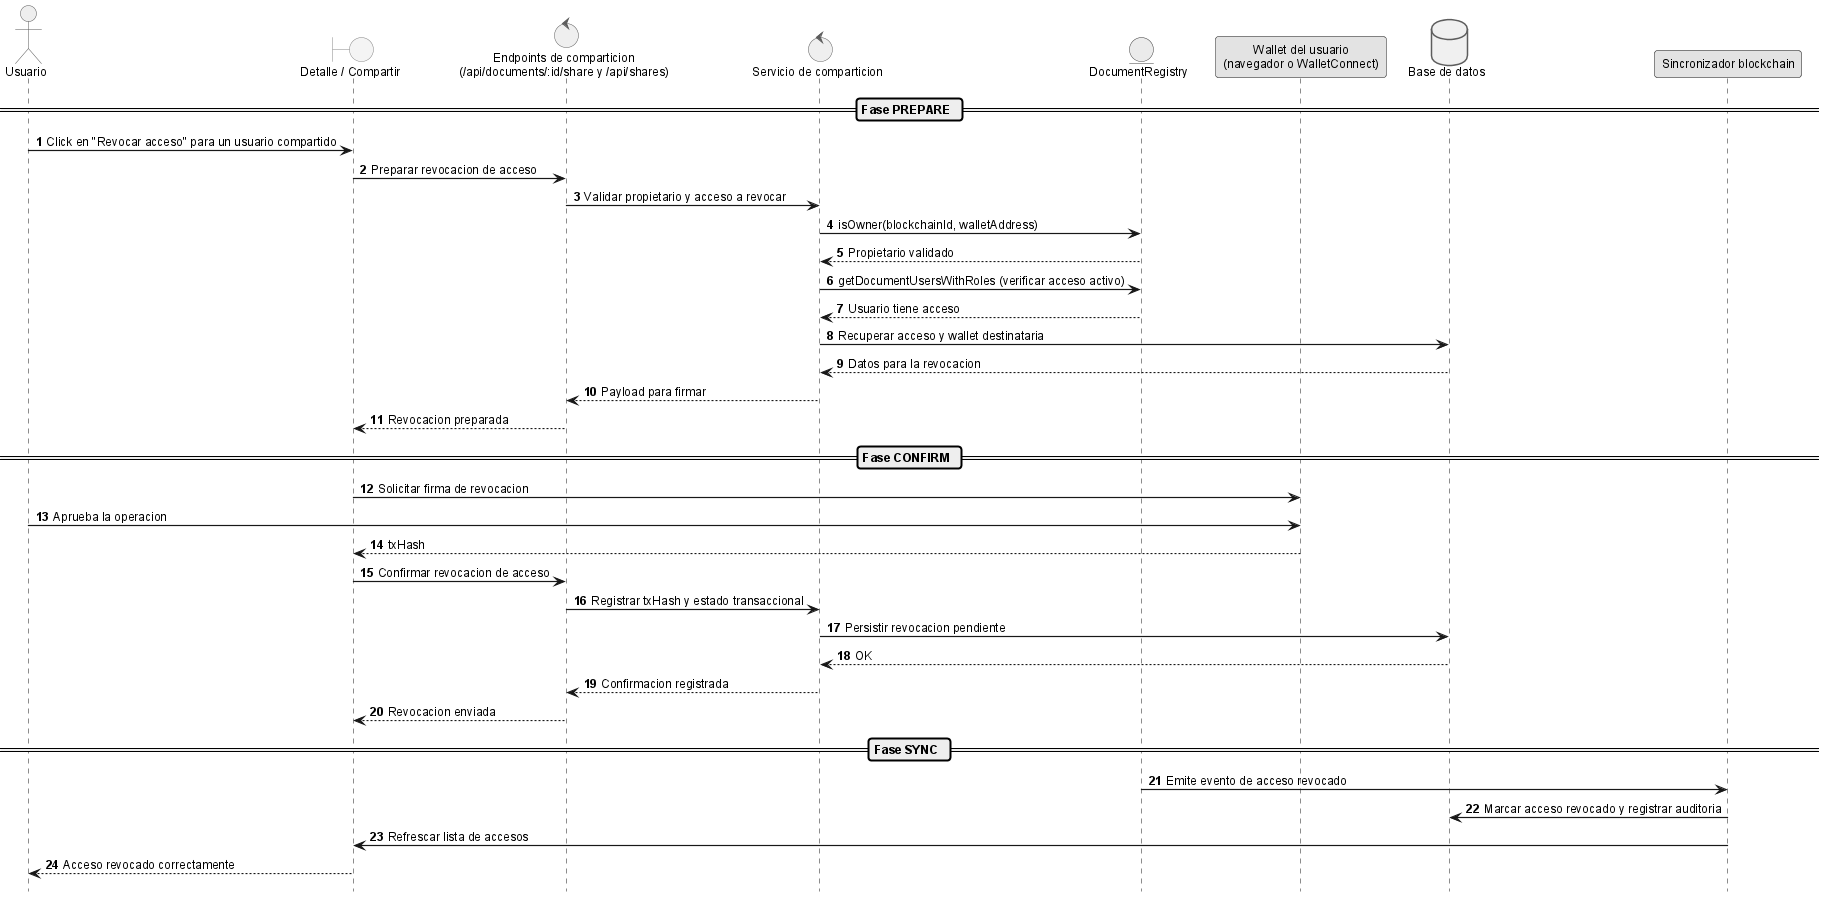
\includegraphics[width=0.9\textwidth]{diagramas/seq-revoke-access.png}\caption{Secuencia de diseño — UC-0035: Revocar Acceso}\label{fig:seq-revoke-access}\end{figure}
\begin{figure}[H]\centering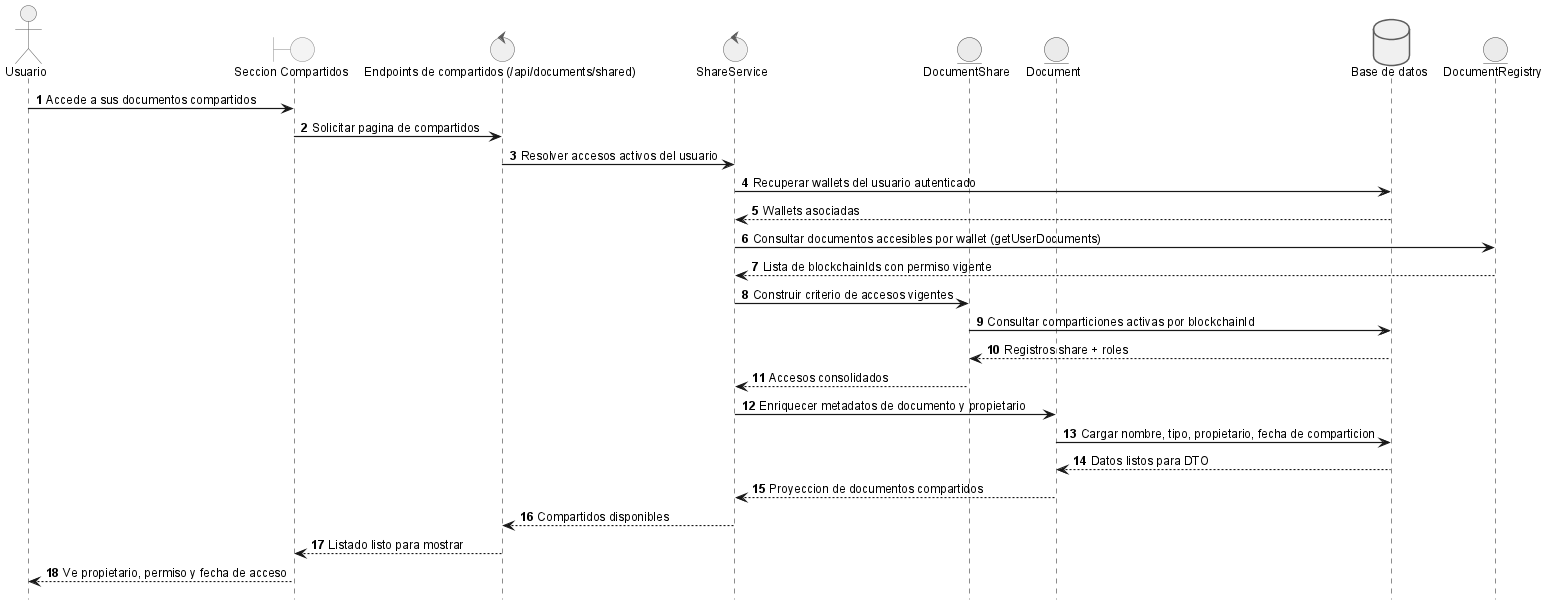
\includegraphics[width=0.9\textwidth]{diagramas/seq-shared-documents.png}\caption{Secuencia de diseño — UC-0036: Compartidos Conmigo}\label{fig:seq-shared-documents}\end{figure}

\subsection{Auditoría, verificación y administración}

\begin{figure}[H]\centering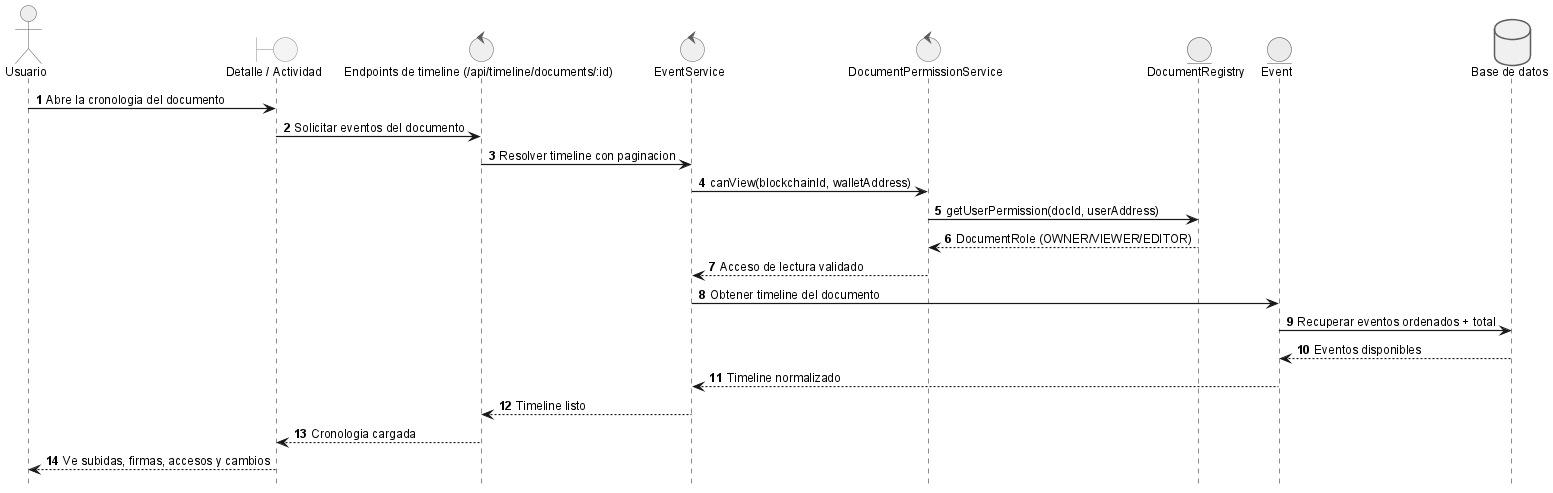
\includegraphics[width=0.9\textwidth]{diagramas/seq-timeline.png}\caption{Secuencia de diseño — UC-0037: Timeline}\label{fig:seq-timeline}\end{figure}
\begin{figure}[H]\centering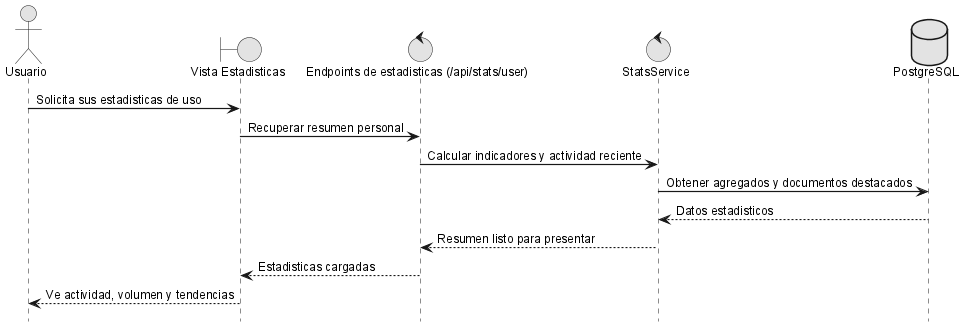
\includegraphics[width=0.9\textwidth]{diagramas/seq-user-stats.png}\caption{Secuencia de diseño — UC-0038: Estadísticas Personales}\label{fig:seq-user-stats}\end{figure}
\begin{figure}[H]\centering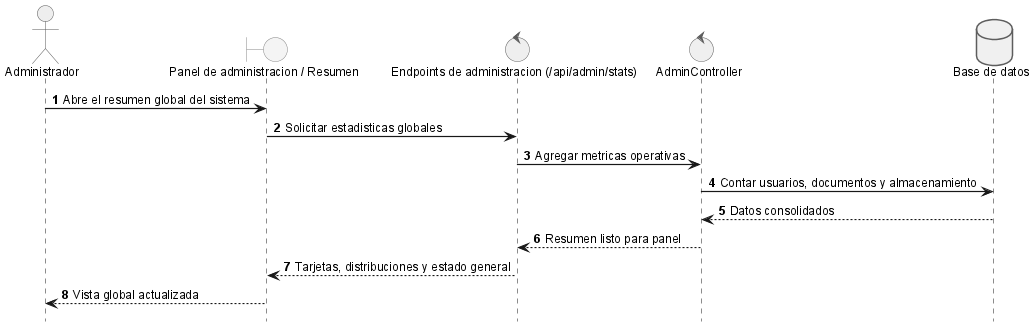
\includegraphics[width=0.9\textwidth]{diagramas/seq-global-stats.png}\caption{Secuencia de diseño — UC-0039: Estadísticas Globales}\label{fig:seq-global-stats}\end{figure}
\begin{figure}[H]\centering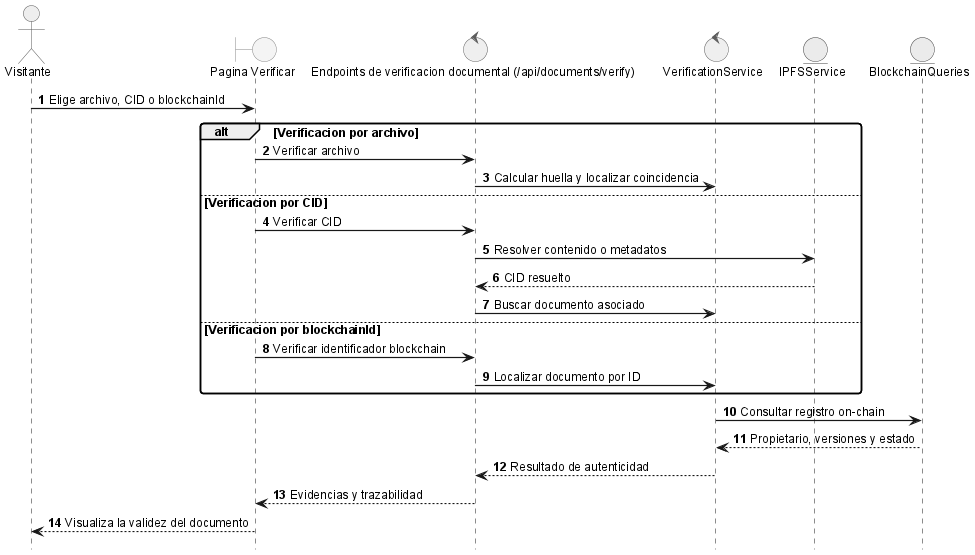
\includegraphics[width=0.9\textwidth]{diagramas/seq-verify-authenticity.png}\caption{Secuencia de diseño — UC-0040: Verificar Autenticidad}\label{fig:seq-verify-authenticity}\end{figure}
\begin{figure}[H]\centering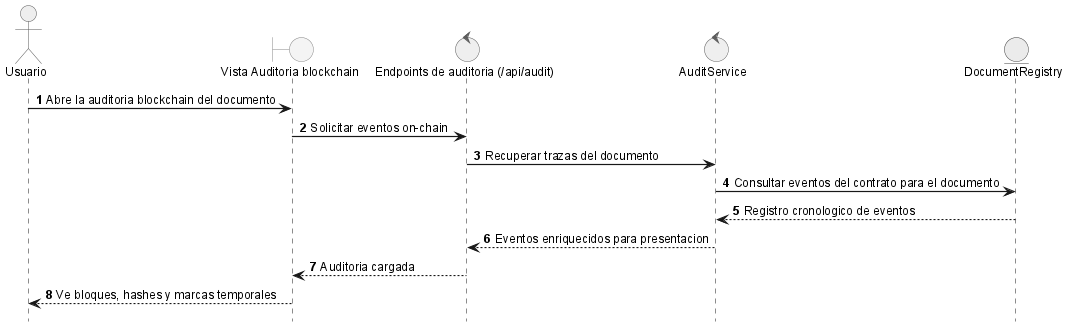
\includegraphics[width=0.9\textwidth]{diagramas/seq-blockchain-audit.png}\caption{Secuencia de diseño — UC-0041: Auditoría Blockchain}\label{fig:seq-blockchain-audit}\end{figure}
\begin{figure}[H]\centering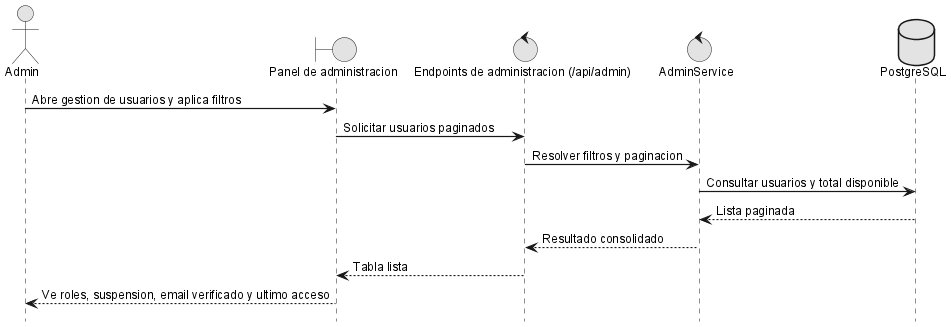
\includegraphics[width=0.9\textwidth]{diagramas/seq-list-users.png}\caption{Secuencia de diseño — UC-0042: Listar Usuarios}\label{fig:seq-list-users}\end{figure}
\begin{figure}[H]\centering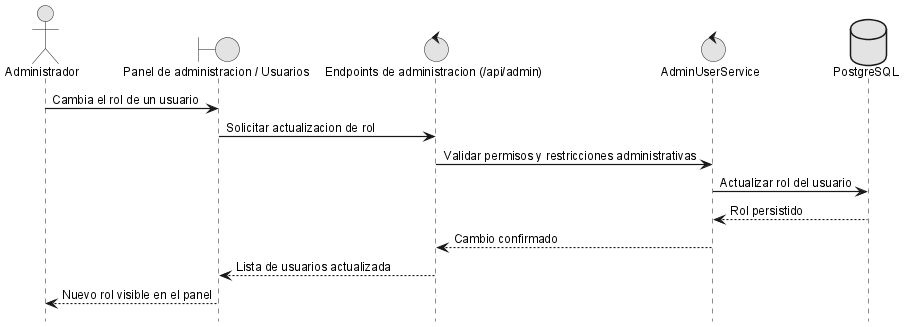
\includegraphics[width=0.9\textwidth]{diagramas/seq-manage-roles.png}\caption{Secuencia de diseño — UC-0043: Gestionar Roles}\label{fig:seq-manage-roles}\end{figure}


\section{Diseño de datos}

\subsection{Diagrama Entidad-Relación}

La base de datos PostgreSQL almacena el estado operativo del sistema: usuarios, documentos, versiones, firmas, permisos de compartición, notificaciones, eventos de auditoría y carpetas. La Figura~\ref{fig:er} presenta el diagrama entidad-relación clásico.

\begin{figure}[H]
    \centering
    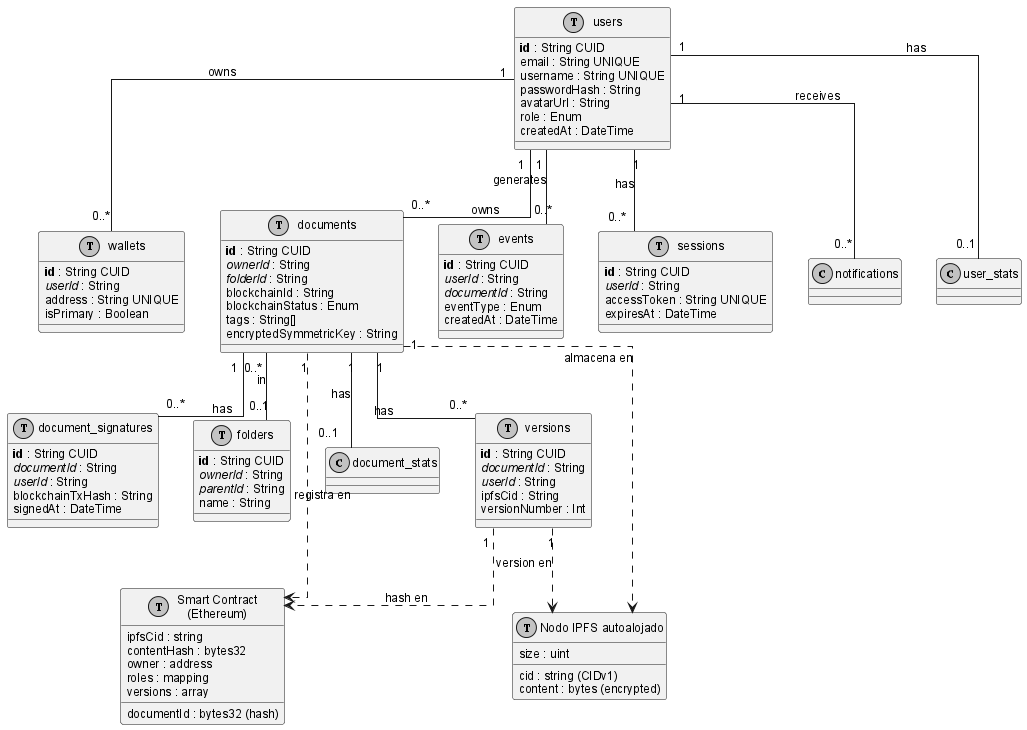
\includegraphics[width=0.92\linewidth]{diagramas/er-diagram.png}
    \caption{Diagrama Entidad-Relación de la base de datos}
    \label{fig:er}
\end{figure}

\subsection{Persistencia coordinada: PostgreSQL, IPFS y blockchain}

La Figura~\ref{fig:er-combined} integra las tres capas de persistencia en una única vista: PostgreSQL para estado relacional, IPFS para contenido binario direccionable por hash, y la blockchain para registro inmutable de operaciones. Las entidades \texttt{Document}, \texttt{Version} y \texttt{DocumentSignature} mantienen referencias cruzadas a identificadores IPFS (CID) y transacciones blockchain (txHash).

\begin{figure}[H]
    \centering
    
\includegraphics[width=\linewidth]{diagramas/er-combined.png}
    \caption{Persistencia coordinada: PostgreSQL, IPFS y blockchain}
    \label{fig:er-combined}
\end{figure}

\section{Modelo de despliegue}

La Figura~\ref{fig:deployment} presenta el modelo de despliegue del sistema. Los servicios se ejecutan en contenedores Docker independientes conectados mediante una red bridge: frontend sirviendo la SPA, backend exponiendo la API REST en el puerto 3000, PostgreSQL para persistencia, Hardhat como nodo Ethereum local de desarrollo, y Postfix como servidor SMTP. El almacenamiento documental se realiza a través de Pinata (proveedor IPFS configurado por defecto), con la posibilidad de activar un nodo Kubo autoalojado.

\begin{landscape}
\begin{figure}[H]
    \centering
    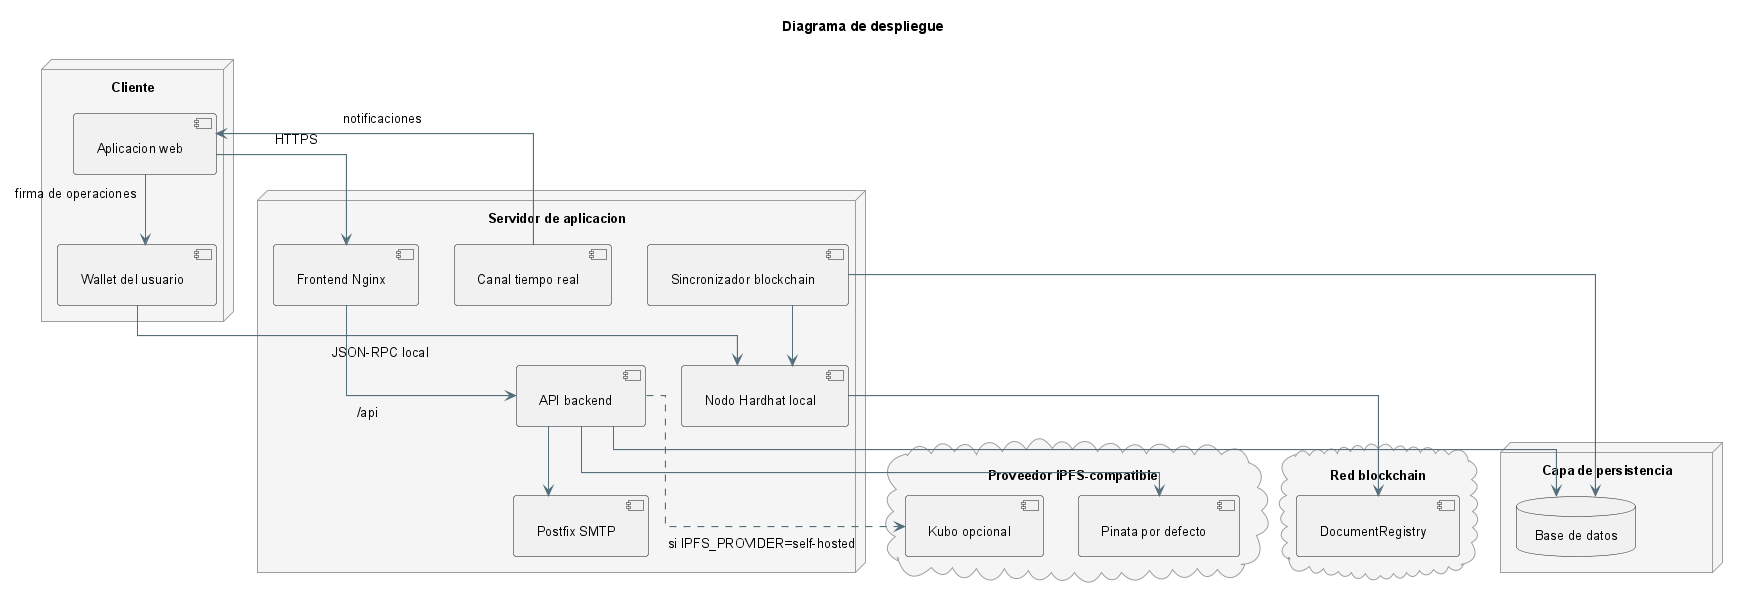
\includegraphics[width=0.95\linewidth]{diagramas/deployment.png}
    \caption{Modelo de despliegue con contenedores Docker}
    \label{fig:deployment}
\end{figure}
\end{landscape}

\section{Referencias}

\begin{enumerate}
    \item Jacobson, I., Booch, G., y Rumbaugh, J. (2000). \textit{El Proceso Unificado de Desarrollo de Software}. Addison-Wesley.
    \item Rumbaugh, J., Jacobson, I., y Booch, G. (2000). \textit{El Lenguaje Unificado de Modelado. Manual de Referencia}. Addison-Wesley.
    \item OpenZeppelin. (2024). \textit{OpenZeppelin Contracts}. \url{https://docs.openzeppelin.com/contracts}
    \item Protocol Labs. (2024). \textit{IPFS Documentation}. \url{https://docs.ipfs.io}
    \item PlantUML. (2024). \textit{PlantUML Language Reference Guide}. \url{https://plantuml.com}
    \item PostgreSQL Global Development Group. (2024). \textit{PostgreSQL 16 Documentation}. \url{https://www.postgresql.org/docs/16}
    \item Prisma. (2024). \textit{Prisma Documentation}. \url{https://www.prisma.io/docs}
\end{enumerate}

\end{document}
